% Template for the submission to:
%   Annals of Mathematical Sciences and Applications [amsa]
%
% Author: In this template, the places where you need to add information
%         (or delete line) are indicated by {???}.  Mostly the information
%         required is obvious, but some explanations are given in lines starting
% Author:
% All other lines should be ignored.  After editing, there should be
% no instances of ??? after this line.

% journal options: amsa  
\documentclass[amsa]{ipart}

\usepackage{mymacros}
%\usepackage{citesort}

%\usepackage{amsthm,amsmath}
%\usepackage[numbers,square]{natbib}
%\RequirePackage{hyperref}

% will be filled by editor:
\pubyear{2014}
\volume{0}
\issue{0}
\firstpage{1}
\lastpage{1}
%\arxiv{}

% put your definitions there:
\startlocaldefs
\endlocaldefs

\begin{document}

\begin{frontmatter}

% "Title of the Paper"
\title{Spectral analysis and computation \\
  of effective diffusivities in 
  space-time periodic incompressible flows}
%\thankstext{t1}{Title thanks}
\runtitle{Spectral analysis of space-time periodic flows}

% indicate corresponding author with \corref{}
% \author{\fnms{John} \snm{Smith}\thanksref{t2}\corref{}\ead[label=e1]{smith@foo.com}\ead[label=e2,url]{www.foo.com}}
% \thankstext{t2}{Thanks to somebody}
% \address{line 1\\ line 2\\ \printead{e1}\\ \printead{e2}}

\begin{aug} 
\author{\fnms{N. Benjamin} \snm{Murphy,}
  \thanksref{t1,t2,t3}
  \ead[label=e1]{nbmurphy@math.uci.edu}}
\address{University of California at Irvine, Department of Mathematics, 340
Rowland Hall, \\Irvine, CA 92697-3875, USA
\printead{e1}}
%\and
\author{\fnms{Elena} \snm{Cherkaev,}
  \thanksref{t2,t3}
  \ead[label=e2]{elena@math.utah.edu}}
\address{University of Utah, Department of Mathematics, 
155 South 1400 East Room 233, \\Salt Lake City, UT 84112-0090, USA
\printead{e2}}
%\and
\author{\fnms{Jack} \snm{Xin,}
  \thanksref{t1}
  \ead[label=e3]{jxin@math.uci.edu}}
\address{University of California at Irvine, Department of Mathematics, 340
Rowland Hall, \\Irvine, CA 92697-3875, USA
\printead{e3}}
%\and
\author{\fnms{Jingyi} \snm{Zhu,}
  \thanksref{t2,t3}
  \ead[label=e4]{zhu@math.utah.edu}}
\address{University of Utah, Department of Mathematics, 
155 South 1400 East Room 233, \\Salt Lake City, UT 84112-0090, USA
\printead{e4}}
\and
\author{\fnms{Kenneth M.} \snm{Golden}
  \thanksref{t2,t3}
  \ead[label=e5]{golden@math.utah.edu}}
\address{University of Utah, Department of Mathematics, 
155 South 1400 East Room 233, \\Salt Lake City, UT 84112-0090, USA
\printead{e5}}

\thankstext{t1}{NSF Grant DMS-1211179}
\thankstext{t2}{NSF Grant DMS-0940249}
\thankstext{t3}{ONR Grant N00014-12-1086}

\runauthor{Murphy et al.}

\affiliation{University of California, Irvine and University of Utah}

\end{aug}



\begin{abstract}
The enhancement in diffusive transport of passive tracer particles by
incompressible, turbulent flow fields is a challenging problem with
theoretical and practical importance in many areas of science and
engineering, ranging from the transport of mass, heat, and pollutants
in geophysical flows to sea ice dynamics and turbulent combustion. The
long time, large scale behavior of such systems is equivalent to an
enhanced diffusion process with an effective diffusivity tensor
$\Dm^*$. Two different formulations of integral representations for
$\Dm^*$ were developed for the case of \emph{time-independent} fluid
velocity fields, involving spectral measures of \emph{bounded}
self-adjoint operators acting on vector fields and scalar fields,
respectively. Here, we extend both of these approaches to the case of
\emph{space-time periodic} velocity fields, with possibly chaotic
dynamics, providing rigorous integral representations for $\Dm^*$
involving spectral measures of \emph{unbounded} self-adjoint
operators. We prove the different formulations are
equivalent. Their correspondence follows from a one-to-one isometry
between the underlying Hilbert spaces. We also develop a Fourier
method for computing $\Dm^*$, which captures the phenomenon of
residual diffusion related to Lagrangian chaos of a model flow. This
is reflected in the spectral measure by a concentration of mass near
the spectral origin.    
\end{abstract}

\begin{keyword}[class=AMS]
\kwd[Primary ]{47B15,65C60,35C15,\\76B99,76M22,76M50,76R99}
%\kwd{}
%\kwd[; secondary ]{}
\end{keyword}

\begin{keyword}
\kwd{advective diffusion}
\kwd{homogenization}
\kwd{effective diffusivity}
\kwd{spectral measure}
\kwd{integral formula}
\kwd{Fourier method}
\kwd{generalized eigenvalue computation}
\kwd{residual diffusion}
%\kwd{}
\end{keyword}

% history:
% \received{\smonth{1} \syear{0000}}

%\tableofcontents

\end{frontmatter}


\section{Introduction}\label{sec:Introduction}
The long time, large scale motion of diffusing particles or tracers
being advected by an incompressible flow field is equivalent to an
enhanced diffusion process~\cite{Taylor:PRSL:196} with an effective
diffusivity tensor $\Dm^*$. Describing the associated 
transport properties is a challenging problem with a broad range of
scientific and engineering applications, such as stellar
convection~\cite{Knobloch:1992ApJ,Press:1981:ApJ,canut98,canut98b,canut00},
turbulent
combustion~\cite{Aslanyan:BF00790149,Bilger:05:10.1016,Tabaczynski:1990:243,Williams:1985:TC:9781611971064,Peters:2000:TC:9780521660822,Xin:2009:Fronts:9780387876832},
and solute transport in porous
media~\cite{Bhattacharya:AAP:1999:951,Bhattacharya:1989:ASD,Whitaker:AIC690130308,Gupta:WRCR3940,Koch:1988:965,Lester:PRL:111.174101,Koch:JFM:7961001}.
Time-dependent flows can have fluid velocity fields with chaotic
dynamics, which gives rise to turbulence that greatly enhances the
mixing, dispersion, and large scale transport of diffusing
scalars. Here, we develop a mathematical framework that provides an
analytic representation of $\Dm^*$ for such time-dependent, chaotic
flows. This representation is given in terms of a Stieltjes integral
involving the spectral measure of an \emph{unbounded} self-adjoint
operator and the molecular diffusion constant $\varepsilon$. We demonstrate that
this approach provides an effective method for computing $\Dm^*$ for a
model, chaotic flow.  


\subsection{Advection enhanced diffusion in the climate system}
\label{sec:AD_in_the_climate}
%
In the climate
system~\cite{Csanady:1973:9789027702609,Griffies:2003:10.1007},
turbulence plays a key role in transporting mass, heat, momentum,
energy, and salt in geophysical
flows~\cite{Moffatt:RPP:621}. Turbulence enhances the dispersion of
atmospheric gases~\cite{Espinosa:MET1292} such as
ozone~\cite{Holton:JGRC2495,Pitari:JGR:1986,Plumb:JAS:1979,Plumb:JAS:1987}
and
pollutants~\cite{Bilger:10.1175,Beychok:1994:9780964458802,Samson:1988:88009978},
as well as atmosphere-ocean transfers of carbon dioxide and other
climatically important trace gas
fluxes~\cite{Zappa:2007:67613,Banerjee:10.1007}.  Longitudinal
dispersion of passive scalars in oceanic flows can be enhanced by
horizontal turbulence due to shearing of tidal currents, wind drift,
or
waves~\cite{Young:JPO:1982:515,Kullenberg:1972:TUS1529,Bowden:JFM:1965}.   
Chaotic motion of 
time-dependent fluid velocity fields cause instabilities in large
scale ocean currents, generating geostrophic
eddies~\cite{Ferrari:JPO:1501} which dominate the kinetic energy of
the ocean~\cite{Ferrari:ARFM:253}. Geostrophic
eddies greatly enhance~\cite{Ferrari:JPO:1501} the meridional mixing
of heat, carbon and other climatically important tracers, typically
more than one order of magnitude greater than the mean flow of the
ocean~\cite{Souza:OS:317}. Eddies also impact heat and salt budgets
through lateral fluxes and can extend the area of high biological
productivity offshore by both eddy chlorophyll advection and eddy
nutrient pumping~\cite{Chaigneau:JGR:C11025}. 

In sea ice dynamics,
where the ice cover couples the atmosphere to the polar
oceans \cite{Washington:1986:9780935702521}, the transport of sea 
ice can also be enhanced by eddie
fluxes and large scale coherent structures in the ocean
\cite{Watanabe:2009JPO4010,Lukovich:AG:2015}. 
In sea ice thermodynamics, the temperature field of the 
atmosphere is coupled to the temperature field of the ocean through
sea ice, which is a composite of pure ice with brine inclusions
whose volume fraction and connectedness depend strongly
on temperature.
Convective brine flow through the porous
microstructure can enhance thermal transport through the sea ice layer
\cite{Lytle:JGR-8853,Worster:PTRSA:2015,Liu:2015}.




Both numerical and observational studies of scalar transport have
suggested that tracers are advected over large scales by a fluid
velocity field that is different from the mean
flow~\cite{Pavliotis:PHD_Thesis}. This suggests that the effective
diffusivity tensor $\Dm^*$ should be spatially and possibly also
temporally inhomogeneous~\cite{Pavliotis:PHD_Thesis}. The mixing of
eddy fluxes is typically non-divergent and unable to affect the
evolution of the mean flow~\cite{Middleton:JPO:5840223}, and do not
alter the tracer moments~\cite{Griffies:JPO:1998}. In this sense, the
mixing is non-dissipative, reversible, and sometimes referred to as
stirring~\cite{Eckart:JMR:1948,Griffies:JPO:1998}. It has been noted
in various geophysical contexts~\cite{Plumb:JAS:1979,Plumb:JAS:1987}
that eddy-induced skew-diffusive tracer fluxes directed normal to
the tracer gradient~\cite{Middleton:JPO:5840223}] are generally
equivalent to \emph{antisymmetric} components in the effective
diffusivity tensor $\Dm^*$, while the \emph{symmetric} part of $\Dm^*$
represents irreversible diffusive
effects~\cite{Redi:JPO:1982:1154,Solomon:OGR:1971:233,Griffies:JPO:1998}
directed down the tracer gradient.  Motivated by these observations,
in the ensuing sections we provide analytic representations for both
the \emph{symmetric and antisymmetric} components of $\Dm^*$. 



\subsection{Mathematical characterization of effective diffusivity}
%
Due to the computational intensity of detailed climate
models~\cite{Griffies:2003:10.1007,Washington:1986:9780935702521,Neelin:2010:CCCM},
a coarse resolution is necessary in numerical simulations and
\emph{parameterization} is used to help resolve sub-grid
processes, such as turbulent 
entrainment-mixing processes in clouds~\cite{Lu:JGR:D50094},
atmospheric boundary layer turbulence~\cite{Bretherton:JOC:5655449},
atmosphere-surface exchange over the
sea~\cite{Fairall:1996:JGRC6562} and sea
ice~\cite{Sorensen:TC:2014,Andreas:2010:QJ618,Andreas:JH:2010,Vihma:2014:9923},
and eddies in the ocean~\cite{McDougall:2001:book,Gent:JPO:1995}. In
this way, only the effective or averaged behavior of these sub-grid
processes are included in the models. Here, we study the effective
behavior of advection enhanced diffusion by time-dependent fluid
velocity fields, with possibly chaotic dynamics, which gives rise to
such a parameterization, namely, the effective diffusivity tensor
$\Dm^*$ of the flow. 



In recent decades, a broad range of mathematical techniques have been
developed
%
%Advective-Diffusion:
%\cite{McLaughlin:SIAM_JAM:780,Biferale:PF:2725,Fannjiang:1994:SIAM_JAM:333,Novikov:2005:CPAM:867,Pavliotis:PHD_Thesis}
%Porous Media:
%\cite{Mauri:1991:3:743,Clark:1998:364,Hornung:1997:9780387947860}
%Books:
%\cite{Bensoussan:Book:1978,Holmes:1995:94481954}
%Stochastic DEs:
%\cite{Pavliotis:CMS:2007:507,Fannjiang:1997:1033}
%Reaction-Advection-Diffusion:
%\cite{Majda:Kramer:1999:book,Majda:1994:10.1088}
%
which reduce the analysis of enhanced diffusive transport by complex
fluid velocity fields with rapidly varying structures in both space
and time, to 
solving averaged or \emph{homogenized} equations that do not have
rapidly varying data, and involve an effective
parameter~\cite{Papanicolaou:1981:36:8,McLaughlin:SIAM_JAM:780,Bensoussan:Book:1978,Biferale:PF:2725,Fannjiang:1994:SIAM_JAM:333,Novikov:2005:CPAM:867,Fannjiang:1997:1033,Mauri:1991:3:743,Pavliotis:PHD_Thesis,Pavliotis:CMS:2007:507,Clark:1998:364,Holmes:1995:94481954,Hornung:1997:9780387947860,Majda:Kramer:1999:book,Majda:1994:10.1088,Xin:2009:Fronts:9780387876832}. Motivated
by~\cite{Papanicolaou:RF-835}, it was
shown in~\cite{McLaughlin:SIAM_JAM:780} that the homogenized behavior of
the advection-diffusion equation with a random, time-independent,
incompressible, mean-zero fluid velocity field, is given by an
inhomogeneous diffusion equation involving the symmetric part
of an effective diffusivity tensor $\Dm^*$. Moreover, a rigorous
representation of $\Dm^*$ was given in terms of an auxiliary
\emph{cell or corrector problem} involving a curl-free random
field~\cite{McLaughlin:SIAM_JAM:780}. We stress that the effective
diffusivity tensor $\Dm^*$ is not symmetric in general. However, only
its symmetric part appears in the homogenized equation for \emph{this} 
formulation of the effective transport properties of advection
enhanced diffusion~\cite{McLaughlin:SIAM_JAM:780}.    



The incompressibility condition of the time-independent fluid velocity
field was used in~\cite{Avellaneda:PRL-753,Avellaneda:CMP-339} to
transform the cell problem in~\cite{McLaughlin:SIAM_JAM:780} into the
quasi-static limit of Maxwell's
equations~\cite{Jackson-1999,Golden:CMP-473}, which describe the
transport properties of an electromagnetic wave in a composite
material~\cite{Milton:2002:TC}. The analytic continuation method for
representing transport in composites~\cite{Golden:CMP-473} provides
Stieltjes integral representations for the bulk transport coefficients
of composite media, such as electrical conductivity and permittivity,
magnetic permeability, and thermal
conductivity~\cite{Milton:2002:TC}. This method is based on the
spectral theorem~\cite{Stone:64,Reed-1980} and a resolvent formula
for, say, the electric field, involving a random self-adjoint
operator~\cite{Golden:CMP-473,Murphy:JMP:063506} or
matrix~\cite{Murphy:2015:CMS:13:4:825}. Based on the analytic
continuation method~\cite{Golden:CMP-473},
in~\cite{Avellaneda:PRL-753,Avellaneda:CMP-339} 
the cell problem for the advection diffusion equation was transformed
into a resolvent formula involving a 
\emph{bounded} self-adjoint operator, acting on the Hilbert
space of curl-free random vector
fields. This, in turn,     
led to a Stieltjes integral representation for the symmetric part of
the effective diffusivity tensor $\Dm^*$, involving the P{\'e}clet
number $\Pen$ of the flow and a \emph{spectral measure} $\bmu$ of the
operator~\cite{Avellaneda:PRL-753,Avellaneda:CMP-339}. A key feature
of the method is that parameter information in $\Pen$ is 
\emph{separated} from the complicated geometry of the time-independent
flow, which is encoded in the measure $\bmu$. This property led to
rigorous bounds~\cite{Avellaneda:CMP-339} for the diagonal components
of $\Dm^*$. Bounds for $\Dm^*$ can also be obtained using variational 
methods~\cite{Avellaneda:CMP-339,Fannjiang:1994:SIAM_JAM:333,Novikov:2005:CPAM:867,Fannjiang:1997:1033}.  



The mathematical framework developed in~\cite{McLaughlin:SIAM_JAM:780}
was also
adapted~\cite{Pavliotis:PHD_Thesis,Majda:Kramer:1999:book} 
to the case of a periodic, 
time-dependent, incompressible fluid velocity field with \emph{non-zero}
mean. The velocity field was modeled as a superposition of a
large-scale mean flow with small-scale periodically oscillating 
fluctuations. It was shown~\cite{Pavliotis:PHD_Thesis} that, depending
on the strength of the fluctuations relative to the mean flow, the
effective diffusivity tensor $\Dm^*$ can be constant or a function of
both space and time. When $\Dm^*$ is
constant, only its symmetric part 
appears in the homogenized equation as an enhancement in the
diffusivity. However, when $\Dm^*$ is a function of space and time,
its antisymmetric part also plays a key role in the homogenized
equation. In particular, the symmetric part of $\Dm^*$ appears as an
enhancement in the diffusivity, while both the symmetric and
antisymmetric parts of $\Dm^*$ contribute to an effective drift in the
homogenized equation. The effective drift due to the antisymmetric
part is purely sinusoidal, thus
divergence-free~\cite{Pavliotis:PHD_Thesis}. This is consistent with
what has been observed in geophysical flows in the climate system, as
discussed in the final paragraph of
\secref{sec:AD_in_the_climate}. 


In an alternate formulation of the effective parameter problem based  
on~\cite{Bhattacharya:AAP:1999:951}, the cell problem discussed 
in~\cite{Pavliotis:PHD_Thesis} was transformed into a resolvent formula
involving a self-adjoint operator acting on a Sobolev
space~\cite{McOwen:2003:PDE,Folland:95:PDEs} of spatially periodic scalar
fields, which is also a Hilbert space. In the case where the mean flow
and periodic fluctuations are time-independent, the
self-adjoint operator is compact~\cite{Bhattacharya:AAP:1999:951},
hence \emph{bounded}~\cite{Stakgold:BVP:2000}. This led to a
discrete Stieltjes integral representation for the
antisymmetric part of $\Dm^*$, involving the P{\'e}clet number of the
steady flow and a spectral measure of the operator.    



The incompressibility of the fluid velocity field is a central
property of the mathematical frameworks described above. However, 
these results were extended in~\cite{McLaughlin:Forest:PF:1999:880}
to weakly compressible, anelastic, stratified, time-independent,
fluid velocity fields. Homogenization of the
convection-reaction-diffusion equation with a compressible velocity
field is treated in~\cite{Papanicolaou:1995:Diff_Rand_Media}. 


\subsection{Summary of Results}
%
Here, we generalize both of the approaches described
in~\cite{Avellaneda:PRL-753,Avellaneda:CMP-339}
and~\cite{Pavliotis:PHD_Thesis} to the case of an incompressible,
periodic, \emph{time-dependent} fluid velocity field, allowing for
chaotic dynamics. In particular, for each approach, we provide Stieltjes
integral representations for both the symmetric and antisymmetric
parts of the effective diffusivity tensor $\Dm^*$, involving a
spectral measure of a self-adjoint operator. In this time-dependent
setting, the underlying operator becomes \emph{unbounded}. The
spectral theory of unbounded operators is more subtle and technically
challenging than the spectral theory of bounded operators, since the
domain of an unbounded operator and its adjoint plays a central role
in the 
spectral characterization of the operator. Neglecting such important 
mathematical details, the Stieltjes integral representation for
$\Dm^*$ given in~\cite{Avellaneda:PRL-753,Avellaneda:CMP-339} was
extended to the time-dependent setting
in~\cite{Avellaneda:PRE:3249}. Here, we provide mathematically 
rigorous formulations of Stieltjes integral representations for $\Dm^*$
in the time-dependent, unbounded operator setting. Moreover, we prove
that the two approaches 
in~\cite{Avellaneda:PRL-753,Avellaneda:CMP-339}
and~\cite{Pavliotis:PHD_Thesis} are equivalent in this setting, and
that their correspondence follows from a one-to-one isometry between
the underlying Hilbert spaces. We also establish a direct
correspondence between the effective parameter problem for $\Dm^*$ and
the analogous effective parameter problem arising in the analytic
continuation method for composite materials.  






In over 25 years since the first derivation~\cite{Avellaneda:PRL-753}
of an integral representation for the effective diffusivity tensor
$\Dm^*$, analytical calculations of the underlying spectral measure
have been obtained only for a handful of simple flows, such as
shear flow~\cite{Avellaneda:CMP-339}, and numerical computations of
the effective behavior based on this powerful representation have
apparently not been attempted. To help overcome this limitation, we
develop a Fourier method for the computation of $\Dm^*$. In
particular, we compute the effective properties for the following
space-time periodic flow in two spatial dimensions, with $\vecx=(x,y)$,
%
\begin{align}\label{eq:tdcell}
\vecu (t,\vecx)=(\cos{y},\cos{x}) + \theta\,\cos{t}\;(\sin{y},\sin{x}), 
\quad
\theta \in (0,1].
\end{align}
%
The steady part $(\cos{y}, \cos{x})$ of the flow is subject to a
time-periodic perturbation that gives rise to a transition to
Lagrangian chaos for $\theta>0$~\cite{Biferale:PF:2725,ZCX_2015}. In a
study of \emph{residual
  diffusivity}~\cite{Biferale:PF:2725,ZCX_2015} for the advection 
dominated regime, we shall compare our computations of the effective
diffusivity for the steady $\theta=0$ and dynamic $\theta=1$ settings.   



The rest of the paper is organized as follows. In
\secref{sec:Eff_Trans}, the theory of homogenization for the
advection-diffusion equation for space-time periodic flows is
reviewed. Novel Stieltjes integral representations for the effective
diffusivity tensor $\Dm^*$ are also obtained for a large class of
space-time periodic fluid velocity fields, involving a spectral
measure of an \emph{unbounded} self-adjoint operator. In
\secref{sec:Fourier_Methods}, we provide a rigorous mathematical
framework for the computation of the discrete part of the spectral
measure $\mu$ and integral representation for $\Dm^*$, providing a
rigorous lower bound for $\Dm^*$. In particular, we use
Fourier methods to transform the eigenvalue problem for the
self-adjoint operator involving the space-time periodic fluid velocity
field in equation~\eqref{eq:tdcell} into an infinite system of algebraic
equations. This framework is employed in \secref{sec:Num_Results} 
to compute the discrete component of $\Dm^*$ for the velocity field in
\eqref{eq:tdcell}, for both the time-independent $\theta=0$ and
time-dependent $\theta=1$ settings.




Our computations highlight that the
behavior of the measure 
near the spectral origin governs the behavior of the effective
diffusivity in the advection dominated regime of small molecular
diffusion. In particular, we demonstrate that for $\theta=0$ there is a
\emph{spectral gap} in the measure near a limit point at the spectral
origin, giving rise to the known vanishing asymptotic behavior of 2D
cell
flows~\cite{Fannjiang:1994:SIAM_JAM:333,Novikov:2005:CPAM:867}. However
in the time dependent setting, a strong concentration of measure mass 
near the spectral origin gives rise to the phenomenon of residual
diffusivity in the limit of vanishing molecular diffusion.




Technical background information and proofs of the key results of the
paper are differed to the appendices. The spectral theory of unbounded
self-adjoint operators in Hilbert space is reviewed in 
\appref{app:Spectral_Theory} and \appref{app:Time_Derivative}. Two
mathematical formulations of the effective parameter problem for
advection enhanced diffusion are presented in
\appref{app:Scalar_Fields} and \appref{app:Curl_Free_Fields}, leading
to novel integral representations for the symmetric and antisymmetric 
components of the effective diffusivity tensor. In
\appref{app:Isometric_Correspondence} we use powerful methods of
functional analysis to prove that the two approaches are equivalent,
which follows from a one-to-one isometry between the associated
Hilbert spaces. In \appref{app:Eig_Funct_Exp} we derive an explicit 
formula for the discrete component of the spectral measure, which is
employed in our numerical computations.





\section{Effective transport by
  advective-diffusion} \label{sec:Eff_Trans}    
%
The density $\phi$ of a cloud of passive tracer particles diffusing along
with molecular diffusivity $\varepsilon$ and being advected by an incompressible
velocity field $\vecu$ satisfies the advection-diffusion equation
%
\begin{align}\label{eq:ADE}
  \partial_t\phi(t,\vecx)
    =\vecu (t,\vecx)\bcdot\bnabla \phi(t,\vecx)+\varepsilon\Delta \phi(t,\vecx),
  \quad
  \phi(0,\vecx)=\phi_0(\vecx),  
  % \quad
%   t>0,
%   \quad
%   \vecx\in\mathbb{R}^d.
\end{align}
%
for $t>0$ and $\vecx\in\mathbb{R}^d$.
Here, the initial density $\phi_0(\vecx)$ and the fluid velocity field
$\vecu$ are assumed given, and $\vecu$ satisfies $\bnabla\bcdot\vecu=0$.
In equation~\eqref{eq:ADE}, the molecular diffusion constant $\varepsilon>0$,
$d$ is the spatial dimension of the 
system, $\partial_t$ denotes partial differentiation with respect to time
$t$, and $\Delta=\bnabla\bcdot\bnabla =\nabla^2$ is the Laplacian. Moreover, 
$\vecpsi\bcdot\vecvarphi=\vecpsi^{\,T}\overline{\vecvarphi}$,
$\vecpsi^{\,T}$ denotes transposition of the vector $\vecpsi$, and
$\overline{\vecvarphi}$ denotes component-wise complex conjugation,
with $\vecpsi\bcdot\vecpsi=|\vecpsi|^2$. Later, we will extensively use this
form of the dot product over complex fields, with built in complex
conjugation. However, we stress that 
all quantities considered in this section are \emph{real-valued}.




We consider enhanced diffusive transport by a periodic fluid velocity
field and non-dimensionalize equation~\eqref{eq:ADE} as follows. Let
$L$ and $T$ be typical length and time scales associated with the
problem of interest. Mapping to the non-dimensional variables
$t\mapsto t/T$ and $\vecx\mapsto \vecx/L$,
one finds that $\phi$ satisfies the advection-diffusion equation
in~\eqref{eq:ADE} with a non-dimensional molecular diffusivity 
$\varepsilon\mapsto T\,\varepsilon/L^{\,2}$ and velocity field $\vecu\mapsto T\,\vecu /L$. There are
several different non-dimensionalizations possible 
for the advection-diffusion equation. A detailed discussion of 
various non-dimensionalizations involving the Strouhal number, the
P{\'e}clet number, and the periodic P{\'e}clet number is given
in~\cite{McLaughlin:Forest:PF:1999:880,Majda:Kramer:1999:book}.  Here,
we focus on the long time, large scale transport characteristics of
equation~\eqref{eq:ADE} as a function of $\varepsilon$. To this end, we simply
take $T$ to be the temporal periodicity of the velocity field $\vecu$
and assume that the spatial periodicity of $\vecu$ is $L$ in all
spatial dimensions, i.e., 
%
\begin{align}\label{eq:Periodic_u}
  \vecu(t+T,\vecx)=\vecu(t,\vecx), \qquad
  \vecu(t,\vecx+L\,\vece_j)=\vecu(t,\vecx), \quad
  j=1,\ldots,d,
\end{align}
%
where $\vece_j$ is a standard basis vector in the $j$th direction. 



\subsection{Mean-zero flow}\label{sec:Mean_zero_flow}
%
In this section we will discuss the effective transport properties of
advection enhanced diffusion, as described by the advection diffusion
equation in~\eqref{eq:ADE}. We will assume in this section that the
fluid velocity field is mean-zero. The effects of a large-scale mean
flow will be discussed in \secref{sec:Mean_Flow}. 




The long time, large scale dispersion of diffusing tracer particles
being advected by an incompressible fluid velocity field is equivalent
to an enhanced diffusion process~\cite{Taylor:PRSL:196} with an
effective diffusivity tensor $\Dm^*$. In recent decades, methods of
homogenization
theory~\cite{McLaughlin:SIAM_JAM:780,Fannjiang:1994:SIAM_JAM:333,Novikov:2005:CPAM:867,Majda:Kramer:1999:book}
have been used to provide an explicit representation for
$\Dm^*$. In particular, these methods have demonstrated that the
averaged or \emph{homogenized} behavior of the advection-diffusion
equation in~\eqref{eq:ADE}, with space-time periodic velocity field
$\vecu$, is determined by a diffusion equation
involving an averaged scalar density $\bar{\phi}$ and an
%(constant)
effective diffusivity tensor
$\Dm^*$~\cite{Majda:Kramer:1999:book}       
%
\begin{align}\label{eq:phi_bar}
 \partial_t\bar{\phi}(t,\vecx)=\bnabla\bcdot[\Dm^*\bnabla \bar{\phi}(t,\vecx)], \quad
  \bar{\phi}(0,\vecx)=\phi_0(\vecx).
\end{align}




Equation~\eqref{eq:phi_bar}
follows from the assumption that the
initial tracer density $\phi_0$ varies slowly relative to the variations
of the fluid velocity field 
$\vecu$~\cite{McLaughlin:SIAM_JAM:780,Fannjiang:1997:1033,Majda:Kramer:1999:book}.
This information is incorporated into equation~\eqref{eq:ADE} by
introducing a small dimensionless parameter $\delta\ll1$ and
writing~\cite{McLaughlin:SIAM_JAM:780,Fannjiang:1997:1033,Majda:Kramer:1999:book}      
%
\begin{align}
  \phi(0,\vecx)=\phi_0(\delta\vecx). 
\end{align}
%
Anticipating that $\phi$ will have diffusive dynamics as $t\to\infty$, space and 
time are rescaled according to the standard diffusive relation
%
\begin{align}\label{eq:Fast_Vars}
  \vecxi=\vecx/\delta, \quad
  \tau= t/\delta^\gamma,
  \qquad
  \gamma=2.
\end{align}
%
The rescaled form of equation~\eqref{eq:ADE} is given
by~\cite{Majda:Kramer:1999:book}  
%
\begin{align}\label{eq:ADE_delta}
  \partial_t\phi^\delta(t,\vecx)=\delta^{-1}\vecu(t/\delta^2,\vecx/\delta)\bcdot\bnabla\phi^\delta(t,\vecx)
              +\varepsilon\Delta\phi^\delta(t,\vecx),
              \quad
             \phi^\delta(0,\vecx)=\phi_0(\vecx), 
\end{align}
%
where we have denoted $\phi^\delta(t,\vecx)=\phi(t/\delta^2,\vecx/\delta)$.
The convergence of $\phi^\delta$  to $\bar{\phi}$
 can be rigorously established in the following
sense~\cite{Majda:Kramer:1999:book}   
%
\begin{align}\label{eq:Homogenization_Theorem}
  \lim_{\delta\to0}\;\sup_{0\leq t\leq t_0}\,\sup_{\vecx\in\mathbb{R}^d}
  |\phi^\delta(t,\vecx)-\bar{\phi}(t,\vecx)| =0,
\end{align}
%
for every finite $t_0>0$, provided that $\phi_0$ and $\vecu$ obey some
mild smoothness and boundedness conditions, and that $\vecu$ is
\emph{mean-zero}.  We will discuss the consequences of a fluid
velocity field $\vecu$ with a large scale mean flow in
\secref{sec:Mean_Flow}. 




An explicit representation of the
effective diffusivity tensor $\Dm^*$ is given in terms of the (unique)
mean zero, space-time periodic solution $\chi_j$ of the following
\emph{cell problem}~\cite{Biferale:PF:2725,Majda:Kramer:1999:book}, 
%
\begin{align}\label{eq:Periodic_Cell_Prob}
  \partial_\tau\chi_j(\tau,\vecxi)
  -\varepsilon\Delta_\xi\chi_j(\tau,\vecxi)
  -\vecu(\tau,\vecxi) \bcdot\bnabla_\xi \chi_j(\tau,\vecxi)
  =u_j(\tau,\vecxi),
\end{align}
%
where the subscript $\xi$ in $\Delta_\xi$ and $\bnabla_\xi$
indicates that differentiation is with respect to the fast variable
$\vecxi$ defined in equation~\eqref{eq:Fast_Vars}. The components
$\Dm^*_{jk}$, $j,k=1,\ldots,d$, of the matrix $\Dm^*$ are given 
by~\cite{McLaughlin:SIAM_JAM:780,Fannjiang:1994:SIAM_JAM:333,Novikov:2005:CPAM:867,Majda:Kramer:1999:book}          
%
\begin{align}\label{eq:Djk}
  \Dm^*_{jk}=\varepsilon\delta_{jk}+\langle u_j\chi_k\rangle,
\end{align}
%
where $\delta_{jk}$ is the Kronecker delta and $u_j$ is the $j$th component
of the vector $\vecu$. The averaging $\langle\cdot\rangle$ in~\eqref{eq:Djk} is with
respect to the fast variables defined in
equation~\eqref{eq:Fast_Vars}. The averaging is over the bounded
sets $\Tc\subset\mathbb{R}$ and $\Vc\subset\mathbb{R}^d$, with $\tau\in\Tc$ and
$\vecxi\in\Vc$, which define the space-time period cell ($(d+1)$--torus)
$\Tc\times\Vc$. For example, in \secref{sec:Num_Results} we compute $\Dm^*$
for the fluid velocity field $\vecu$ in~\eqref{eq:tdcell} with
temporal periodicity $\Tc=[0,2\pi]$ and spatial periodicity
$\Vc=[0,2\pi]^d$, with $d=2$. In the case of a 
time-dependent fluid velocity field, $\langle\cdot\rangle$ 
denotes space-time averaging over $\Tc\times\Vc$. In the special case of a
time-independent fluid velocity field, the function $\chi_j$ is
time-independent and satisfies equation~\eqref{eq:Periodic_Cell_Prob}
with $\partial_\tau\chi_j\equiv0$, and $\langle\cdot\rangle$ in~\eqref{eq:Djk} denotes spatial averaging over
$\Vc$~\cite{Fannjiang:1994:SIAM_JAM:333,Novikov:2005:CPAM:867,Majda:Kramer:1999:book}.






\subsection{The effect of large scale mean flow}\label{sec:Mean_Flow}
%
The periodic homogenization theorem summarized by
equations~\eqref{eq:Periodic_u}--\eqref{eq:Djk}
%
% as well as its many
% variations~\cite{Bensoussan:Book:1978,Papanicolaou:1981:36:8,Bhattacharya:1985:AnnProb:13:2:385,Bhattacharya:1989:ASD,McLaughlin:SIAM_JAM:780,Avellaneda:CMP-339,Pavliotis:PHD_Thesis,Pavliotis:IMAJAM:951,Pavliotis:CMS:2007:507,McLaughlin:Forest:PF:1999:880,Majda:Kramer:1999:book},
%
depends on the detailed nature of the fluid velocity field
$\vecu$. It also depends on the temporal scaling
used~\cite{Bhattacharya:1989:ASD,Pavliotis:PHD_Thesis,Majda:Kramer:1999:book},
i.e., what value of $\gamma$ is used in
equation~\eqref{eq:Fast_Vars}. However, the mathematical structure of
the cell problem in~\eqref{eq:Periodic_Cell_Prob} and the functional
form of $\Dm^*$ shown in equation~\eqref{eq:Djk} remain unchanged for 
the space-time periodic setting.  
In order to illustrate the rich behaviors that can arise in the
effective diffusivity tensor $\Dm^*$ for more general velocity fields
and alternate temporal scalings, we now discuss some key
variations of the theory described above.







In general, the effective diffusivity tensor $\Dm^*$ has a symmetric
$\Sm^*$ and antisymmetric $\Am^*$ part defined by 
%
\begin{align}\label{eq:Symm_Anti-Symm}
  \Dm^*=\Sm^*+\Am^*,\qquad
  \Sm^*=\frac{1}{2}\left(\Dm^*+[\Dm^*]^{\,T}\right), \quad
  \Am^*=\frac{1}{2}\left(\Dm^*-[\Dm^*]^{\,T}\right),
\end{align}
%
where $[\Dm^*]^{\,T}$ denotes transposition of the matrix
$\Dm^*$. Denote by $\Sm^*_{jk}$ and $\Am^*_{jk}$, $j,k=1,\ldots,d$, the
components of $\Sm^*$ and $\Am^*$ in~\eqref{eq:Symm_Anti-Symm}.
When the fluid velocity field is mean-zero and divergence-free, as
discussed above, then 
equation~\eqref{eq:Homogenization_Theorem} holds and the effective
diffusivity tensor $\Dm^*$ defined in~\eqref{eq:Djk} is
constant~\cite{Majda:Kramer:1999:book}. Consequently, only the symmetric part of $\Dm^*$ plays a role in the effective transport
equation shown in~\eqref{eq:phi_bar}~\cite{Pavliotis:PHD_Thesis}.




Now consider the  more general, divergence-free fluid velocity field
%$\vecu(t,\vecx,\tau,\vecxi)=\delta\vecu_0(\delta^2t,\delta\vecx)+\vecu_1(t,\vecx)$
%
\begin{align}\label{eq:Velocity_field_uo_u1}
  \vecu(t,\vecx)=\delta\vecu_0(\delta^2 t,\delta\vecx)+\vecu_1(t,\vecx),
  % \vecu(t,\vecx)=\delta^\alpha\vecu_0(\delta^\gamma t,\delta\vecx)+\vecu_1(t,\vecx),
%   \qquad
%   \alpha=1, \quad
%   \gamma=2,
\end{align}
%
which is the superposition of a \emph{weak}, large-scale mean flow
$\delta\vecu_0(\delta^2t,\delta\vecx)$ that varies on large spatial and slow time
scales, with a mean-zero periodic flow $\vecu_1(t,\vecx)$ that rapidly
fluctuates in space and time~\cite{Majda:Kramer:1999:book}.
If $\vecu_0(t,\vecx)$ is smooth and bounded, the homogenization
theorem for purely periodic velocity fields discussed above can be
rigorously extended to the present setting and the effective transport
equation in~\eqref{eq:phi_bar} is replaced
by~\cite{Majda:Kramer:1999:book}   
%
\begin{align}\label{eq:phi_bar_uo}
  \partial_t\bar{\phi}(t,\vecx)=\vecu_0(t,\vecx)\bcdot\bnabla\bar{\phi}(t,\vecx)
                   +\bnabla\bcdot[\Dm^*\bnabla\bar{\phi}(t,\vecx)],
  \quad 
  \bar{\phi}(0,\vecx)=\phi_0(\vecx),
\end{align}
%
which includes an advective enhancement in transport by the
large-scale mean flow $\vecu_0$~\cite{Majda:Kramer:1999:book}. In this
case, the effective diffusivity tensor $\Dm^*$ is completely
independent of the mean flow $\vecu_0$, and is determined by the same
formula in equation~\eqref{eq:Djk} and the same cell problem
in~\eqref{eq:Periodic_Cell_Prob} with
$\vecu$ replaced by the \emph{mean-zero} velocity field
$\vecu_1$~\cite{Majda:Kramer:1999:book}. Consequently, $\Dm^*$  
is again constant and only the symmetric part of $\Dm^*$ plays
a role in the effective transport equation shown
in~\eqref{eq:phi_bar_uo}.



In~\cite{Pavliotis:PHD_Thesis}, $\Dm^*$ was studied for the 
divergence-free fluid velocity field,
%
\begin{align}
  \vecu(t,\vecx)=\vecu_0(t,\vecx)+\delta^\alpha\vecu_1(t/\delta^\gamma,\vecx/\delta),
\end{align}
%
for a broad range of scaling parameters $\gamma$ and $\alpha$. The parameter $\gamma$
controls the separation of time scales while $\alpha$ determines the
strength of the small scale periodic fluctuations $\vecu_1$ relative
to the mean flow $\vecu_0$. There are three distinct behaviors that
arise as the values of $\alpha$ and $\gamma$ vary, and the function $\chi_j$
in the analogue of the cell problem in~\eqref{eq:Periodic_Cell_Prob}
can be time-dependent or  time-independent
$(\partial_\tau\chi_j\equiv0)$~\cite{Pavliotis:PHD_Thesis}. However, 
regardless of the values of $\alpha$ and $\gamma$ studied
in~\cite{Pavliotis:PHD_Thesis}, when the mean flow is is weak compared
to the fluctuations, to leading order, $\Dm^*$ is constant and
independent of the mean flow, which only determines the transport
velocity on large length and long time scales, similar to
equation~\eqref{eq:phi_bar_uo}. Consequently, only the symmetric part
of $\Dm^*$ plays a role in the effective transport equation, which is
similar to the effective transport equation
in~\eqref{eq:phi_bar_uo}~\cite{Pavliotis:PHD_Thesis}.   However we
stress that in all three cases, the components $\Dm^*_{jk}$ of the
effective diffusivity tensor are given by a formula analogous to
equation~\eqref{eq:Djk} and the structure of the cell problem is
analogous to equation~\eqref{eq:Periodic_Cell_Prob}, where the
velocity field component arising the right side of the cell
problem is \emph{mean-zero}.  



The effective diffusivity tensor $\Dm^*$ being constant is \emph{not}
consistent with measurements and numerical simulations of passive
tracer transport in 
the ocean and the atmosphere, as we discussed in the final paragraph of  
\secref{sec:AD_in_the_climate}. However, when the fluid velocity field
is active on both the slow and fast time scales,
$\vecu=\vecu(t,\vecx,t/\delta,\vecx/\delta)$, and the mean flow 
$\vecu_0(t,\vecx)=\langle\vecu(t,\vecx,t/\delta,\vecx/\delta)\rangle$ is
equal in strength or stronger than the 
periodic fluctuations, then the effective transport equation is
analogous to equation~\eqref{eq:phi_bar_uo} and $\Dm^*$
\emph{is a function of both space and
  time}~\cite{Pavliotis:PHD_Thesis}, $\Dm^*=\Dm^*(t,\vecx)$.  Consequently, in the effective
transport equation, the \emph{antisymmetric} part of $\Dm^*(t,\vecx)$
contributes to a 
purely rotational (divergence-free) enhancement in advective
transport, while the symmetric part of $\Dm^*(t,\vecx)$ contributes to an
enhancement in advective and diffusive
transport~\cite{Pavliotis:PHD_Thesis}. This is consistent with
observations and numerical simulations of geophysical flows in
the climate system.



We stress that, in this formulation~\cite{Pavliotis:PHD_Thesis},
the components $\Dm^*_{jk}(t,\vecx)$, $j,k=1,\ldots,d$, of the effective
diffusivity tensor are
given by a formula that is analogous to
equation~\eqref{eq:Djk}. However, the function $u_j$ appearing
in~\eqref{eq:Djk} is replaced by the $j$th component of
$\vecu(t,\vecx,t/\delta,\vecx/\delta)-\vecu_0(t,\vecx)$ which is
\emph{mean-zero}. Moreover, in this
formulation~\cite{Pavliotis:PHD_Thesis}, the cell problem is given by
a formula that is analogous to equation~\eqref{eq:Periodic_Cell_Prob}.
However the function $u_j$ appearing on the right side
of~\eqref{eq:Periodic_Cell_Prob} is again replaced by the $j$th
component of $\vecu-\vecu_0$ which is \emph{mean-zero}. We show in
\appref{app:Hilbert_Resolvent_Integral_Reps} that the essential
conditions necessary for Stieltjes integral representations for  the
symmetric $\Sm^*$ and antisymmetric $\Am^*$ parts of $\Dm^*$ 
are: 1) the fluid velocity field $\vecu$ is \emph{divergence free} and
2) the function $u_j$ appearing in~\eqref{eq:Djk} and on the right
side of equation~\eqref{eq:Periodic_Cell_Prob} is
\emph{mean-zero}. Consequently, the Stieltjes integral representations
for $\Sm^*$ and $\Am^*$ discussed in the following section hold for all of
the fluid velocity fields discussed in this section. 












\subsection{Integral representations for the effective diffusivity}
%
In \appref{app:Scalar_Fields} we provide a mathematically rigorous
framework that leads to Stieltjes integral representations for the
effective diffusivity tensor $\Dm^*$ for space-time periodic
flows. This formulation is based on the 
spectral theorem for \emph{unbounded} self-adjoint operators in
Hilbert space. In Appendices~\numappref{app:Spectral_Theory} 
and~\numappref{app:Time_Derivative}, we review the spectral theory 
of 
unbounded operators. In  \appref{app:Hilbert_Resolvent_Integral_Reps}
we give two natural Hilbert space formulations of the effective
parameter problem for $\Dm^*$ which lead to its integral
representations. In \appref{app:Isometric_Correspondence} we prove
that the two different formulations are equivalent.   





In this section we summarize the results of
\appref{app:Scalar_Fields}, which provide 
Stieltjes integral representations for both the symmetric $\Sm^*$ and
antisymmetric $\Am^*$ parts of $\Dm^*$. Since the analysis in this 
section involves only the fast variables $(\tau,\vecxi)$ defined
in equation~\eqref{eq:Fast_Vars}, for notational simplicity,
we will drop the subscripts $\xi$ shown in
equation~\eqref{eq:Periodic_Cell_Prob} and use $\partial_t$ to denote $\partial_\tau$.




In \appref{app:Scalar_Fields} we inserted the expression for $u_j$ on
the right side of~\eqref{eq:Periodic_Cell_Prob}
into equation~\eqref{eq:Djk}, which leads to the following functional
representations for the components $\Sm^*_{jk}$ and $\Am^*_{jk}$,
$j,k=1,\ldots,d$, of $\Sm^*$ and $\Am^*$~\cite{Pavliotis:PHD_Thesis}      
%
\begin{align}\label{eq:Eff_Diffusivity_Sobolev}
  \Sm^*_{jk}=\varepsilon(\delta_{jk}+\langle\chi_j,\chi_k\rangle_{1,2}),
  \quad
  \Am^*_{jk}=\langle A\chi_j,\chi_k\rangle_{1,2}\,,
  \quad
  A=(-\Delta)^{-1}(\partial_t-\vecu \bcdot\bnabla).
\end{align}
%
Here, $\langle f,h\rangle_{1,2}=\langle\bnabla f\bcdot\bnabla h\rangle$ is a Sobolev-type
\emph{sesquilinear} inner-product~\cite{McOwen:2003:PDE} and the
operator $(-\Delta)^{-1}$ is based on convolution with respect to the
Green's function for the Laplacian $\Delta$~\cite{Stakgold:BVP:2000}. 
Since the function $\chi_j$ is
\emph{real-valued} we have $\langle\chi_j,\chi_k\rangle_{1,2}=\langle\chi_k,\chi_j\rangle_{1,2}$, which implies that
$\Sm^*$ is a symmetric matrix. The function $A\chi_j$ is also
real-valued. We establish in \appref{app:Scalar_Fields} that the
operator $A$ is skew-symmetric on a suitable Hilbert space, which
implies that
$\Am^*_{kj}=\langle A\chi_k,\chi_j\rangle_{1,2}=-\langle\chi_k,A\chi_j\rangle_{1,2}=-\langle A\chi_j,\chi_k\rangle_{1,2}=-\Am^*_{jk}$
which, in turn, implies that $\Am^*$ is an antisymmetric matrix, hence
$\Am^*_{kk}=\langle A\chi_k,\chi_k\rangle_{1,2}=0$.  



Applying the linear operator $(-\Delta)^{-1}$ to both sides of the cell
problem in equation~\eqref{eq:Periodic_Cell_Prob} yields the following
resolvent formula for $\chi_j$ 
%
\begin{align}\label{eq:Resolvent_Rep_Scalar}
  \chi_j=(\varepsilon+A)^{-1}g_j, \qquad 
  %A=\Delta^{-1}(\vecu \bcdot\bnabla -\partial_t), \quad
  g_j=(-\Delta)^{-1}u_j.
\end{align}
%
From equations~\eqref{eq:Eff_Diffusivity_Sobolev}
and~\eqref{eq:Resolvent_Rep_Scalar} we have the following functional
formulas for $\Sm^*_{jk}$ and $\Am^*_{jk}$ involving the
skew-symmetric operator $A$
%
\begin{align}\label{eq:Eff_Diff_Resolvent_Sobolev}
 \Sm^*_{jk}&=\varepsilon\left(\delta_{jk}
  +\langle(\varepsilon+A)^{-1}g_j,(\varepsilon+A)^{-1}g_k\rangle_{1,2}\right), 
  \\
 \Am^*_{jk}&=\langle A(\varepsilon+A)^{-1}g_j,(\varepsilon+A)^{-1}g_k\rangle_{1,2}.
 \notag
\end{align}
%
Since $A$ is a skew-symmetric operator, it can be written as $A=\imath M$
where $M$ is a symmetric operator~\cite{Stone:64}. We demonstrate in
\appref{app:Scalar_Fields} that $M$ is \emph{self-adjoint} on an
appropriate, dense subset of a Hilbert space.



The spectral theorem for self-adjoint operators states that there is a
one-to-one correspondence between the self-adjoint operator $M$ and a
family of self-adjoint projection operators $\{Q(\lambda)\}_{\lambda\in\Sigma}$ --- the
resolution of the identity --- that satisfies
$\lim_{\lambda\to\,\inf{\Sigma}}Q(\lambda)=0$ and
$\lim_{\lambda\to\,\sup{\Sigma}}Q(\lambda)=I$~\cite{Stone:64}. Here, $\Sigma$ is the
\emph{spectrum} of the operator $M$, while $0$ and $I$ denote the null
and identity operators. Define the \emph{complex valued} function
$\mu_{jk}(\lambda)=\langle Q(\lambda)g_j,g_k\rangle_{1,2}$, $j,k=1,\ldots,d$, where  $g_j=(-\Delta)^{-1}u_j$ is defined
in~\eqref{eq:Resolvent_Rep_Scalar}. The real, $\Real\mu_{jk}(\lambda)$, and
imaginary, $\Imag\mu_{jk}(\lambda)$, parts of the function $\mu_{jk}(\lambda)$ are
strictly increasing and of bounded variation, and therefore have
Stieltjes measures $\Real\mu_{jk}$ and $\Imag\mu_{jk}$ associated with
them~\cite{Stone:64}. The function $\mu_{kk}(\lambda)$ is positive hence
$\mu_{kk}$ is a positive measure, while $\Real\mu_{jk}$ and $\Imag\mu_{jk}$,
$j\neq k$, are signed measures. Given certain regularity conditions on the
components $u_j$ of the fluid velocity field $\vecu$, the functional
formulas for $\Sm^*_{jk}$ and $\Am^*_{jk}$
in~\eqref{eq:Eff_Diff_Resolvent_Sobolev} have the following
Radon--Stieltjes integral representations, for all $0<\varepsilon<\infty$ (see
\appref{app:Scalar_Fields} for details) 
%
\begin{align}\label{eq:Integral_Rep_kappa*}
  \Sm^*_{jk}=\varepsilon\left(\delta_{jk}+\int_{-\infty}^\infty\frac{\d\Real\,\mu_{jk}(\lambda)}{\varepsilon^2+\lambda^2}\right),
  \qquad
  \Am^*_{jk}=-\int_{-\infty}^\infty\frac{\lambda\,\d\Imag\,\mu_{jk}(\lambda)}{\varepsilon^2+\lambda^2}\,.         
\end{align}
%



The integral formulas in~\eqref{eq:Integral_Rep_kappa*} involve
a spectral measure $\mu_{jk}$, $j,k=1,\ldots,d$, which has discrete and
continuous components~\cite{Reed-1980,Stone:64}. The self-adjoint
operator $M=-\imath A$ has \emph{real} eigenvalues $\lambda_l$ and orthonormal
eigenfunctions $\varphi_l$, $l=0,1,2,\ldots$, satisfying $M\varphi_l=\lambda_l\varphi_l$ and
$\langle\varphi_i,\varphi_l\rangle_{1,2}=\delta_{il}$. In \appref{eq:Gen_Methods} we employ an 
abstract mathematical framework to show the discrete parts
$\tilde{\Sm}^*_{jk}$ and $\tilde{\Am}^*_{jk}$ of the integral representations
in~\eqref{eq:Integral_Rep_kappa*} have the following series
representations involving the $\lambda_l$ and $\varphi_l$ (see
equation~\eqref{eq:Stieltjes-Radon_Rep})
%
\begin{align}\label{eq:disc_Integral_Rep_kappa*}
  \tilde{\Sm}^*_{jk}=\varepsilon\left(\delta_{jk}+
    \sum_{l=0}^\infty\frac{\Real m_{jk}(l)}{\varepsilon^2+\lambda_l^2}
  \right),
  \qquad
  \tilde{\Am}^*_{jk}
  =-\sum_{l=0}^\infty\frac{\lambda_l\;\Imag m_{jk}(l)}{\varepsilon^2+\lambda_l^2}\,.
  %\quad m^l_{jk}=\langle u_j,\varphi_l\rangle\,\overline{\langle u_k,\varphi_l\rangle}
  %\notag
\end{align}
%
Here, the \emph{spectral weights} $m_{jk}(l)$ are given by (see
equation~\eqref{eq:H1_L2}) 
% $m_{jk}(l)=\langle u_j,\varphi_l\rangle\,\overline{\langle u_k,\varphi_l\rangle}$ and the sesquilinear
% inner-product $\langle\cdot,\cdot\rangle$ is given by
% $\langle u_j,\varphi_l\rangle=\langle u_j\;\overline{\varphi_l}\rangle$.
%
\begin{align}\label{eq:Spec_Weights}
  m_{jk}(l)=\langle g_j,\varphi_l\rangle_{1,2}\;\overline{\langle g_k,\varphi_l\rangle}_{1,2},
  \qquad
  \langle g_j,\varphi_l\rangle_{1,2}=\langle u_j,\varphi_l\rangle=\langle u_j\;\overline{\varphi_l}\rangle.
\end{align}
%
In the setting of a time-independent fluid velocity field
$\vecu=\vecu(\vecx)$, the self-adjoint operator $M$ is given by
$M=-\imath(-\Delta)^{-1}[\vecu\bcdot\bnabla]$. If $\vecu$ is smooth and
uniformly bounded on $\Vc$, then $M$ is a compact
operator~\cite{Bhattacharya:AAP:1999:951} and therefore has only
discrete spectrum with a limit point at
$\lambda=0$~\cite{Stakgold:BVP:2000,Reed-1980}. Consequently, the spectral
measure $\mu_{jk}$ is purely discrete, hence
$\Dm^*_{jk}\equiv\tilde{\Dm}^*_{jk}$.
Since 
$\mu_{kk}$ is a \emph{positive measure}, the discrete integral
representation of $\tilde{\Sm}^*_{kk}$
in~\eqref{eq:disc_Integral_Rep_kappa*} provides a rigorous lower bound
for the integral representation of $\Sm^*_{kk}$ in
equation~\eqref{eq:Integral_Rep_kappa*}, 
%
\begin{align}\label{eq:LB:Skk}
  \Sm^*_{kk}\geq\tilde{\Sm}^*_{kk}.  
\end{align}
%











It is worth noting that using
$\overline{\langle g_k,\varphi_l\rangle}_{1,2}=\langle\varphi_l,g_k\rangle_{1,2}$ and Dirac 
notation $\langle\bnabla g_j\bcdot\bnabla\varphi_l\rangle=\langle\bnabla g_j|\bnabla\varphi_l\rangle$, we
may formally write the spectral weights in
equation~\eqref{eq:Spec_Weights} as
%
\begin{align}\label{eq:mjk_Dirac}
  m_{jk}(l)%=\langle g_j,\varphi_l\rangle_{1,2}\;\overline{\langle g_k,\varphi_l\rangle}_{1,2}
        &=\langle\bnabla g_j|\bnabla\varphi_l\rangle\,\langle\bnabla\varphi_l|\bnabla g_k\rangle
        \\\notag
        &=\langle\bnabla
        g_j|\,\bnabla\;[\,|\varphi_l\rangle\,\langle\bnabla\varphi_l|\,\bnabla\,]\;|g_k\rangle
        \\\notag
        &=\langle\bnabla g_j|\bnabla Q_l\,g_k\rangle,
        \notag 
\end{align}
%
where the operator $Q_l$ is given by
$Q_l=|\varphi_l\rangle\,\langle\bnabla\varphi_l|\,\bnabla\,$. In a similar way, we may use
$\overline{\langle g_k,\varphi_l\rangle}_{1,2}=\langle\varphi_l,g_k\rangle_{1,2}$ to instead
write the spectral weights in equation~\eqref{eq:mjk_Dirac} as
$m_{jk}(l)=\langle\bnabla Q_l\,g_j|\bnabla g_k\rangle$, hence $Q_l$ is a symmetric
operator with respect to the inner-product $\langle\cdot,\cdot\rangle_{1,2}$. Since
$\langle\bnabla\varphi_i|\bnabla\varphi_l\rangle=\delta_{il}$ it is clear that the $Q_l$ are
mutually orthogonal projection operators $Q_iQ_l=\delta_{il}Q_i$. With this
notation, we may formally identify the self-adjoint projection
operator $Q(\lambda)$ and the spectral measure
$\d\mu_{jk}(\lambda)=\d\langle\bnabla Q(\lambda)g_j|\bnabla g_k\rangle$ as 
%
\begin{align}
  Q(\lambda)=\sum_{l\,:\;\lambda_l\leq\lambda}\theta(\lambda-\lambda_l)\;Q_l,
  \quad
  \d\mu_{jk}(\lambda)=\sum_{l\,:\;\lambda_l\leq\lambda}\delta_{\lambda_l}(\d\lambda)\langle\bnabla Q_l\,g_j|\bnabla g_k\rangle,
\end{align}
%
where $\theta(\lambda)$ is the Heaviside function and $\delta_{\lambda_l}(\d\lambda)$ is the Dirac
$\delta$-measure concentrated at $\lambda_l$. This formula is \emph{precisely} true
for the matrix setting, where the $Q_l$ are given by mutually
orthogonal projection matrices, $\bnabla$ is given by a finite
difference matrix, and $g_j$ is a Euclidean
vector~\cite{Murphy_Advective_Diffusion_Steady}.  


 

A key feature of equations~\eqref{eq:Integral_Rep_kappa*}
and~\eqref{eq:disc_Integral_Rep_kappa*} is that 
parameter information in $\varepsilon$ is \emph{separated} from the complicated
geometry and dynamics of the time-dependent flow, which are encoded
in the spectral measure $\mu_{jk}$. This important property of the integrals
in~\eqref{eq:Integral_Rep_kappa*} follows from the
non-dimensionalization of the advection-diffusion equation discussed
in the paragraph leading 
to equation~\eqref{eq:Periodic_u}, yielding a spectral measure $\mu_{jk}$ that
is \emph{independent} of the molecular diffusivity $\varepsilon$. An alternate
formulation of the effective parameter problem for advection-diffusion
by time-dependent flows was discussed in~\cite{Avellaneda:PRE:3249},
which used a different 
non-dimensionalization, yielding a Stieltjes integral representation
for $\Sm^*_{kk}$ involving the P{\'e}clet number $\Pen$ of the flow and a
spectral measure that depends on the Strouhal number. However, as pointed
out in~\cite{Bonn:McLaughlin:JFM:2001:345}, the Strouhal number
dependence of the measure led to an implicit
dependence of the spectral measure on $\Pen$. This restricts the
utility of the integral representations, such as rigorous
bounds~\cite{Baker:1996:Book:Pade,Golden:CMP-473} which depend
explicitly on $\Pen$ but also implicitly on $\Pen$ through the
moments of the measure. Our formulation has no such restrictions. 




  
\section{Fourier methods}
\label{sec:Fourier_Methods} 
%
In equation~\eqref{eq:disc_Integral_Rep_kappa*} we provided series
representations for the discrete parts of the integral representations
for $\Sm^*_{jk}$ and $\Am^*_{jk}$ shown
in~\eqref{eq:Integral_Rep_kappa*}. These series involve the  
\emph{real} 
eigenvalues $\lambda_l$, $l=0,1,2,\ldots$, and orthonormal eigenfunctions $\varphi_l$ 
of the self-adjoint operator $M=-\imath A$, where $M\varphi_l=\lambda_l\varphi_l$,
$\langle\varphi_i,\varphi_l\rangle_{1,2}=\delta_{il}$, and $A=(-\Delta)^{-1}(\partial_t-\vecu \bcdot\bnabla)$. In
\appref{sec:Trig:Fourier_Methods} we provide a Fourier representation
of the eigenvalue problem $M\varphi_l=\lambda_l\varphi_l$, transforming it to an
infinite system of algebraic equations involving the trigonometric
Fourier coefficients of the $\varphi_l$. In this section we
refine this mathematical framework, applying it to the fluid velocity
field in equation~\eqref{eq:tdcell}. In \secref{sec:Num_Results} we
truncate the resultant infinite system of algebraic equations and write
the truncated system as a generalized eigenvalue problem involving
symmetric matrices. We then compute the effective diffusivity directly
in terms of the eigenvalues and eigenvectors of this generalized
eigenvalue problem. 



In \appref{sec:Trig:Fourier_Methods} we showed that a Fourier
representation of the eigenvalue problem $M\varphi_l=\lambda_l\varphi_l$ follows from
expanding the eigenfunctions $\varphi_l$ and the components $u_j$,
$j=1,\ldots,d$, of the fluid velocity field $\vecu$ in a trigonometric
Fourier series   
%
\begin{align}\label{eq:Trig_phi_uj}
  \varphi_l=\sum_{\ell,\,\veck}a^l_{\ell,\,\veck}\,\phi_{\ell,\,\veck}\,,
  \qquad
  u_j=\sum_{\ell^\prime,\,\veck^\prime}b^{\,j}_{\ell^\prime,\,\veck^\prime}\,\phi_{\ell^\prime,\,\veck^\prime}\,,
  %\quad  
\end{align}
%
where $a^l_{\ell,\,\veck}=\langle\varphi_l,\phi_{\ell,\,\veck}\rangle$,
$b^{\,j}_{\ell^\prime,\,\veck^\prime}=\langle u_j,\phi_{\ell^\prime,\,\veck^\prime}\rangle$,
$\phi_{\ell,\,\veck}(t,\vecx)=\exp[\imath(\ell t+\veck\bcdot\vecx)]$, and the sesquilinear
inner-product $\langle\cdot,\cdot\rangle$ is given by $\langle f,h\rangle=\langle f\;\overline{h}\rangle$. Since
the eigenfunction $\varphi_l$ in~\eqref{eq:Trig_phi_uj} is mean-zero over the
spatial set $\Vc$ and the space-time period cell $\Tc\times\Vc$ (see
\secref{app:Scalar_Fields} for details), we 
have $(\ell,\veck)\in\mathbb{Z}^{d+1}$ with $\veck\neq0$ and
$(\ell,\veck)\neq(0,0)$. The components $u_j$, $j=1,\ldots,d$, of $\vecu$ are
also required to be mean-zero over the spatial set $\Vc$ and the
space-time period cell $\Tc\times\Vc$ (see \secref{app:Scalar_Fields} for
details). Therefore, assuming that they are expressible as
\emph{finite} Fourier series, the indices $(\ell^\prime,\,\veck^\prime)$
in~\eqref{eq:Trig_phi_uj} run over the index set
$I_N=\{\vecq\in\mathbb{Z}^{d+1} \;|\, -N\leq q_i\leq N,  \;N\in\mathbb{N}\}$
with $\veck^\prime\neq0$ and  $(\ell^\prime,\,\veck^\prime)\neq(0,0)$.



In \appref{sec:Trig:Fourier_Methods} we show that inserting the
representations for $\varphi_l$ and $u_j$ in equation~\eqref{eq:Trig_phi_uj}
into the eigenvalue problem $M\varphi_l=\lambda_l\varphi_l$ and denoting
$\vecb_{\ell^\prime,\,\veck^\prime}=\big(b^{\,1}_{\ell^\prime,\,\veck^\prime},\ldots,b^{\,d}_{\ell^\prime,\,\veck^\prime}\big)$
yields the Fourier representation of $M\varphi_l=\lambda_l\varphi_l$, 
%
\begin{align}\label{eq:Eig_Prob_A_Fourier}
  \frac{\ell}{|\veck|^2}\,a^l_{\ell,\,\veck}
  -
   \frac{1}{|\veck|^2}
  \sum_{\ell^\prime,\,\veck^\prime}    
  \left[
    \vecb_{\ell^\prime,\,\veck^\prime}\bcdot(\veck-\veck^\prime)
    a^l_{\ell-\ell^\prime,\,\veck-\veck^\prime}
  \right] 
  =\lambda_la^l_{\ell,\,\veck}.
\end{align}
%
Equation~\eqref{eq:Eig_Prob_A_Fourier} is an infinite system of
algebraic equations that determines the eigenvalues $\lambda_l$ and Fourier 
coefficients $a^l_{\ell,\,\veck}$ of the eigenfunctions $\varphi_l$ of the
self-adjoint operator $M=-\imath A$. 
The Fourier representation of the spectral weights
$m_{jk}(l)=\langle u_j,\varphi_l\rangle\,\overline{\langle u_k,\varphi_l\rangle}$ in equation~\eqref{eq:Spec_Weights}
are determined by
%
\begin{align}\label{eq:Inner_Products_Gen}
  \langle u_j,\varphi_l\rangle=\sum_{\ell^\prime,\,\veck^\prime}
   b^{\,j}_{\ell^\prime,\,\veck^\prime}\,\overline{a^l_{\ell^\prime,\,\veck^\prime}}\,.
\end{align}
%



We now apply the results shown in
equations~\eqref{eq:Eig_Prob_A_Fourier}  
and~\eqref{eq:Inner_Products_Gen} to the fluid velocity field
$\vecu$ shown in equation~\eqref{eq:tdcell}. In particular, writing
$\vecu=(u_1,u_2)$ and $\vecx=(x,y)$ we have 
%
\begin{align}
  u_1(t,x,y)=\cos{y}+\theta\,\cos{t}\,\sin{y},
  \quad
  \theta \in (0,1],
\end{align}
%
and $u_2(t,x,y)=u_1(t,y,x)$. Using, for example, $\cos{t}=(\exp(\imath
t)+\exp(-\imath t))/2$ and $\sin{y}=(\exp(\imath y)-\exp(-\imath y))/(2\imath)$, we have   
%
\begin{align}\label{eq:u1_exp}
  u_1(t,x,y)=\frac{1}{2}(\e^{\imath y}+\e^{-\imath y})
           +\frac{\theta}{4\imath}(\e^{\imath(t+y)}-\e^{\imath(t-y)}+\e^{\imath(-t+y)}-\e^{\imath (-t-y)}),
\end{align}
%
and similarly for $u_2(t,x,y)=u_1(t,y,x)$. Consequently, denoting
$\veck=(m,n)$, equation~\eqref{eq:Eig_Prob_A_Fourier} can be written
as 
%
\begin{align}\label{eq:Fourier_Coef_System}
 \frac{\ell\,a^{\,l}_{\ell,m,n}}{m^2+n^2}
 &-\frac{1}{m^2+n^2}
 \bigg[
 \frac{1}{2}
 \Big[m\Big(a^{\,l}_{\ell,m,n-1}+a^{\,l}_{\ell,m,n+1})+n(a^{\,l}_{\ell,m-1,n}+a^{\,l}_{\ell,m+1,n}\Big)\Big]
\\
+\frac{\theta}{4\imath}
\Big[
&m\Big(a^{\,l}_{\ell-1,m,n-1}-a^{\,l}_{\ell-1,m,n+1}+a^{\,l}_{\ell+1,m,n-1}-a^{\,l}_{\ell+1,m,n+1}\Big)
\notag\\
+&n\Big(a^{\,l}_{\ell-1,m-1,n}-a^{\,l}_{\ell-1,m+1,n}+a^{\,l}_{\ell+1,m-1,n}-a^{\,l}_{\ell+1,m+1,n}\Big)
\Big]
\bigg]
\notag\\
&=\lambda_la^{\,l}_{\ell,m,n}, \qquad (m,n)\neq(0,0), \quad (\ell,m,n)\neq(0,0,0).
\notag
\end{align}
%
Equations~\eqref{eq:Inner_Products_Gen}
and~\eqref{eq:u1_exp} 
imply the spectral weights
$m_{jk}(l)=\langle u_j,\varphi_l\rangle\,\overline{\langle u_k,\varphi_l\rangle}$ in~\eqref{eq:Spec_Weights}
are determined by   
%
\begin{align}\label{eq:Inner_Products_2D}
  \overline{\langle u_1,\varphi_l\rangle}
  =\frac{1}{2}\left(a^{\,l}_{0,0,1}+a^{\,l}_{0,0,-1}\right)
      -\frac{\theta}{4\imath}\left(a^{\,l}_{1,0,1}-a^{\,l}_{1,0,-1}+a^{\,l}_{-1,0,1}-a^{\,l}_{-1,0,-1}\right), 
               \\
  \overline{\langle u_2,\varphi_l\rangle}=\frac{1}{2}\left(a^{\,l}_{0,1,0}+a^{\,l}_{0,-1,0}\right)
       -\frac{\theta}{4\imath}\left(a^{\,l}_{1,1,0}-a^{\,l}_{1,-1,0}+a^{\,l}_{-1,1,0}-a^{\,l}_{-1,-1,0}\right).
               \notag
\end{align}
%
Equation~\eqref{eq:Inner_Products_2D} shows that, for the flow in
equation~\eqref{eq:tdcell}, using the orthonormal trigonometric basis
functions $\phi_{\ell,\,\veck}(t,\vecx)=\exp[\imath(\ell t+\veck\bcdot\vecx)]$ leads
to an exact representation of the spectral measure weights
$m_{jk}(l)=\langle u_j,\varphi_l\rangle\,\overline{\langle u_k,\varphi_l\rangle}$ which involves only a
finite number of terms. Of course, we could have used a different
orthonormal basis. However, the spectral weights would then be given
by an infinite series.    



When $\theta=0$ in equation~\eqref{eq:tdcell}, the fluid velocity field
$\vecu$ is time-independent, $\vecu=\vecu(\vecx)$, the operator $A$ no
longer involves the time derivative and the associated eigenfunction
$\varphi_l$ is also time-independent, $\varphi_l=\varphi_l(\vecx)$. In this case, the system
of equations in~\eqref{eq:Fourier_Coef_System} reduces to 
%
\begin{align}\label{eq:Fourier_Coef_System_Steady}
  &\frac{-1}{2(m^2+n^2)}\left[m(a^{\,l}_{m,n-1}+a^{\,l}_{m,n+1})+n(a^{\,l}_{m-1,n}+a^{\,l}_{m+1,n})\right]
  =\lambda_la^{\,l}_{m,n},
  %\quad (m,n)\neq0,
\end{align}
%
where $(m,n)\neq0$, while equation~\eqref{eq:Inner_Products_2D} reduces
to  
%
\begin{align}\label{eq:Inner_Products_2D_Steady}
  &\overline{\langle u_1,\varphi_l\rangle}=\frac{1}{2}\left(a^{\,l}_{0,1}+a^{\,l}_{0,-1}\right),
  \quad
  \overline{\langle u_2,\varphi_l\rangle}=\frac{1}{2}\left(a^{\,l}_{1,0}+a^{\,l}_{-1,0}\right).
\end{align}
%







\section{Numerical Results}\label{sec:Num_Results}
%
In equation~\eqref{eq:disc_Integral_Rep_kappa*} we provided a series
representation for the discrete component $\tilde{\Sm}^*$ of the
symmetric part $\Sm^*$ of the effective diffusivity tensor
$\Dm^*$. This series involves 
the real eigenvalues $\lambda_l$ and the orthonormal eigenvectors $\varphi_l$ of
the self-adjoint operator $M=-\imath A$ through the spectral measure weights
$m_{jk}(l)=\langle u_j,\varphi_l\rangle\,\overline{\langle u_k,\varphi_l\rangle}$, which involve the
components $u_j$, $j=1,\ldots,d$ of the fluid velocity field $\vecu$. In
\secref{sec:Fourier_Methods}, we used Fourier methods to transform the
eigenvalue problem $M\varphi_l=\lambda_l\varphi_l$ associated with the flows in
equation~\eqref{eq:tdcell} into infinite systems of algebraic
equations shown in~\eqref{eq:Fourier_Coef_System}
and~\eqref{eq:Fourier_Coef_System_Steady}, involving the trigonometric
Fourier coefficients of the eigenfunctions $\varphi_l$. We also determined 
in equations~\eqref{eq:Inner_Products_2D}  
and~\eqref{eq:Inner_Products_2D_Steady} the spectral weights
$m_{jk}(l)$ associated with  the fluid velocity 
field $\vecu$ in equation~\eqref{eq:tdcell}. In this section, we
truncate these infinite systems, convert them to matrix eigenvalue
problems, and numerically compute $\tilde{\Sm}^*_{kk}$ by
directly computing the eigenvalues $\lambda_l$ and spectral measure weights 
$m_{jk}(l)$.  




By restricting the indices, $-N\leq \ell,m,n\leq N$, and imposing the boundary
conditions
%$a^{\,l}_{\ell,m,n}=0$ if $|\max(\ell,m,n)|>N$,
%
\begin{align}
  a^{\,l}_{\ell,m,n}=0 \quad \text{ if } \ \ \max(|\ell|,|m|,|n|)>N,
\end{align}
%
the infinite systems of equations in~\eqref{eq:Fourier_Coef_System}
and~\eqref{eq:Fourier_Coef_System_Steady} become finite sets of
equations. Consider the fluid velocity field in~\eqref{eq:tdcell} with
parameter $\theta\in[0,1]$. In the dynamic $(\theta>0)$ and steady $(\theta=0)$ cases,
the bijective mappings $\Theta_d(\ell,m,n)$ and $\Theta_s(m,n)$ defined by 
%
\begin{align}\label{eq:Bijections}
  \Theta_d(\ell,m,n)&=(N+m+1)+(N+n)(2N+1)+(N+\ell)(2N+1)^2,
  \\
  \Theta_s(m,n)&=(N+m+1)+(N+n)(2N+1),
  \notag
\end{align}
%
map each finite set of equations to a matrix equation
$\Cm^{-1}\Bm\veca_l=\lambda_l\veca_l$ which can be written as the
generalized eigenvalue problem   
%
\begin{align}\label{eq:Matrix_Equation}
  \Bm\veca_l=\lambda_l \Cm\veca_l.
\end{align}
%
Here, $\Bm$ and $\Cm$ is a symmetric and diagonal matrix,
respectively. More specifically, $\Bm$ is Hermitian in the dynamic
case and is real-symmetric in the steady case. The matrix $\Cm$ is
real-symmetric and diagonal in both cases, with the values
$|\veck|^2=m^2+n^2$ along its diagonal. Since $\Bm$ and $\Cm$ are
symmetric matrices, the generalized eigenvalues $\lambda_l$ are real-valued
and the eigenvectors $\veca_l$ -- consisting of the Fourier
coefficients for $\varphi_l$ -- satisfy the orthogonality
condition~\cite{Parlett:1980}     
%
\begin{align}\label{eq:Matrix_Ortho}
  \veca_j\bcdot\Cm\veca_k=\delta_{jk}.
\end{align}
%




Since the index sets are restricted to $(m,n)\neq0$ and
$(\ell,m,n)\neq(0,0,0)$, the matrix $\Cm$ is strictly positive definite and
diagonal. Consequently, the generalized eigenvalue problem in
equation~\eqref{eq:Matrix_Equation} can be written as the following
standard eigenvalue problem 
%
\begin{align}\label{eq:Matrix_Equation_Sts}
  \Cm^{-1/2}\Bm\Cm^{-1/2}\vecv_l=\lambda_l\vecv_l,
  \qquad
  \vecv_l=\Cm^{1/2}\veca_l.
\end{align}
%
Since $\Bm$ is a symmetric matrix and $\Cm$ is diagonal, the matrix
$\Cm^{-1/2}\Bm\Cm^{-1/2}$ is also symmetric with real-valued
eigenvalues and orthonormal eigenvectors. From the
orthogonality relation $\vecv_j\bcdot\vecv_k=\delta_{jk}$ we recover
equation~\eqref{eq:Matrix_Ortho} via $\vecv_l=\Cm^{1/2}\veca_l$
in~\eqref{eq:Matrix_Equation_Sts}. 


%
\begin{figure}[t]
  \centerline{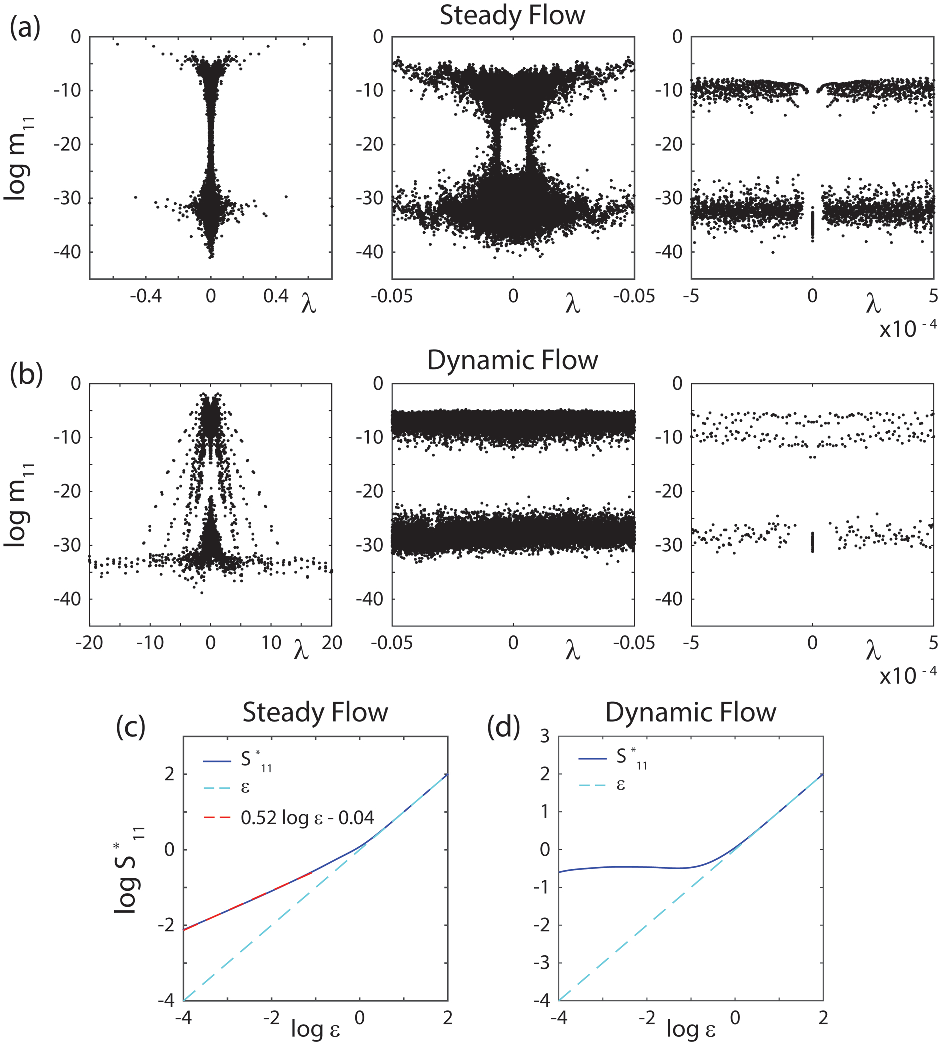
\includegraphics[scale=0.75]{Figure1_Spectral_Measures_Effective_Diffusivities}} 
\caption{%
  Computations of spectral measures and effective diffusivities for
  steady and dynamic flows. The spectral measure $\mu_{11}$ associated
  with the flow in~\eqref{eq:tdcell} are displayed for (a) the steady
  setting and (b) the dynamic setting with the associated effective
  diffusivity $\Sm^*_{11}$ displayed in (c) and (d), respectively. In
  the steady case (a), the 
  limit point of the measure near $\lambda=0$ has small measure mass with
  $m_{11}\lesssim10^{-30}$, leading to the asymptotic behavior
  $\Sm^*_{11}\sim\varepsilon^{1/2}$ for $\varepsilon\ll1$, displayed in (c). In the dynamic case
  (b), the significant measure mass $m_{11}\gtrsim10^{-10}$
  near $\lambda=0$ leads to the asymptotic behavior
  $\Sm^*_{11}\sim1$ for $\varepsilon\ll1$, displayed in (d).
        }
\label{fig:Fig1_Spect_Meas_Eff_Diffus}
\end{figure}
%


In summary, our numerical method is the following. Create the matrices
$\Bm$ and $\Cm$ according to equation~\eqref{eq:Fourier_Coef_System}
or~\eqref{eq:Fourier_Coef_System_Steady} and the corresponding
bijective mapping in~\eqref{eq:Bijections}. Compute \emph{all} the
eigenvalues $\lambda_l$ and eigenvectors $\vecv_l$ of the symmetric matrix
$\Cm^{-1/2}\Bm\Cm^{-1/2}$. The computed Fourier coefficients of the
eigenfunction $\varphi_l$ are given by 
$\veca_l=\Cm^{-1/2}\vecv_l$. The eigenvalues associated with the
discrete component of the spectral measure shown in
equation~\eqref{eq:disc_Integral_Rep_kappa*} are given by $\lambda_l$, while
the spectral measure weights $m_{jk}(l)=\langle u_j,\varphi_l\rangle\,\overline{\langle u_k,\varphi_l\rangle}$
in~\eqref{eq:Spec_Weights} are determined by the vector $\veca_l$ via
equation~\eqref{eq:Inner_Products_2D}
or~\eqref{eq:Inner_Products_2D_Steady}.      



In our computations, we used for the steady case $N=150$, yielding
matrices of size $(2N+1)^2-1=90,600$, while in the dynamic case we used
$N=20$, yielding matrices of size $(2N+1)[(2N+1)^2-1]=68,880$. The
eigenvalues and eigenvectors of the symmetric matrix 
$\Cm^{-1/2}\Bm\Cm^{-1/2}$ were computed using the Matlab function
\emph{eig()} and used to compute the discrete spectral measure and
effective diffusivity. The stability of the computations are measured in terms
of the condition numbers $\mathcal{K}_l$ of the eigenvalues $\lambda_l$,
which are the reciprocals of the cosines of the angles between the
left and right eigenvectors. Eigenvalue condition numbers close to 1
indicate a stable computation. Our eigenvalue computations are
extremely stable with $\max_l|1-\mathcal{K}_l|\sim10^{-14}$, which were
computed using the Matlab function \emph{condeig()}.



Displayed in \figref{fig:Fig1_Spect_Meas_Eff_Diffus} are our
computations of the discrete component of the spectral measure
$\d\mu_{11}(\lambda)=\sum_lm_{11}(l)\delta_{\lambda_l}(\d\lambda)$ associated with the fluid
velocity field $\vecu$ shown in equation~\eqref{eq:tdcell}, for (a)
the steady $(\theta=0)$ and (b) the dynamic $(\theta=1)$ settings. Here, the
spectral weights $m_{11}(l)=|\langle u_1,\varphi_l\rangle|^2$ are determined by
equations~\eqref{eq:Inner_Products_2D_Steady}
and~\eqref{eq:Inner_Products_2D}, respectively.  Consistent with the
symmetries of the flows~\cite{Biferale:PF:2725}, we have
$\mu_{11}=\mu_{22}$, while $\Real\mu_{12}=0$ and $\Imag\mu_{12}=0$, up to
numerical accuracy and finite size effects.




For the 2D steady cell
flow in~\eqref{eq:tdcell} with $\theta=0$, it is
known~\cite{Fannjiang:1994:SIAM_JAM:333,Novikov:2005:CPAM:867} that
$\Sm^*_{11}\sim\varepsilon^{1/2}$ for $\varepsilon\ll1$. Our computation of $\Sm^*_{11}$
displayed in \figref{fig:Fig1_Spect_Meas_Eff_Diffus}(c) is in
excellent agreement with this result, with a computed critical
exponent of $\approx0.52$ having an error of only $4\%$ relative to its true
value $0.5$. Reducing $N$ from 150 to 100 changes the value of the
critical exponent by less than $0.0015$, indicating that the value of
$N=150$ is sufficiently large. In this steady setting, the underlying
operator $(-\Delta)^{-1}[\vecu_1\bcdot\bnabla]$ is
compact~\cite{Bhattacharya:AAP:1999:951} and therefore has 
bounded, discrete spectrum away from the spectral origin, with a limit
point at $\lambda=0$~\cite{Stakgold:BVP:2000}. The limit point behavior of  
the measure $\mu_{11}$ can be seen in the rightmost panel of
\figref{fig:Fig1_Spect_Meas_Eff_Diffus}(a). The decay of $\Sm^*_{11}$
for vanishing $\varepsilon$ is due to the magnitude of the measure masses
$m_{11}(l)\lesssim10^{-30}$ for $|\lambda_l|\ll1$, with a significant \emph{spectral
  gap} near the limit point. The rigorous
result~\cite{Fannjiang:1994:SIAM_JAM:333,Novikov:2005:CPAM:867} $\Sm^*_{11}\sim\varepsilon^{1/2}$ as
$\varepsilon\to0$ reveals that the spectrum of the operator
$(-\Delta)^{-1}[\vecu_1\bcdot\bnabla]$ at $\lambda=0$ is either
continuous or it is discrete with zero mass,
otherwise $\Sm^*_{11}$ would diverge as $\varepsilon\to0$.  



In contrast, as shown in \figref{fig:Fig1_Spect_Meas_Eff_Diffus}(b),
the spectral measure $\mu_{11}$ associated with the time-dependent fluid
velocity field in~\eqref{eq:tdcell}, with $\theta=1$, has significant
values of $m_{11}(l)$ near the spectral origin, with
$m_{11}(l)\gtrsim10^{-10}$ more than \emph{20 orders} of magnitude greater
than  that of the steady flow. A limit point behavior in the measure
$\mu_{11}$ near $\lambda=0$ can be seen in the rightmost panel of
\figref{fig:Fig1_Spect_Meas_Eff_Diffus}(b).  It is interesting to note
that the support $supp\,\mu_{11}$ of the measure $\mu_{11}$ increases with
$N$ and satisfies
$supp\,\mu_{11}\subset[-N,N]$ for all values of $N$ investigated, which
suggests that $supp\,\mu_{11}$ becomes an unbounded set
as $N\to\infty$. This is consistent with the unboundedness of the
self-adjoint operator $M=-\imath(-\Delta)^{-1}(\partial_t-\vecu\bcdot\bnabla)$. Due to
the significant mass of the measure 
near the spectral origin and its uniform nature, as shown in the
center panel of 
\figref{fig:Fig1_Spect_Meas_Eff_Diffus}(b), the effective diffusivity
has an $O(1)$ behavior, $\Sm^*_{11}\sim1$ for $\varepsilon\ll1$, as shown in
\figref{fig:Fig1_Spect_Meas_Eff_Diffus}(d). This is consistent with 
numerical computations of $\Sm^*_{11}$ using alternate 
methods~\cite{Biferale:PF:2725}. This $O(1)$ behavior of $\Sm^*_{11}$
has been attributed to Lagrangian chaos exhibited by the
flow in~\eqref{eq:tdcell}~\cite{Biferale:PF:2725,ZCX_2015}. This
phenomenon is called \emph{residual diffusion} since the chaotic
mixing of the flow gives rise to large scale macroscopic transport
even in the absence of molecular diffusion, $\varepsilon\to0$. 



% %\newpage

% redefine the command that creates the equation no.
  \setcounter{equation}{1}  % reset equation counter
  \setcounter{section}{0}  % reset section counter
  \renewcommand{\theequation}{A-\arabic{equation}} 
\renewcommand{\thesection}{A-\arabic{section}}

\appendix
%
% \section{Appendix}\label{sec:Appendix}
% %

\section{Spectral theory of unbounded self-adjoint operators in
  Hilbert space} \label{app:Spectral_Theory}    
%
The theory of \emph{unbounded} operators in Hilbert
space was developed largely by John von Neumann and Marshall H. Stone. It
is considerably more technical and challenging than the theory of bounded
operators, as unbounded operators do not form an algebra, nor even a
linear space, because each one is defined on its own domain. In this
section, we review the spectral theory for such operators and, in
particular, the celebrated \emph{spectral theorem} for self-adjoint
operators~\cite{Reed-1980,Stone:64}.


An operator is not determined unless its domain is known. Let $\Phi_1$
and $\Phi_2$ be operators acting on a Hilbert space $\Hs$ with domains
$D(\Phi_1)$ and $D(\Phi_2)$, 
respectively, $D(\Phi_i)\subset\Hs$, $i=1,2$. They are said to be
\emph{identical}, in symbols $\Phi_1\equiv\Phi_2$, if and only if $D(\Phi_1)=D(\Phi_2)$
and $\Phi_1 f=\Phi_2 f$ for every $f$ of their common domain. They are said
to be \emph{equal} in 
the set $\mathscr{S}$, in symbols $\Phi_1=\Phi_2$, if and only if
$\mathscr{S}\subseteq D(\Phi_1)\cap D(\Phi_2)$ and $\Phi_1 f=\Phi_2 f$ for every
$f\in\mathscr{S}$. The operator $\Phi_2$ is said to be an \emph{extension}
(\emph{proper extension}) of the operator $\Phi_1$ if $D(\Phi_1)\subseteq D(\Phi_2)$
($D(\Phi_1)\subset D(\Phi_2)$) and the operators $\Phi_2$ and $\Phi_1$ are equal in
$D(\Phi_1)$~\cite{Stone:64}.   


Consider the sesquilinear inner-product $\langle\cdot,\cdot\rangle$ associated with $\Hs$
satisfying $\langle a\psi,b\varphi\rangle=a\,\overline{b}\,\langle\psi,\varphi\rangle$ and
$\langle\psi,\varphi\rangle=\overline{\langle\varphi,\psi\rangle}$ for all $\psi,\varphi\in\Hs$ and $a,b\in\mathbb{C}$, where
$\overline{z}$ denotes complex conjugation of $z\in\mathbb{C}$.
The $\Hs$--inner-product induces a norm $\|\cdot\|$ defined by
$\|\psi\|=\langle\psi,\psi\rangle^{1/2}$. A linear operator $\Phi$ is said to be \emph{closed}
if for every pair of sequences $\{f_n\}$ and $\{\Phi f_n\}$ (with $f_n\in D(\Phi)$)
that converge in the norm $\|\cdot\|$ to the limits $f$ and $h$, then 
$f\in D(\Phi)$ and $\Phi f=h$~\cite{Stone:64}. The (Hilbert space) 
adjoint $\Phi^*$ of $\Phi$ is   
defined by $\langle\Phi\psi,\varphi\rangle=\langle\psi,\Phi^*\varphi\rangle$ for every $\psi\in D(\Phi)$ and $\varphi\in D(\Phi^*)$. The
adjoint $\Phi^*$ of $\Phi$ is uniquely determined when the domain $D(\Phi)$
\emph{determines} $\Hs$, i.e., the smallest closed linear manifold
containing $D(\Phi)$ is the Hilbert space $\Hs$~\cite{Stone:64}. In this
case, $D(\Phi)\subseteq D(\Phi^*)$ and $\Phi^*$ is a closed linear
operator~\cite{Stone:64}. The operator $\Phi$ is said to be
\emph{symmetric} if $\Phi=\Phi^*$. The operator $\Phi$ is said to be
\emph{self-adjoint} if $\Phi\equiv\Phi^*$. A symmetric operator is said to be
\emph{maximal} if it has no proper symmetric extension. A self-adjoint
operator is a maximal symmetric operator~\cite{Stone:64}. 



The operator $\Phi$ is said to be \emph{bounded} (in operator norm) if
$\|\Phi\|=\sup_{\{\psi\in\Hs   \,:\, \|\psi\|=1\}}\|\Phi\psi\|<\infty$. A bounded linear symmetric
operator is self-adjoint if and only if its domain is
$\Hs$~\cite{Stone:64}. Conversely, the Hellinger--Toeplitz theorem
states that, if the operator $\Phi$ satisfies $\langle\Phi\psi,\varphi\rangle=\langle\psi,\Phi\varphi\rangle$ for \emph{every}
$\psi,\varphi\in\Hs$, then $\Phi$ is bounded on
$\Hs$~\cite{Reed-1980,Stone:64}. This indicates that, if $\Phi$ is an
\emph{unbounded} symmetric operator on $\Hs$, then it is self-adjoint
only on a \emph{proper subset} of $\Hs$ that is dense in $\Hs$. 



The spectrum $\Sigma$ of a self-adjoint operator $\Phi$ on a Hilbert space
$\Hs$ is real-valued~\cite{Reed-1980,Stone:64}. If $\Phi$ is also bounded,
then its spectral radius equal to its operator norm
$\|\Phi\|$~\cite{Reed-1980}, i.e., 
%
\begin{align}\label{eq:Spectral_Radius_Phi}
  \Sigma\subseteq[-\|\Phi\|,\|\Phi\|\,].
\end{align}
%
If $\Phi$ is instead unbounded, its spectrum $\Sigma$ can be an unbounded subset of,
or can even coincide with the set of real numbers
$\mathbb{R}$~\cite{Stone:64}.




We now summarize the spectral theorem for self-adjoint
operators (see Theorems 5.9 and  6.1 in~\cite{Stone:64}). Let
$\Phi$ be a fixed self-adjoint operator with spectrum $\Sigma\subseteq\mathbb{R}$ and 
domain $D(\Phi)$ that is dense in $\Hs$. If $\Phi$ is bounded
then we simply take $D(\Phi)\equiv\Hs$. The spectral theorem states that 
there is a one-to-one correspondence between the self-adjoint
operator $\Phi$ and a family of self-adjoint projection operators
$\{Q(\lambda)\}_{\lambda\in\Sigma}$ --- the resolution of the identity --- that
satisfies~\cite{Stone:64} 
%$\lim_{\lambda\to\,\inf{\Sigma}}Q(\lambda)=0$ and $\lim_{\lambda\to\,\sup{\Sigma}}Q(\lambda)=I$~\cite{Stone:64}
%
\begin{align}\label{eq:Res_Identity_limits}
  \lim_{\lambda\to\,\inf{\Sigma}}Q(\lambda)=0, \quad
  \lim_{\lambda\to\,\sup{\Sigma}}Q(\lambda)=I,
\end{align}
%
where $0$ and $I$ denote the null and identity operators on $\Hs$,
respectively. Furthermore, the \emph{complex-valued} function of the
spectral variable $\lambda$ defined by $\mu_{\psi\varphi}(\lambda)=\langle Q(\lambda)\psi,\varphi\,\rangle$ has real,
$\Real\mu_{\psi\varphi}(\lambda)$, and imaginary, $\Imag\mu_{\psi\varphi}(\lambda)$, parts that are
strictly increasing for $\lambda\in\Sigma$ and of bounded variation for all $\psi,\varphi\in
D(\Phi)$~\cite{Stone:64}, where
%
\begin{align}\label{eq:Fns_Bounded_Var}
  \Real\mu_{\psi\varphi}(\lambda)
         &=\frac{1}{2}\left(\mu_{\psi\varphi}(\lambda)+\overline{\mu}_{\psi\varphi}(\lambda)\right),
  \\
  \Imag\mu_{\psi\varphi}(\lambda)
         &=\frac{1}{2\,\imath}\left(\mu_{\psi\varphi}(\lambda)-\overline{\mu}_{\psi\varphi}(\lambda)\right),
  \notag
\end{align}
%
$\imath=\sqrt{-1}$, and $\lambda\in\Sigma$.





By the sesquilinearity of the inner-product and the fact that the
projection operator $Q(\lambda)$ is self-adjoint, the function $\mu_{\psi\varphi}(\lambda)$
satisfies $\mu_{\varphi\psi}(\lambda)=\overline{\mu}_{\psi\varphi}(\lambda)$. Moreover, the function
$\mu_{\psi\psi}(\lambda)$ is real-valued and positive, $\mu_{\psi\psi}(\lambda)=\langle Q(\lambda)\psi,\psi\rangle=\langle
Q(\lambda)\psi,Q(\lambda)\psi\rangle=\|Q(\lambda)\psi\,\|^2\geq0$, hence $\Real\mu_{\psi\psi}(\lambda)=\mu_{\psi\psi}(\lambda)$ and
$\Imag\mu_{\psi\psi}(\lambda)=0$. With each of these strictly increasing functions
of bounded variation, we associate Stieltjes
measures~\cite{Stieltjes:1995,Stone:64,Folland:99:RealAnalysis}  
%
\begin{align}\label{eq:Bounded_Variation}
  &\d\mu_{\psi\varphi}(\lambda)=\d\langle Q(\lambda)\psi,\varphi\rangle, \qquad
  \d\Real\mu_{\psi\varphi}(\lambda)=\d\Real\langle Q(\lambda)\psi,\varphi\rangle,\\  
  &\d\mu_{\psi\psi}(\lambda)=\d\|Q(\lambda)\psi\,\|^2, \qquad
  \hspace{0.2em}
  \d\Imag\mu_{\psi\varphi}(\lambda)=\d\Imag\langle Q(\lambda)\psi,\varphi\rangle,
  \notag
\end{align}
%
which we will denote by $\mu_{\psi\psi}$, $\mu_{\psi\varphi}$, $\Real\mu_{\psi\varphi}$, and
$\Imag\mu_{\psi\varphi}$. We stress that $\mu_{\psi\psi}$ is a positive measure, $\mu_{\psi\varphi}$
is a complex measure, while $\Real\mu_{\psi\varphi}$ and $\Imag\mu_{\psi\varphi}$ are signed
measures~\cite{Stieltjes:1995,Stone:64}.  



The spectral theorem also provides an operational calculus in Hilbert
space which yields powerful integral representations involving the
Stieltjes measures shown in
equation~\eqref{eq:Bounded_Variation}. A summary of the relevant
details are as   
follows. Let $F(\lambda)$ and $G(\lambda)$ be arbitrary complex-valued functions
and denote by $\Ds(F)$ the set of all $\psi\in D(\Phi)$ such that
$F\in L^2(\mu_{\psi\psi})$, i.e., $F$ is square integrable on the set
$\Sigma$ with respect to the \emph{positive} measure $\mu_{\psi\psi}$, and similarly define
$\Ds(G)$. Then $\Ds(F)$ and $\Ds(G)$ are linear manifolds and there
exist linear operators denoted by $F(\Phi)$ and $G(\Phi)$ with domains
$\Ds(F)$ and $\Ds(G)$, respectively, which are defined in terms of the
following Radon--Stieltjes integrals~\cite{Stone:64}  
%
\begin{align}\label{eq:Spectral_Theorem}
  \langle F(\Phi)\psi,\varphi\rangle&=\int_{-\infty}^\infty F(\lambda)\,\d\mu_{\psi\varphi}(\lambda), \qquad
  \hspace{1em}
  \forall \, \psi\in\mathscr{D}(F), \ \varphi\in D(\Phi),  
  \\
  \langle F(\Phi)\psi,G(\Phi)\varphi\rangle&=\int_{-\infty}^\infty F(\lambda)\overline{G}(\lambda)\,\d\mu_{\psi\varphi}(\lambda),
  \quad
  \forall \, \psi\in\mathscr{D}(F), \ \varphi\in\mathscr{D}(G),
  \notag
\end{align}
%
where the integration in~\eqref{eq:Spectral_Theorem} is over the
spectrum $\Sigma$ of $\Phi$~\cite{Reed-1980,Stone:64}.



The mass $\mu^0_{\psi\varphi}=\int_{-\infty}^\infty\d\mu_{\psi\varphi}(\lambda)$ of the
Stieltjes measure $\mu_{\psi\varphi}$ satisfies~\cite{Stone:64}
$\mu^0_{\psi\varphi}=\lim_{\lambda\to\sup\Sigma}\mu_{\psi\varphi}(\lambda)-\lim_{\lambda\to\inf\Sigma}\mu_{\psi\varphi}(\lambda)$. Consequently,
equation~\eqref{eq:Res_Identity_limits} and the Cauchy-Schwartz
inequality yield
% 
\begin{align}\label{eq:Mass_General}
  \mu^0_{\psi\varphi}=\int_{-\infty}^\infty\d\langle Q(\lambda)\psi,\varphi\,\rangle=\langle\psi,\varphi\rangle,
  \qquad
  |\mu^0_{\psi\varphi}|\leq\|\psi\|\,\|\varphi\|<\infty.
\end{align}
%
Equation~\eqref{eq:Mass_General} demonstrates that the measures
in~\eqref{eq:Bounded_Variation} are \emph{finite measures}, i.e., they
have bounded mass~\cite{Stone:64}.



The operators encountered in the ensuing appendices are
\emph{skew-symmetric} operators, which are and example of normal
operators. 
Equation~\eqref{eq:Spectral_Theorem} can be generalized, holding with
suitable notational changes, for \emph{maximal normal
  operators}~\cite{Stone:64}. Such a normal operator $\Nb$ with domain
$D(\Nb)$ dense in $\Hs$ commutes with its adjoint $\Nb^*$, i.e., 
$\Nb\Nb^*=\Nb^*\Nb$, and can be decomposed as $\Nb=\Phi_1+\imath\Phi_2$, where
$\Phi_1$ and $\Phi_2$ are self-adjoint and commute. The spectrum of the
normal operator $\Nb$ is 
a (possibly unbounded) subset of $\mathbb{C}$~\cite{Stone:64}. A
special case of a normal operator is a \emph{skew-adjoint} operator
satisfying $\Nb^*=-\Nb$. It can be decomposed as $\Nb=\imath\Phi_2$ and since
$\Phi_2$ is self-adjoint having purely real spectrum, the skew-adjoint
operator $\Nb=\imath\Phi_2$ has purely imaginary
spectrum~\cite{Stone:64}. Consequently, given such a maximal
skew-adjoint operator, one can focus attention on the self-adjoint
operator $\Phi_2=-\imath\Nb$ without having to resort to the more notationally
complicated spectral theory of normal operators.





The signed measures $\Real\mu_{\psi\varphi}$ and $\Imag\mu_{\psi\varphi}$ shown
in~\eqref{eq:Bounded_Variation} arise naturally when considering 
a maximal skew-adjoint operator $\Nb=\imath\Phi$, where $\Phi$ is
self-adjoint. This can be illustrated by considering some special
cases that arise naturally in
\secref{app:Hilbert_Resolvent_Integral_Reps} below. Consider the
functional $\langle F(\Nb)\psi,G(\Nb)\varphi\rangle$ involving 
\emph{real-valued} Hilbert space members $F(\Nb)\psi$ and $G(\Nb)\varphi$, so
that $\langle F(\Nb)\psi,G(\Nb)\varphi\rangle=\langle G(\Nb)\varphi,F(\Nb)\psi\rangle\in\mathbb{R}$ and, in
particular, 
%$\langle F(\Nb)\psi,G(\Nb)\varphi\rangle=(\langle F(\Nb)\psi,G(\Nb)\varphi\rangle+\langle G(\Nb)\varphi,F(\Nb)\psi\rangle)/2$.
%
\begin{align}\label{eq:Real_Val_Functional}
  \langle F(\Nb)\psi,G(\Nb)\varphi\rangle=\frac{1}{2}(\langle F(\Nb)\psi,G(\Nb)\varphi\rangle+\langle G(\Nb)\varphi,F(\Nb)\psi\rangle).
\end{align}
%
Now consider the special cases $F(\Nb)=G(\Nb)$ and $F(\Nb)=\Nb G(\Nb)$,
i.e., $F(\imath\lambda)=G(\imath\lambda)$ and $F(\imath\lambda)=\imath\lambda G(\imath\lambda)$ in
equation~\eqref{eq:Spectral_Theorem}, respectively. 
From equations~\eqref{eq:Spectral_Theorem}
and~\eqref{eq:Real_Val_Functional}, the identities
$\Real z=(z+\overline{z})/2$ and $\Imag z=(z-\overline{z})/(2\imath)$, and
the linearity properties~\cite{Stone:64} of Stieltjes-Radon integrals
with respect to the functions $\mu_{\psi\varphi}(\lambda)$ and $\overline{\mu}_{\psi\varphi}(\lambda)$,
we have
%
\begin{align}\label{eq:Real_Imag_mu_Reps}
  \langle G(\Nb)\psi,G(\Nb)\varphi\rangle&=\int_{-\infty}^\infty|G(\imath\lambda)|^2\,\d\Real\mu_{\psi\varphi}(\lambda),
  \\
   \langle\Nb G(\Nb)\psi,G(\Nb)\varphi\rangle&=-\int_{-\infty}^\infty\lambda\,|G(\imath\lambda)|^2\,\d\Imag\mu_{\psi\varphi}(\lambda).
   \notag
\end{align}
%




An important property of a self-adjoint operator $\Phi$ which will be
used later is that its domain $D(\Phi)$ comprises those and only those
elements $\psi\in\Hs$ such that the Stieltjes integral
$\int_{-\infty}^\infty\lambda^2\,\d\mu_{\psi\psi}(\lambda)$ is convergent. When $\psi\in D(\Phi)$ the element
$\Phi\psi$ is determined by the relations~\cite{Stone:64}      
%
\begin{align}\label{eq:X_Q_Correspondence}
  \langle\Phi\psi,\varphi\rangle=\int_{-\infty}^\infty\lambda\,\d\mu_{\psi\varphi}(\lambda), \qquad
  \|\Phi\psi\|^2=\int_{-\infty}^\infty\lambda^2\,\d\mu_{\psi\psi}(\lambda),
\end{align}
%
where $\varphi$ is an arbitrary element in $D(\Phi)$~\cite{Stone:64}. In fact,
this determines the one-to-one correspondence between the
self-adjoint operator $\Phi$ and its resolution of the identity
$Q(\lambda)$~\cite{Stone:64}. 





\section{Time derivative as a maximal normal
  operator}\label{app:Time_Derivative}
%
A key example of an unbounded operator is the time derivative
$\partial_t$ acting on the space $L^2(\Tc)$ of Lebesgue measurable functions
that are also square integrable on the interval $\Tc=[0,T]$, say. The
unboundedness of $\partial_t$ as an operator on $L^2(\Tc)$ can be 
understood by considering the orthonormal set of functions
$\{\varphi_n\}\subset L^2(\Tc)$ defined by     
%
\begin{align}\label{eq:Orthonormal}
  \varphi_n(t)=\beta\sin(n\pi t/T), \quad
  \beta=\sqrt{2/T},
  \qquad
  \langle\varphi_n,\varphi_m\rangle_2=\delta_{nm},
  %\quad
  %n,m\in\mathbb{N},
\end{align}
%
where $n,m\in\mathbb{N}$ and $\langle\cdot,\cdot\rangle_2$ denotes the sesquilinear
$L^2(\Tc)$--inner-product. It follows from $\partial_t\varphi_n=(n\pi\beta/T)\cos(n\pi t/T)$
and $\|\partial_t\varphi_n\|^2=(n\pi/T)^2$, that the norm of the members of the set
$\{\partial_t\varphi_n\}$ grows arbitrarily large as $n\to\infty$. This clearly demonstrates
the unboundedness of the operator $\partial_t$ with domain $L^2(\Tc)$.





When one also imposes periodic or Dirichlet boundary conditions,
simple integration by parts demonstrates that the operator $\partial_t$ is
\emph{skew-symmetric} on $L^2(\Tc)$ so that $-\imath\partial_t$ is symmetric with
respect to the sesquilinear inner-product $\langle\cdot,\cdot\rangle_2$. We now identify an
everywhere dense subset of $L^2(\Tc)$ on which $-\imath\partial_t$ is a bounded
linear self-adjoint operator~\cite{Reed-1980,Stone:64}. Consider the
class $\As_{\Tc}$ of all functions $\psi\in L^2(\Tc)$ such that $\psi(t)$ is
\emph{absolutely continuous}~\cite{Royden:1988:RA} on the interval
$\Tc$ and has a derivative $\psi^{\,\prime}(t)$ belonging to $L^2(\Tc)$,
i.e.,~\cite{Stone:64,Royden:1988:RA}     
%
\begin{align}\label{eq:AC_L2}
  \As_{\Tc}=
     \left\{
       \psi\in L^2(\Tc) \ \Big| \ \psi(t)=c+\int_0^tg(s)ds,
       \quad  g\in L^2(\Tc)
     \right\},
\end{align}
%
where the constant $c$ and function $g(s)$ are
arbitrary. Now, consider the set $\tilde{\As}_{\Tc}$ of all
functions $\psi\in\As_{\Tc}$ that satisfy the periodic boundary condition
$\psi(0)=\psi(T)$, i.e. functions $\psi$ satisfying the properties of 
equation~\eqref{eq:AC_L2} with $c$ arbitrary and
$\int_0^Tg(s)ds=0$. In order to help clarify the ideas that were
discussed in~\appref{app:Spectral_Theory} in terms of an abstract  
Hilbert space $\Hs$, we also consider the set $\hat{\As}_{\Tc}$ of all
functions $\psi\in\As_{\Tc}$ that satisfy the Dirichlet boundary condition
$\psi(0)=\psi(T)=0$, i.e. functions $\psi$ satisfying the properties of
equation~\eqref{eq:AC_L2} with $c=0$ and $\int_0^Tg(s)ds=0$. More
concisely,  
%
\begin{align}\label{eq:AC_BC}
  \tilde{\As}_{\Tc}&=\{\psi\in\As_{\Tc} \,|\, \psi(0)=\psi(T)\},
  \\
  \hat{\As}_{\Tc}&=\{\psi\in\As_{\Tc} \,|\, \psi(0)=\psi(T)=0\}.
  \notag
\end{align}
%
These function spaces satisfy
$\hat{\As}_{\Tc}\subset\tilde{\As}_{\Tc}\subset\As_{\Tc}$ and are each everywhere
dense in $L^2(\Tc)$~\cite{Stone:64}. Let the operators $B$,
$\tilde{B}$, and $\hat{B}$ be identified as $-\imath\partial_t$ with domains
$\As_{\Tc}$, $\tilde{\As}_{\Tc}$, and $\hat{\As}_{\Tc}$,
respectively. Then, $\hat{B}$ is a closed linear symmetric operator
with the adjoint $\hat{B}^*\equiv B$, and the operator $\tilde{B}$ is a
\emph{self-adjoint} extension of $\hat{B}$~\cite{Stone:64}. In
symbols, this means that $\tilde{B}=\tilde{B}^*$ on
$\tilde{\As}_{\Tc}$ and
$D(\tilde{B})=D(\tilde{B}^*)=\tilde{\As}_{\Tc}$,
i.e., $\tilde{B}\equiv\tilde{B}^*$ on $\tilde{\As}_{\Tc}$. This establishes
that the operator $-\imath\partial_t$ with domain $\tilde{\As}_{\Tc}$ is
self-adjoint, hence $\partial_t$ is a maximal skew-symmetric (normal)
operator on $\tilde{\As}_{\Tc}$. The operator $\imath\partial_t$ on
$\tilde{\As}_{\Tc}$ has a simple point spectrum, consisting of
eigenvalues $\lambda=2n\pi/T$, $n\in\mathbb{Z}$, with corresponding
eigenfunctions $\exp(\imath\,2n\pi t/T)$~\cite{Stone:64}.





\section{Hilbert spaces, resolvents, and integral representations of the effective diffusivity}
\label{app:Hilbert_Resolvent_Integral_Reps} 
%
In this section we provide a spectral theory of effective
diffusivities for space-time periodic flows. In particular, two
different approaches to the effective parameter problem for
advection-diffusion were proposed
in~\cite{Pavliotis:PHD_Thesis,Bhattacharya:AAP:1999:951}  
and~\cite{Avellaneda:PRL-753,Avellaneda:CMP-339} for
\emph{time-independent} flows. We generalize these results to the
setting of \emph{time-dependent}, chaotic flows. Specifically, we
formulate rigorous mathematical 
frameworks for each approach which provide Stieltjes integral
representations for both the symmetric $\Sm^*$ and antisymmetric
$\Am^*$ parts of the effective diffusivity tensor $\Dm^*$ for
space-time periodic flows, involving a spectral measure of an
\emph{unbounded} self-adjoint operator. In~\appref{app:Scalar_Fields}
we generalize the approach proposed
in~\cite{Pavliotis:PHD_Thesis}, 
while in~\appref{app:Curl_Free_Fields} we generalize the approach
proposed
in~\cite{Avellaneda:PRL-753,Avellaneda:CMP-339}. In~\appref{app:Isometric_Correspondence}
we establish that the two approaches are equivalent, using the
one-to-one correspondence between a self-adjoint operator and its
resolution of the identity~\cite{Stone:64}, discussed in the paragraph
containing equation~\eqref{eq:X_Q_Correspondence}.   



\subsection{Scalar fields and effective diffusivity}\label{app:Scalar_Fields}
%
In this section we consider a formulation of the effective parameter
problem for advection-diffusion that was first proposed
in~\cite{Pavliotis:PHD_Thesis,Bhattacharya:AAP:1999:951} for
\emph{time-independent} flows. In particular, we provide an abstract
Hilbert space formulation of the effective parameter problem that
generalizes the formulation in~\cite{Pavliotis:PHD_Thesis} to include
space-time periodic fluid velocity fields, with possibly chaotic
dynamics. 



To fix ideas, consider the following sets $\Tc=[0,T]$ and 
$\Vc=\otimes_{j=1}^d[0,L]$ which  define the space-time period cell
$\Tc\times\Vc$. Now consider the Hilbert spaces
$L^2(\Tc)$ and $L^2(\Vc)$ of Lebesgue measurable scalar functions over
the complex field $\mathbb{C}$ that are also square
integrable~\cite{Folland:99:RealAnalysis}. Define the associated
Hilbert spaces $\Hs_{\Tc}$, $\Hs_{\Vc}$, and
$\Hs_{\Tc\Vc}=\Hs_{\Tc}\otimes\Hs_{\Vc}$ of periodic functions, where  
%
\begin{align}\label{eq:Hilbert_Spaces_scalar}  
  \Hs_{\Tc}&=\big\{\psi\in L^2(\Tc) \, | \, \psi(t)=\psi(t+T)\big\},
  \\
  \Hs_{\Vc}&
  =\big\{\psi\in L^2(\Vc) \, | \, \psi(\vecx)=\psi(\vecx+L\vece_j), \ j=1,\ldots,d\big\},
  \notag
\end{align}
%
and the $\vece_j$ are standard basis
vectors. More specifically, denote time average over $\Tc$ by
$\langle\cdot\rangle_{\Tc}$, space average over $\Vc$ by $\langle\cdot\rangle_{\Vc}$, and space-time
average over $\Tc\times\Vc$ by $\langle\cdot\rangle$. The space-time average $\langle\cdot\rangle$,
induces a sesquilinear inner-product $\langle\cdot,\cdot\rangle$ given by
$\langle\psi,\varphi\rangle=\langle\psi\;\overline{\varphi}\rangle$, with $\langle\varphi,\psi\rangle=\overline{\langle\psi,\varphi\rangle}$. This
$\Hs_{\Tc\Vc}$--inner-product, in turn, induces a norm $\|\cdot\|$ given by
$\|\psi\|=\langle\psi,\psi\rangle^{1/2}$~\cite{Folland:99:RealAnalysis}. The space of
space-time periodic
Lebesgue measurable functions $\Hs_{\Tc\Vc}$ satisfying $\|f\|<\infty$ is a
complete Hilbert space~\cite{Folland:99:RealAnalysis}. Similarly, the
space and time averages, 
$\langle\cdot\rangle_{\Vc}$ and $\langle\cdot\rangle_{\Tc}$, induce sesquilinear inner-products,
$\langle\cdot,\cdot\rangle_{\Vc}$ and $\langle\cdot,\cdot\rangle_{\Tc}$, that induce norms, $\|\cdot\|_{\Vc}$ and
$\|\cdot\|_{\Tc}$, associated with the Hilbert spaces $\Hs_{\Tc}$
and $\Hs_{\Vc}$. 




In equation~\eqref{eq:AC_BC} we defined the space $\tilde{\As}_{\Tc}$ of
absolutely continuous $\Tc$--periodic functions with time derivatives
belonging to $L^2(\Tc)$, which is \emph{not} a Hilbert space but is
instead an everywhere dense subset of the Hilbert space
$\Hs_\Tc$~\cite{Stone:64}. To treat spatial dependence, we define 
the Sobolev space $\Hs^{1,2}_{\Vc}$ which is itself a Hilbert
space~\cite{Bhattacharya:AAP:1999:951,Folland:95:PDEs,McOwen:2003:PDE},             
% 
\begin{align}\label{eq:Sobolev}
  \Hs^{1,2}_{\Vc}=\big\{\psi\in \Hs_{\Vc} \; | \; \|\bnabla\psi\|_{\Vc}<\infty, \ \langle\psi\rangle_{\Vc}=0\big\}.
\end{align}
%
The condition $\langle\psi\rangle_{\Vc}=0$ in~\eqref{eq:Sobolev} is
required to eliminate non-zero constant $\psi$, which satisfies
$\|\bnabla\psi\|_{\Vc}=0$.  
The $\Hs^{1,2}_{\Vc}$--norm $\|\bnabla\cdot\|_{\Vc}$ is induced by the
$\Hs^{1,2}_{\Vc}$--inner-product:
$\|\bnabla\psi\|_{\Vc}=\langle\bnabla\psi\bcdot\bnabla\psi\rangle_{\Vc}^{1/2}$. 
The Sobolev space $\Hs^{1,2}_{\Vc}$  is the closure in the norm
$\|\bnabla\cdot\|_{\Vc}$ of the space $C^2(\Vc)$ of all twice continuously
differentiable functions in $\Hs_{\Vc}$ which are also mean-zero and
$\Vc$--periodic, and all the elements of $\Hs^{1,2}_{\Vc}$ are those elements
of $\Hs_{\Vc}$ which have square integrable gradients on the set
$\Vc$~\cite{Bhattacharya:AAP:1999:951}. Functions in $\Hs^{1,2}_{\Vc}$
need not be differentiable in the classical 
sense. Instead, $f\in\Hs^{1,2}_{\Vc}$ has derivatives $\partial f/\partial x_j\in
L^2(\Vc)$ defined by $\partial f/\partial x_j=\lim_{n\to\infty}\partial f_n/\partial x_j$, where $f_n\in
C^2(\Vc)$ are Cauchy in the norm $\|\bnabla\cdot\|_{\Vc}$, and convergence is
in $L^2(\Vc)$~\cite{McOwen:2003:PDE}. 




Finally, consider the Hilbert
space $\Hs$ and its everywhere dense subset $\Fs$ defined by
%
\begin{align}\label{eq:Function_Space_Scalar}
  \Hs=\Hs_{\Tc}\otimes\Hs^{1,2}_{\Vc}, \qquad
  \Fs=\tilde{\As}_{\Tc}\otimes\Hs^{1,2}_{\Vc}.
  %\Hs=\big\{\psi\in\Hs_{\Tc}\otimes\Hs^{1,2}_{\Vc} \; | \; \langle \psi\rangle=0\big\}, \\
  %\Fs=\big\{\psi\in\tilde{\As}_{\Tc}\otimes\Hs^{1,2}_{\Vc} \; | \; \langle \psi\rangle=0\big\}.
  %\notag
\end{align}
%
We stress that $\tilde{\As}_{\Tc}$ and $\Fs$ are \emph{not} a
complete Hilbert spaces. Instead, they are everywhere dense subsets of
the complete Hilbert spaces $\Hs_{\Tc}$ and $\Hs$, respectively.
Recalling that $\langle\cdot\rangle$ denotes space-time average over $\Tc\times\Vc$ and
$\vecpsi\bcdot\vecvarphi=\vecpsi^T\overline{\vecvarphi}$, 
the sesquilinear  
$\Hs$--inner-product is given by $\langle\psi,\varphi\rangle_{1,2}=\left\langle\bnabla \psi\bcdot\bnabla \varphi \right\rangle$ with associated norm
$\|\cdot\|_{1,2}$ given by $\|\psi\|_{1,2}= \langle|\bnabla \psi|^2\rangle^{1/2}$.
% Since
% $\langle|\partial_t\psi|^2\rangle_{\Tc}<\infty$ for all $\psi\in\tilde{\As}_{\Tc}$ and
% $\langle|\bnabla \psi|^2\rangle_{\Vc}<\infty$ for all $\psi\in\Hs^{1,2}_{\Vc}$, it follows that
% $\|\partial_t\psi\|_{1,2}^2=\langle|\bnabla \partial_t\psi|^2\rangle<\infty$ and $\|\psi\|_{1,2}<\infty$ for all
% $\psi\in\Fs$.
In the case of a 
time-independent fluid velocity field $\vecu=\vecu(\vecx)$ we set 
$\Hs\equiv\Fs\equiv\Hs^{1,2}_{\Vc}$ and $\langle\cdot\rangle=\langle\cdot\rangle_{\Vc}$.  We stress  it is
crutial that $\psi\in\Hs$ satisfy $\langle\psi\rangle_{\Vc}=0$, as required by the
definition of $\Hs^{1,2}_{\Vc}$ in~\eqref{eq:Sobolev}. Otherwise,
$\|\cdot\|_{1,2}=\int_{\Tc\times\Vc}\d t\,\d\vecx\,|\bnabla\cdot|^2$ is not a norm,
since a strictly positive function $\psi(t,\vecx)=\psi(t)$ on $\Tc\times\Vc$
satisfies $\|\psi\|_{1,2}=0$.    





We now use properties of the Hilbert space $\Hs$ to obtain
functional formulas for the symmetric $\Sm^*$ and antisymmetric
$\Am^*$ parts of the effective diffusivity tensor $\Dm^*$ defined in
equations~\eqref{eq:Djk} and~\eqref{eq:Symm_Anti-Symm}, involving the
solution $\chi_j$ of the cell problem in
equation~\eqref{eq:Periodic_Cell_Prob} and a maximal skew-symmetric
operator $A$ on $\Fs$. We then derive from the cell 
problem a resolvent formula for $\chi_j$ involving the operator
$A$. The spectral theorem discussed in~\appref{app:Spectral_Theory}
then yields Stieltjes integral representations for
$\Sm^*$ and $\Am^*$, which are established in
\thmref{thm:Integral_Reps} below. 


Applying the linear operator $(-\Delta)^{-1}$ to both sides of the cell
problem in equation~\eqref{eq:Periodic_Cell_Prob} yields, with
suitable notational changes,
%$(-\Delta)^{-1}u_j=[\varepsilon+(-\Delta)^{-1}(\partial_t-\vecu\bcdot\bnabla)]\chi_j$.
%
\begin{align}\label{eq:Pre_Resolvent_Scalar}
  (-\Delta)^{-1}u_j=(\varepsilon+A)\chi_j,
  \qquad
  A=(-\Delta)^{-1}(\partial_t-\vecu \bcdot\bnabla).
\end{align}
%
%where we have defined $A=(-\Delta)^{-1}(\partial_t-\vecu \bcdot\bnabla)$.
We will discuss the key properties of the operators $(-\Delta)^{-1}$ and
$A$ in more detail below.  Now write the functional $\langle u_j\chi_k\rangle$ in 
equation~\eqref{eq:Djk} as~\cite{Pavliotis:PHD_Thesis}       
%
\begin{align}\label{eq:uj_chik}
  %\langle u_j\chi_k\rangle=
  \langle[(-\Delta)(-\Delta)^{-1}u_j]\,\chi_k\rangle
       =\langle\bnabla(-\Delta)^{-1}u_j\bcdot\bnabla \chi_k\rangle
       =\langle(-\Delta)^{-1}u_j,\chi_k\rangle_{1,2}.
\end{align}
%
This calculation will be justified below. Substituting the  
formula in~\eqref{eq:Pre_Resolvent_Scalar} for $(-\Delta)^{-1}u_j$ 
into equation~\eqref{eq:uj_chik} yields
equation~\eqref{eq:Eff_Diffusivity_Sobolev}, which provides functional
formulas for the components
$\Sm^*_{jk}$ and $\Am^*_{jk}$, $j,k=1,\ldots,d$, of $\Sm^*$ and $\Am^*$.
Equation~\eqref{eq:Pre_Resolvent_Scalar}   
leads to the resolvent formula shown
in~\eqref{eq:Resolvent_Rep_Scalar}.  
From equations~\eqref{eq:Eff_Diffusivity_Sobolev}
and~\eqref{eq:Resolvent_Rep_Scalar} we have the functional formulas
for $\Sm^*_{jk}$ and $\Am^*_{jk}$ shown in 
equation~\eqref{eq:Eff_Diff_Resolvent_Sobolev} involving the resolvent
of the operator $A$. The following theorem establishes the 
Stieltjes integral representations equation
in~\eqref{eq:Integral_Rep_kappa*} for these functional formulas of
$\Sm^*_{jk}$ and $\Am^*_{jk}$.  



%
\begin{theorem}\label{thm:Integral_Reps}
  The operator $A=(-\Delta)^{-1}(\partial_t-\vecu\bcdot\bnabla)$ is a maximal
  (skew-symmetric) normal operator on the function space $\Fs$, hence
  $M=-\imath A$ is self-adjoint on $\Fs$. Let $Q(\lambda)$ be the resolution of
  the identity in one-to-one correspondence with $M$. Define the
  complex valued function $\mu_{jk}(\lambda)=\langle Q(\lambda)g_j,g_k\rangle_{1,2}$,
  $j,k=1,\ldots,d$, where $g_j=(-\Delta)^{-1}u_j$. Consider the positive measure
  $\mu_{kk}$ and the signed measures $\Real\mu_{jk}$ and $\Imag\mu_{jk}$
  associated with $\mu_{jk}(\lambda)$, introduced
  in~\eqref{eq:Fns_Bounded_Var}.  Then, for $\chi_j\in\Fs$,
  $u_j\in\tilde{\As}_{\Tc}\otimes(\Hs_{\Vc}\cap L^r(\Vc))$, $2<r\leq\infty$, satisfying
  $\langle u_j\rangle_{\Vc}=0$, and all $0<\varepsilon<\infty$, the functional formulas for $\Sm^*_{jk}$
  and $\Am^*_{jk}$ in~\eqref{eq:Eff_Diff_Resolvent_Sobolev} have the
  Radon--Stieltjes integral representations shown in
  equation~\eqref{eq:Integral_Rep_kappa*}.     
% 
\end{theorem}
%


Before proving \thmref{thm:Integral_Reps}, we justify the calculation 
in equation~\eqref{eq:uj_chik} and discuss key properties of the
linear operator $(-\Delta)^{-1}$ and the function $u_j$ on the right side
of the cell problem in~\eqref{eq:Periodic_Cell_Prob}. Recall the 
discussion in \secref{sec:Mean_Flow} regarding the properties of the
effective diffusivity tensor $\Dm^*$ when the fluid velocity field
$\vecu$ has a large scale mean flow $\vecu_0$. Specifically, recall
that the cell problem is analogous to
equation~\eqref{eq:Periodic_Cell_Prob}, which holds for a mean-zero
velocity field, $\vecu_0\equiv0$. Moreover, the function $u_j$ on the right
side of the cell problem is mean-zero, $\langle u_j\rangle=0$, regardless of
whether the strength of $\vecu_0$ is
weak~\cite{Majda:Kramer:1999:book,Pavliotis:PHD_Thesis} or
comparable~\cite{Pavliotis:PHD_Thesis} to the periodic fluctuations,
e.g. $u_j$ is replaced by the $j$th component of the mean-zero vector
field $\vecu-\vecu_0$.  


Using the $\Hs$--inner-product to obtain Stieltjes integral
representations for $\Dm^*$ requires the function $u_j$ to mean-zero
in space alone, $\langle u_j\rangle_{\Vc}=0$. In particular, in the proof of
\thmref{thm:Integral_Reps} below, we 
show it is required that $(-\Delta)^{-1}u_j\in\Fs$, where
$\Fs=\tilde{\As}_{\Tc}\otimes\Hs^{1,2}_{\Vc}$. Recall in the definition of
$\Hs^{1,2}_{\Vc}$ in~\eqref{eq:Sobolev} we required that
$\psi\in\Hs^{1,2}_{\Vc}$ satisfy $\langle\psi\rangle_{\Vc}=0$. We 
therefore require $\langle(-\Delta)^{-1}u_j(t,\cdot)\rangle_{\Vc}=0$ for almost all
$t\in\Tc$. Since the Laplacian $\Delta$ maps $\Vc$--periodic functions to
\emph{mean-zero} $\Vc$--periodic functions, in the present context,
the domain of the operator $(-\Delta)^{-1}$ is mean-zero $\Vc$--periodic
functions. We therefore require $\langle u_j(t,\cdot)\rangle_{\Vc}=0$ for almost all
$t\in\Tc$. Conversely, when $\psi$ is mean-zero $\Vc$--periodic then
$(-\Delta)^{-1}\psi$ is also mean-zero $\Vc$--periodic. 



The result of \lemref{lem:A_bounded} below is also central to the
proof of \thmref{thm:Integral_Reps}. There, we require
$u_j\in\tilde{\As}_{\Tc}\otimes(\Hs_{\Vc}\cap L^r(\Vc))$ for $2<r\leq\infty$. This property,
$\langle u_j(t,\cdot)\rangle_{\Vc}=0$ for almost all $t\in\Tc$, 
$\tilde{\As}_{\Tc}\otimes(\Hs_{\Vc}\cap L^r(\Vc))\subset L^2(\Tc\times\Vc)$, and the
Fubini-Tonelli theorem  imply $\langle u_j\rangle=0$. We stress it is 
\emph{not} necessary that $\langle u_j(\cdot,\vecx)\rangle_{\Tc}=0$ for almost all
$\vecx\in\Vc$. The fluid velocity
field $\vecu$ in equation \eqref{eq:tdcell} is such an example,
satisfying $\langle\vecu\rangle_{\Vc}=0$ and $\langle\vecu\rangle=0$ but
$\langle\vecu\rangle_{\Tc}=(\cos{y},\cos{x})\not\equiv0$. The condition $\langle
u_j\rangle_{\Vc}=0$, rules out functions of the form $u_j(t,\vecx)=u_j(t)$
or even $u_j(t,\vecx)=f(t,\vecx)+h(t)$ with $\langle f\rangle_{\Vc}=0$.


\textbf{In summary}, the properties we require the function $u_j$ on
the right side of equation~\eqref{eq:Periodic_Cell_Prob} to have are:
$u_j$ is $\Tc\times\Vc$--periodic, $u_j\in\tilde{\As}_{\Tc}\otimes(\Hs_{\Vc}\cap
L^r(\Vc))$ for $2<r\leq\infty$, $\langle(-\Delta)^{-1}u_j(t,\cdot)\rangle_{\Vc}=0$ for almost all
$t\in\Tc$, and $\langle u_j(t,\cdot)\rangle_{\Vc}=0$ for almost all $t\in\Tc$ (implying
that $u_j$ is mean-zero on $\Tc\times\Vc$, $\langle u_j\rangle=0$).    






We now discuss more key properties of the operator $(-\Delta)^{-1}$ and
justify the calculation in equation~\eqref{eq:uj_chik}. The operator is
$(-\Delta)^{-1}$ based on convolution with respect to the Green's function
for the Laplacian, i.e.,
$(-\Delta)^{-1}f(\vecx)=\int_{\Vc}G(\vecx-\vecy)\,f(\vecy)\,\d\vecy$. It is
positive~\cite{Stakgold:BVP:2000}, $G>0$,
symmetric~\cite{Folland:95:PDEs,Stakgold:BVP:2000}  
$G(\vecx-\vecy)=G(\vecy-\vecx)$,
and integrable~\cite{Melnikov:2012:Green,Melnikov2006774,McCann08042001}
%(e.g. see Proposition 0.5 in~\cite{Folland:95:PDEs})
%
\begin{align}\label{eq:Integrable_G}
 \sup_{\vecx\in\Vc} \int_{\Vc}G(\vecx-\vecy)\d\vecy\leq C<\infty.
\end{align}
%
The Green's function $G$ can be constructed~\cite{Melnikov:2012:Green}
in terms of the eigenvalues $\lambda_{\veck}$ and orthonormal eigenfunctions
$\phi_{\veck}(\vecx)$ of the operator $-\Delta$ with periodic boundary
conditions on $\Vc$, $G(\vecx-\vecy)=\sum_{\veck\in\mathbb{Z}^d\backslash\{0\}}
\phi_{\veck}(\vecx)\,\phi_{\veck}(\vecy)/\lambda_{\veck}$,   
where $\lambda_{\veck}=|\veck|^2$ and
$\{\phi_{\veck}(\vecx)\}=\{\cos(\veck\bcdot\vecx),\sin(\veck\bcdot\vecx)\}$
when $\Vc=[0,2\pi]^d$.
% The set $\{\phi_{\veck}(\vecx)\}$ is an orthonormal
% basis for $\Hs_{\Vc}$~\cite{Folland:99:RealAnalysis}. Since the space
% $\Hs_{\Vc}$ of $\Vc$--periodic functions is a complete Hilbert space,
% the Green's function $G$ is $\Vc$--periodic. In other words, if
% $f_n\in\Hs_{\Vc}$ is a sequence of functions with
% $\lim_{n\to\infty}\|f-f_n\|_{\Vc}$, then the $\Vc$--periodicity of the
% functions $f_n$ implies that
% $\|f(\vecx+L\vece_j)-f(\vecx)\|\leq\|f(\vecx+L\vece_j)-f_n(\vecx+L\vece_j)\|     
% +\|f(\vecx)-f_n(\vecx)\|\to0$ as $n\to\infty$, implying that the limit $f$ is
% $\Vc$--periodic. Letting $f_n$ be the partial sum
% $\sum_{|\veck|\leq n} \phi_{\veck}(\vecx)\,\phi_{\veck}(\vecy)/\lambda_{\veck}$ with $f_n\to G$ 
% shows $G$ is a $\Vc$--periodic function.  



By equation~\eqref{eq:Integrable_G} and Young's
inequality~\cite{Folland:95:PDEs,Folland:99:RealAnalysis}, 
$(-\Delta)^{-1}$ is a bounded operator on $L^p(\Vc)$ for $1\leq p\leq\infty$: if $\psi\in
L^p(\Vc)$ then $(-\Delta)^{-1}\psi\in L^p(\Vc)$ and   
%
\begin{align}\label{eq:Young_Ineq}
  \|(-\Delta)^{-1}\psi\|_p\leq C\|\psi\|_p,
  \quad
  1\leq p\leq\infty,
\end{align}
%
where $\|\cdot\|_p$ denotes the $L^p(\Vc)$--norm and $C$ is defined
in~\eqref{eq:Integrable_G}. Since $\Vc$ is bounded, it has finite
Lebesgue measure $|\Vc|<\infty$. Consequently, we 
have~\cite{Folland:99:RealAnalysis} $L^p(\Vc)\supset L^q(\Vc)$ for all
$0<p<q\leq\infty$ with $\|\psi\|_p\leq\|\psi\|_q\,|\Vc|^{(1/p)-(1/q)}$. In particular,
$L^r(\Vc)\subset L^2(\Vc)$ for all $2<r\leq\infty$. 




The operator $(-\Delta)^{-1}$ satisfies $\langle(-\Delta)(-\Delta)^{-1}f,h\rangle=\langle f,h\rangle$ in the
following weak, distributional
sense~\cite{McOwen:2003:PDE,Folland:95:PDEs}. Let
$f\in\Hs^{1,2}_{\Vc}$ and let $\{ f_n\}$ be a sequence of mean-zero
$\Vc$--periodic functions with $f_n\in C^2(\Vc)$ that is
Cauchy the norm $\langle|\bnabla\cdot|^2\rangle_{\Vc}$ and converges to $f$ in 
$L^2(\Vc)$. Then, for all $h\in\Hs^{1,2}_{\Vc}$ we have  (see
Theorem 1 in Section 4.2 of~\cite{McOwen:2003:PDE})      
%
\begin{align}\label{eq:Weak_Delta_1}
  \langle(-\Delta)(-\Delta)^{-1}f,h\rangle_{\Vc}
  &:=\lim_{n\to\infty}
  \left\langle\int_{\Vc} G(\vecx-\vecy)(-\Delta_y)f_n(\vecy)\d\vecy,h(\vecx)\right\rangle_{\Vc}
  \\\notag
  &=\lim_{n\to\infty}\langle f_n,h\rangle_{\Vc}
  \\\notag
  &=\langle f,h\rangle_{\Vc},
  \notag
\end{align}
%
by the continuity of the
inner-product~\cite{Folland:99:RealAnalysis,Stakgold:BVP:2000} 
and since the boundary terms~\cite{McOwen:2003:PDE}
$\int_{\partial\Vc}[f_n(\vecy)\,\partial G(\vecx-\vecy)/\partial\mathbf{n}_y
-G(\vecx-\vecy)\,\partial f_n(\vecy)/\partial\mathbf{n}_y]\,\d S_y$ vanish by   
periodicity. Here, $\d S_y$ denotes the surface measure on the
boundary $\partial\Vc$ of $\Vc$ and $\partial/\partial\mathbf{n}_y$ is the outward normal
derivative on $\partial\Vc$ equation~\cite{McOwen:2003:PDE}. This justifies
the calculation in~\eqref{eq:uj_chik}. Moreover, integration by parts,
the Cauchy-Schwartz inequality, $|\langle f,g\rangle_{\Vc}|\leq\|f\|_{\Vc}\,\|g\|_{\Vc}$,
and Young's inequality for $p=2$ imply for mean-zero $\psi\in\Hs_{\Vc}$ 
%
\begin{align}\label{eq:L2_to_H1}
  \|\bnabla(-\Delta)^{-1}\psi\|^2_{\Vc}=\langle\bnabla(-\Delta)^{-1}\psi\bcdot\bnabla(-\Delta)^{-1}\psi\rangle_{\Vc}
              %\\
              =|\langle(-\Delta)^{-1}\psi,\psi\rangle_{\Vc}|
              %\notag\\
              \leq C\|\psi\|_{\Vc}^2\,.
              %\notag
\end{align}
%
Therefore, the operator $(-\Delta)^{-1}$ maps mean-zero functions in
$\Hs_{\Vc}$ to $\Hs^{1,2}_{\Vc}$. 









The following lemma will be used in the
proof of \thmref{thm:Integral_Reps} below.
%
\begin{lemma}\label{lem:A_bounded}
%
Assume that the components $u_j$, $j=1,\ldots,d$ of the fluid velocity
field $\vecu$ satisfy $u_j\in\tilde{\As}_{\Tc}\otimes(\Hs_{\Vc}\cap L^r(\Vc))$ for
$2<r\leq\infty$. Then the operator $(-\Delta)^{-1}(\vecu\bcdot\bnabla)$ is bounded
on $\Hs$. Moreover, the following are upper bounds for its operator
norm $\|(-\Delta)^{-1}(\vecu\bcdot\bnabla)\|_{1,2}$ 
%
\begin{align}
  \|(-\Delta)^{-1}(\vecu\bcdot\bnabla)\|_{1,2}
  &\leq\sqrt{C}\sqrt{\sup_{(t,\vecx)\in\Tc\times\Vc}|\vecu|^2},
  ~\text{ when }~ r=\infty,
  \label{eq:Bound_A1}  
  \\
  \|(-\Delta)^{-1}(\vecu\bcdot\bnabla)\|_{1,2}
  &\leq\sqrt{Cd}\;\left[\sum_{j=1}^d\langle|u_j|^r\rangle\right]^{1/r}
  ~\text{ when }~ 2<r<\infty,
  \label{eq:Bound_A2}
\end{align}
%
where the constant $C$ is defined in equation~\eqref{eq:Integrable_G}
and satisfies $0<C<\infty$. 
%
\end{lemma}
%



\textbf{Proof of \lemref{lem:A_bounded}.}\hspace{1ex}
%
Denote by $\|\cdot\|_p$ the $L^p(\Tc\times\Vc)$--norm and let $f\in\Hs$. A
calculation similar to the one given 
in~\eqref{eq:L2_to_H1} and H{\"o}lder's
inequality~\cite{Folland:99:RealAnalysis}, 
$\|f\,g\|_1\leq\|f\|_{p_1}\,\|g\|_{q_1}$, with conjugate exponents
satisfying $(1/p_1)+(1/q_1)=1$ and $1\leq p_1,\,q_1\leq\infty$, yield
%
\begin{align}\label{eq:p1_q1_Bound}
  \|(-\Delta)^{-1}(\vecu\bcdot\bnabla)f\|^2_{1,2}
  %&=\|[(-\Delta)^{-1}(\vecu\bcdot\bnabla f)]\,(\vecu\bcdot\bnabla f)\|_1
  %\\
  &\leq C\|\vecu\bcdot\bnabla f\|_{p_1}\,\|\vecu\bcdot\bnabla f\|_{q_1}\,.
  %\notag
\end{align}
%
When $u_j\in\tilde{\As}_{\Tc}\otimes\Hs_{\Vc}$, for each fixed
$\vecx\in\Vc$ the function $u_j(\cdot,\vecx)$ is absolutely continuous  on
the closed bounded set $\Tc$ and is therefore uniformly
bounded~\cite{Royden:1988:RA,BabyRudin:64}. If we 
also have that $u_j\in\tilde{\As}_{\Tc}\otimes L^r(\Vc)$ for $r=\infty$ then
$u_j(t,\cdot)$ is also uniformly bounded for each $t\in\Tc$ and the fluid
velocity field satisfies $\sup_{(t,\vecx)\in\Tc\times\Vc}|\vecu|^2<\infty$. An
example of such a fluid velocity field is in
equation~\eqref{eq:tdcell}. In this case,
equation~\eqref{eq:p1_q1_Bound} with 
$p_1=q_1=2$ and the Cauchy-Schwartz inequality,
$|\vecu\bcdot\bnabla f|\leq|\vecu|\,|\bnabla f|$, yield the bound given in 
equation~\eqref{eq:Bound_A1}.




We now use equation~\eqref{eq:p1_q1_Bound} to establish the bound
in~\eqref{eq:Bound_A2}, assuming that
$u_j\in\tilde{\As}_{\Tc}\otimes(\Hs_{\Vc}\cap L^r(\Vc))$ for $r\geq2$ and
$r\neq\infty$. Let's first focus 
on the term $\|\vecu\bcdot\bnabla f\|_{p_1}$.  Since $1\leq p_1\leq\infty$,
the function $x^{\,p_1}$ is convex for $x>0$. Therefore, by Jensen's
inequality, $(\sum_{i=1}^d|a_i|/d\,)^{p_1}\leq\sum_{i=1}^d|a_i|^{\,p_1}/d$, and the
triangle inequality we have
%
\begin{align}
  \|\vecu\bcdot\bnabla f\|^{p_1}_{p_1}
  =\left\langle\left|\sum_{i=1}^du_i\,\partial_if\right|^{p_1}\right\rangle
  \leq d^{\,p_1-1}\sum_{i=1}^d\left\langle|u_i|^{p_1}\,|\partial_if|^{p_1} \right\rangle,
\end{align}
%
where $\partial_i$ denotes partial differentiation in the $i$th
direction. H{\"o}lder's inequality, implies that
$\langle|u_i|^{p_1}\,|\partial_if|^{p_1}\rangle\leq\langle|u_i|^{p_1p_2}\rangle^{1/p_2}\langle|\partial_if|^{p_1q_2}\rangle^{1/q_2}$,
with conjugate exponents satisfying $(1/p_2)+(1/q_2)=1$ and $1\leq
p_2,\,q_2\leq\infty$. 
Another application of H{\"o}lder's inequality finally yields
%
\begin{align}\label{eq:Final_bound_p1}
  \|\vecu\bcdot\bnabla f\|^{p_1}_{p_1}
  \leq d^{\,p_1-1}
   \left[\sum_{i=1}^d\langle|u_i|^{p_1p_2}\rangle^{p_3/p_2}\right]^{1/p_3}
   \left[\sum_{i=1}^d\langle|\partial_if|^{p_1q_2}\rangle^{q_3/q_2}\right]^{1/q_3}\,,
\end{align}
%
with conjugate exponents satisfying $(1/p_3)+(1/q_3)=1$ and $1\leq
p_3,\,q_3\leq\infty$.
An analogous calculation shows that equation~\eqref{eq:Final_bound_p1}
holds for the term $\|\vecu\bcdot\bnabla f\|^{q_1}_{q_1}$
in~\eqref{eq:p1_q1_Bound} with $p_1$ 
substituted by $q_1$ and the $p_j$ and $q_j$, $j=2,3$, substituted
by $\hat{p}_j$ and $\hat{q}_j$, say, respectively.




Note that
%
\begin{align}
  \|f\|^2_{1,2}=\left\langle|\bnabla f|^2\right\rangle=\sum_{i=1}^d\left\langle|\partial_if|^2\right\rangle.
\end{align}
%
Therefore, in light of equation~\eqref{eq:Final_bound_p1} and its
analogue for $\|\vecu\bcdot\bnabla f\|^{q_1}_{q_1}$, in order to obtain
a bound for $\|\vecu\bcdot\bnabla f\|_{p_1}\|\vecu\bcdot\bnabla f\|_{q_1}$
in terms of $\|f\|^2_{1,2}$, we require that
%
\begin{align}\label{eq:Restrictions_pi_qi}
  p_1q_2=2, \quad q_2=q_3,
  \qquad
  q_1\hat{q}_2=2, \quad \hat{q}_2=\hat{q}_3.
\end{align}
%
Since $(1/p_2)+(1/q_2)=1$ and $(1/p_3)+(1/q_3)=1$, we have
$q_2=q_3$ if and only if $p_2=p_3$. Similarly, we have
$\hat{q}_2=\hat{q}_3$ if and only if $\hat{p}_2=\hat{p}_3$. Note that
$(1/p_2)+(1/q_2)=1$ implies $q_2=p_2/(p_2-1)$. This and $p_1q_2=2$
imply that $p_1p_2/(p_2-1)=2$. Similarly, we have that
$q_1\hat{p}_2/(\hat{p}_2-1)=2$.
Consequently, we have the following bounds on $p_2$ and $\hat{p}_2$
%
\begin{align}\label{eq:p_2_gtr_1}
  p_2>1, \qquad \hat{p}_2>1.
\end{align}
%



In summary, taking $p_1$th roots in equation~\eqref{eq:Final_bound_p1}
and $q_1$th roots of its analogue for the term
$\|\vecu\bcdot\bnabla f\|^{q_1}_{q_1}$,
equations~\eqref{eq:Restrictions_pi_qi} and~\eqref{eq:p1_q1_Bound} yield 
%
\begin{align}\label{eq:Pre_Bound}
  \|(-\Delta)^{-1}(\vecu\bcdot\bnabla)f\|^2_{1,2}
  \leq C d
  \left[\sum_{j=1}^d\langle|u_j|^r\rangle\right]^{1/r}
  \left[\sum_{j=1}^d\langle|u_j|^{\hat{r}}\rangle\right]^{1/ \hat{r}}
  \|f\|^2_{1,2}.
\end{align}
%
Here, we used that $d^{1-1/p_1}\,d^{1-1/q_1}=d$, as
$(1/p_1)+(1/q_1)=1$. We also used
equation~\eqref{eq:Restrictions_pi_qi} to show
$1/(p_1q_3)+1/(q_1\hat{q}_3)=1/2+1/2=1$, 
and we have denoted $r=p_1p_2$ and $\hat{r}=q_1\hat{p}_2$. If we set
$r=\hat{r}$ in equation~\eqref{eq:Pre_Bound}, this establishes the
bound in~\eqref{eq:Bound_A2}. However, we first need to establish the
range of values of $r$ and $\hat{r}$ for which the bound holds. We do
so by establishing a relation between the exponents $r$ and $\hat{r}$.




Since $q_1=p_1/(p_1-1)$, we have $\hat{r}=p_1\hat{p}_2/(p_1-1)$. A
little algebra shows that
$p_1(\hat{r}-\hat{p}_2)=\hat{r}$. Consequently, the strict positivity
$\hat{r}>0$ and the inequality $\hat{p}_2>1$ in~\eqref{eq:p_2_gtr_1}
imply that $\hat{r}>\hat{p}_2>1$. We may therefore write
$p_1=\hat{r}/(\hat{r}-\hat{p}_2)$. This, $r=p_1p_2$, and a little
algebra shows that the exponents $r$ and $\hat{r}$ are related by
$r\hat{r}=\hat{r}p_2+r\hat{p}_2$. Equation~\eqref{eq:p_2_gtr_1} then
implies that 
%
\begin{align}\label{eq:r_rh_Bound}
  r\hat{r}>\hat{r}+r.
\end{align}
%
This inequality can be used to find bounds on quantities
such as $\max(r,\hat{r})$ etc. However, recognizing that the values of
$r$ and $\hat{r}$ both determine the regularity of just one function,
namely the fluid velocity field $\vecu$, we set $r=\hat{r}$ in 
equation~\eqref{eq:r_rh_Bound}, which implies that $r>2$. Since we
assumed that $r\neq\infty$. This restricts the value of $r$ to the interval
$2<r<\infty$. This completes the proof of \lemref{lem:A_bounded} $\Box$.





\textbf{Proof of \thmref{thm:Integral_Reps}.}\hspace{1ex}
%
We first establish that the operator $M=-\imath A$ with domain
$\Fs$ is
self-adjoint, where $A=(-\Delta)^{-1}(\partial_t-\vecu\bcdot\bnabla)$. We have
already established 
in~\appref{app:Time_Derivative} that the operator $-\imath\partial_t$ with domain
$\tilde{\As}_{\Tc}$ is self-adjoint~\cite{Stone:64}. A bounded
linear symmetric operator is self-adjoint on a Hilbert space if and
only its domain is the Hilbert space itself (Theorem 2.24
in~\cite{Stone:64}). By Young's inequality in~\eqref{eq:Young_Ineq},
the linear operator $(-\Delta)^{-1}$ is bounded on the space of functions
$\Hs_{\Vc}$ with mean-zero, $\Hs_{\Vc}\backslash\mathbb{C}$. It is also symmetric on 
$\Hs_{\Vc}\backslash\mathbb{C}$~\cite{Stakgold:BVP:2000,Folland:95:PDEs}. Consequently, the operator $(-\Delta)^{-1}$ with domain $\Hs_{\Vc}\backslash\mathbb{C}$ is
self-adjoint. It is also self-adjoint on $\Hs^{1,2}_{\Vc}$. Indeed,
recalling that $\Vc=[0,L]^d$, the calculation in
equation~\eqref{eq:L2_to_H1} and the Poincar{\'e} 
inequality~\cite{McOwen:2003:PDE}, $\|f\|_{\Vc}\leq2L\|\bnabla f\|_{\Vc}$, show that the
operator $(-\Delta)^{-1}$ is bounded on $\Hs^{1,2}_{\Vc}$ with operator norm
bounded by the quantity $2L\sqrt{C}$. It is also
symmetric on the Hilbert space $\Hs^{1,2}_{\Vc}$, as the following
calculation shows, which establishes that the operator $(-\Delta)^{-1}$
with domain $\Hs^{1,2}_{\Vc}$ is self-adjoint. Similar
to~\eqref{eq:L2_to_H1} for $f,h\in\Hs^{1,2}_{\Vc}$ we have
% 
\begin{align}
  \langle\bnabla(-\Delta)^{-1}f\bcdot\bnabla h\rangle_{\Vc}
               =\langle f,h\rangle_{\Vc}
               =\langle f,(-\Delta)(-\Delta)^{-1}h\rangle_{\Vc}
               =\langle\bnabla f\bcdot\bnabla(-\Delta)^{-1}h\rangle_{\Vc}.
\end{align}
%
By Young's inequality
in~\eqref{eq:Young_Ineq}, the operators $-\imath\partial_t$ and $(-\Delta)^{-1}$
commute on
$\Fs=\tilde{\As}_{\Tc}\otimes\Hs^{1,2}_{\Vc}$ (Theorem 2.27
in~\cite{Folland:99:RealAnalysis}). It 
follows that the operator $-\imath(-\Delta)^{-1}\partial_t$ with domain 
$\Fs$ is self-adjoint~\cite{Stone:64}. 



In \lemref{lem:A_bounded} we established that the linear operator 
$(-\Delta)^{-1}[\vecu\bcdot\bnabla]$ with domain $\Hs$ is bounded when
$u_j\in\tilde{\As}_{\Tc}\otimes (\Hs_{\Vc}\cap L^r(\Vc))$ for $2<r\leq\infty$. We
now establish that it is antisymmetric on the Hilbert space $\Hs$
which, in turn, establishes that the symmetric operator
$-\imath(-\Delta)^{-1}[\vecu\bcdot\bnabla]$ with domain $\Hs$ is self-adjoint. The
antisymmetry of $(-\Delta)^{-1}[\vecu\bcdot\bnabla]$ on $\Hs$ 
depends on the incompressibility, $\bnabla\bcdot\vecu=0$, of the fluid
velocity field~\cite{Bhattacharya:AAP:1999:951}.  For $f,h\in\Hs$    
%
\begin{align}\label{eq:Anti-sym_Sobolev}
 %\langle Af,h\rangle_1%=
 \langle(-\Delta)^{-1}(\vecu\bcdot\bnabla)f,h\rangle_{1,2}
       &=\langle[\bnabla((-\Delta)^{-1}(\vecu\bcdot\bnabla f)]\bcdot\bnabla h\rangle
       \\                              
       &=\langle[(\vecu\bcdot\bnabla f)]\,,h\rangle
       \notag\\
       &=\langle[\bnabla\bcdot(\vecu f)]\,,h\rangle
       \notag\\     
       &=-\langle f\,,[(\vecu\bcdot\bnabla)h]\rangle
       \notag\\
       &=-\langle f\,,[(-\Delta)(-\Delta)^{-1}(\vecu\bcdot\bnabla)h]\rangle
       \notag\\
       &=-\langle\bnabla f\bcdot[\bnabla(-\Delta)^{-1}(\vecu\bcdot\bnabla)h]\rangle
      %  \notag\\                              
%        &=-\langle f,(\Delta^{-1})(\vecu\bcdot\bnabla)h\rangle_1
       \notag\\                              
       &= -\langle f,(-\Delta)^{-1}(\vecu\bcdot\bnabla)h\rangle_{1,2}.
       \notag
\end{align}
%
%
This establishes that the bounded linear operator
$-\imath(-\Delta)^{-1}(\vecu\bcdot\bnabla)$ is symmetric on $\Hs$, hence
self-adjoint on $\Hs$.


We now summarize our findings. We have established that the
operator $-\imath(-\Delta)^{-1}\partial_t$ with domain $\Fs$ is self-adjoint and the
operator $-\imath(-\Delta)^{-1}[\vecu\bcdot\bnabla]$ with domain $\Hs$ is
self-adjoint when the components $u_j$, $j=1,\ldots,d$, of $\vecu$ satisfy
$u_j\in\tilde{\As}_{\Tc}\otimes (\Hs_{\Vc}\cap L^r(\Vc))$ for
$2<r\leq\infty$. Consequently, the difference of these two operators $M=-\imath A$,
with $A=(-\Delta)^{-1}(\partial_t-\vecu\bcdot\bnabla)$, with domain
$D(M)=\Fs\cap\Hs=\Fs$~\cite{Stone:64} is self-adjoint when
$u_j\in\tilde{\As}_{\Tc}\otimes(\Hs_{\Vc}\cap L^r(\Vc))$ for $2<r\leq\infty$. Thus
$A=\imath M$ is a maximal (skew-symmetric) normal operator on
$\Fs$~\cite{Stone:64}.      




The
complex-valued functions involved in the functional formulas for
$\Sm^*_{jk}$ and $\Am^*_{jk}$ in~\eqref{eq:Eff_Diff_Resolvent_Sobolev}
are $F(\lambda)=(\varepsilon+\imath\lambda)^{-1}$ and $G(\lambda)=\imath\lambda(\varepsilon+\imath\lambda)^{-1}$. For all $0<\varepsilon<\infty$, 
we have $|F(\lambda)|^2=(\varepsilon^2+\lambda^2)^{-1}\leq\varepsilon^{-2}<\infty$ and 
$|G(\lambda)|^2=\lambda^2(\varepsilon^2+\lambda^2)^{-1}\leq 1$. Since $\mu_{kk}$ is a finite measure
for all $k=1,\ldots,d$, as shown in equation~\eqref{eq:Mass_General}, we
therefore have 
that $f\in\Ds(F)$ and $f\in\Ds(G)$ for all $f\in D(M)$ when $0<\varepsilon<\infty$.



We now establish that the function $g_j=(-\Delta)^{-1}u_j$ satisfies $g_j\in
D(M)$.  By assumption $u_j$ satisfies $\langle u_j\rangle_{\Vc}=0$. From the
discussion after the statement of 
\thmref{thm:Integral_Reps} we have $\langle g_j\rangle_{\Vc}=0$. By assumption
$u_j\in\tilde{\As}_{\Tc}\otimes\Hs_{\Vc}$. By equation~\eqref{eq:L2_to_H1} the
operator $(-\Delta)^{-1}$ maps mean-zero functions in $\Hs_{\Vc}$ to
$\Hs^{1,2}_{\Vc}$. Consequently, we have 
$g_j\in\Fs$, where $\Fs=\tilde{\As}_{\Tc}\otimes\Hs^{1,2}_{\Vc}$. Since $\Fs\subseteq
D(M)$ we have $g_j\in D(M)$.  


The conditions of the
spectral theorem are thus satisfied. Consequently, the integral
representations in equation~\eqref{eq:Spectral_Theorem} hold for the
functions $F(\lambda)$ and $G(\lambda)$ defined above, involving the complex
measure $\mu_{jk}$. The discussion leading to
equation~\eqref{eq:Real_Imag_mu_Reps} then establishes the integral
representations for $\Sm^*_{jk}$ and $\Am^*_{jk}$ shown in
equation~\eqref{eq:Integral_Rep_kappa*}. 




It is worth noting that from
equations~\eqref{eq:Mass_General} and~\eqref{eq:L2_to_H1}, the mass 
$\mu_{jk}^0$ of the measure $\mu_{jk}$ is given by
$\mu_{jk}^0=\langle g_j,g_k\rangle_{1,2}=\langle(-\Delta)^{-1}u_j,u_k\rangle$. Since
$u_j\in\tilde{\As}_{\Tc}\otimes\Hs_{\Vc}$ and $(-\Delta)^{-1}$ is a
self-adjoint operator on $\Hs_{\Vc}$, hence
$\tilde{\As}_{\Tc}\otimes\Hs_{\Vc}$, the spectral theorem demonstrates
that    
%
\begin{align}\label{eq:Laplacian_moment}
  \mu_{jk}^0=\langle(-\Delta)^{-1}u_j,u_k\rangle=\int\lambda\,\d\langle\tilde{Q}(\lambda)u_j,u_k\rangle.
\end{align}
%
In other words, the mass $\mu_{jk}^0$ of the measure $\mu_{jk}$ is the
first moment of the spectral measure $\d\langle\tilde{Q}(\lambda)u_j,u_k\rangle$ for 
the negative inverse Laplacian $(-\Delta)^{-1}$, where $\tilde{Q}(\lambda)$ is
the resolution of the identity in one-to-one correspondence with the 
self-adjoint operator $(-\Delta)^{-1}$. This completes the proof
of~\thmref{thm:Integral_Reps} $\Box$.  








\subsection{Curl-free vector fields and effective diffusivity}
\label{app:Curl_Free_Fields}
%
In this section we consider an alternate formulation of the effective
parameter problem for advection-diffusion that was first
proposed~\cite{Avellaneda:PRL-753,Avellaneda:CMP-339} for
\emph{time-independent} flows. In particular, we provide a rigorous
mathematical framework 
which generalizes this formulation to include space-time periodic fluid
velocity fields, with possibly chaotic dynamics.  This approach
provides analogous formulas to those shown in
equations~\eqref{eq:Eff_Diffusivity_Sobolev}--\eqref{eq:Integral_Rep_kappa*}
involving the \emph{curl-free} vector field $\bnabla\chi_j$ shown in 
equation~\eqref{eq:Periodic_Cell_Prob}, with suitable notational
changes, and a maximal (skew-symmetric) 
normal operator $\Ab$ acting on a Hilbert space of vector-valued
functions.   







Towards this goal, recall the Hilbert spaces $\Hs_{\Tc}$ and
$\Hs_{\Vc}$ of scalar functions given in
equation~\eqref{eq:Hilbert_Spaces_scalar} and the function space 
$\tilde{\As}_{\Tc}$ given in~\eqref{eq:AC_BC}.
Now define
their $d$-dimensional analogues over the complex field $\mathbb{C}$,  
%
\begin{align}\label{eq:Hilbert_Spaces_vector}
  %\Hc_{\Tc\Vc}=\Hc_{\Tc}\otimes\Hc_{\Vc}, \quad
  \Hc_{\Tc}=\otimes_{j=1}^d\Hs_{\Tc}, \qquad
  \Hc_{\Vc}=\otimes_{j=1}^d\Hs_{\Vc}, \qquad
  \tilde{\Ac}_{\Tc}=\otimes_{j=1}^d\tilde{\As}_{\Tc}.  
\end{align}
%
%By the Helmholtz
%theorem~\cite{Denaro:2003:0271,Bhatia:IEE:1077,Fannjiang:1994:SIAM_JAM:333},
We stress that the everywhere dense subset $\tilde{\Ac}_{\Tc}$ of
the Hilbert space $\Hc_{\Tc}$ is \emph{not} a Hilbert space.  
The Hilbert space $\Hc_{\Vc}$ can be decomposed into mutually
orthogonal subspaces of (weakly) curl-free 
$\Hc_\times$, divergence-free $\Hc_\bullet$, and constant $\Hc_{\,0}$ vector fields,
$\Hc_{\Vc}=\Hc_\times\oplus\Hc_\bullet\oplus\Hc_{\,0}$~\cite{Fannjiang:1994:SIAM_JAM:333,Milton:2002:TC}. The orthogonal projectors 
associated with this decomposition are given by
$\bGamma_\times=-\bnabla(-\Delta)^{-1}\bnabla \bcdot\,$,
$\bGamma_\bullet=\bnabla\btimes(-\bDelta)^{-1}\bnabla \btimes\,$, and 
$\bGamma_0=\langle\cdot\rangle_{\Vc}$,  respectively, satisfying
$\Ib=\bGamma_\times+\bGamma_\bullet+\bGamma_0$~\cite{Fannjiang:1994:SIAM_JAM:333,Novikov:2005:CPAM:867,Milton:2002:TC}. Here, 
$\bDelta=\text{diag}(\Delta,\ldots,\Delta)$ is the vector Laplacian with inverse
$\bDelta^{-1}=\text{diag}(\Delta^{-1},\ldots,\Delta^{-1})$, $\langle\cdot\rangle_{\Vc}$ denotes
spatial averaging over $\Vc$, and $\Ib$ is the identity
operator on $\Hc_{\Vc}$.









Due to the \emph{curl-free} vector field $\bnabla\chi_j$ in the cell
problem in equation~\eqref{eq:Periodic_Cell_Prob}, we will find
particular use of the Hilbert space $\Hc_\times$, which we define as 
%
\begin{align}\label{eq:Hilbert_Curl_Free}
  \Hc_\times=\{\vecpsi\in\Hc_{\Vc}
  \; | \;
  \bGamma\vecpsi=\vecpsi \text{ weakly, } \langle\bpsi\rangle_{\Vc}=0\},
  \quad
  \bGamma=-\bnabla(-\Delta)^{-1}\bnabla \bcdot\,,
\end{align}
%
Here, we have denoted $\bGamma_\times$ by $\bGamma$ for notational
simplicity and the requirement $\langle\bpsi\rangle_{\Vc}=0$ is due to $\Hc_\times$ and
$\Hc_0$ being orthogonal spaces. Analogous
to equation~\eqref{eq:Function_Space_Scalar}, we define the Hilbert
space $\Hc$ and its dense subset $\Fc$,    
%
\begin{align}\label{eq:Function_Space_Vector} 
   \Hc=\Hc_{\Tc}\otimes\Hc_\times,  \qquad
   \Fc=\tilde{\Ac}_{\Tc}\otimes\Hc_\times.
  %\Hc=\big\{\bpsi\in\Hc_{\Tc}\otimes\Hc_\times \; | \; \langle\bpsi\rangle=0\big\}, \\
  %\Fc=\big\{\bpsi\in\tilde{\Ac}^{\,0}_{\Tc}\otimes\Hc_\times \; | \; \langle\bpsi\rangle=0\big\}.
  %\notag
\end{align}
%
Recall that $\langle\cdot\rangle$ denotes space-time averaging over $\Tc\times\Vc$. Denote
by $\langle\cdot,\cdot\rangle_\times$ the sesquilinear inner-product associated with the Hilbert
space $\Hc$, defined as $\langle\vecpsi,\vecvarphi\rangle_\times=\langle\vecpsi\bcdot\vecvarphi\rangle$, 
with $\langle\vecpsi,\vecvarphi\rangle_\times=\overline{\langle\vecvarphi,\vecpsi\rangle}_\times$. Here,
$\vecpsi\bcdot\vecvarphi=\vecpsi^{\,T}\overline{\vecvarphi}$,
transposition of the vector $\vecpsi$ is denoted $\vecpsi^{\,T}$, and
$\overline{\vecvarphi}$ denotes component-wise complex conjugation,
with $\vecpsi\bcdot\vecpsi=|\vecpsi|^2$. The norm $\|\cdot\|_\times$ induced by
this inner-product is given by $\|\vecpsi\|_\times=\langle\vecpsi,\vecpsi\rangle_\times^{1/2}$. In
the case of a steady fluid velocity field $\vecu=\vecu(\vecx)$, we set
$\Hc\equiv\Fc\equiv\Hc_\times$ and $\langle\cdot\rangle=\langle\cdot\rangle_{\Vc}$. 






Recall that the Sobolev space $\Hs^{1,2}_{\Vc}$ in
equation~\eqref{eq:Sobolev} is the closure in the norm
$\|\bnabla\cdot\|_{\Vc}$ of the space $C^2(\Vc)$ 
of all twice continuously differentiable functions in $\Hs_{\Vc}$
which are also mean-zero and
$\Vc$--periodic~\cite{Bhattacharya:AAP:1999:951}.   
If $f\in\Hs^{1,2}_{\Vc}$, equation~\eqref{eq:Weak_Delta_1} shows that
$\bnabla f$  is curl free, $\bnabla f\in\Hc_\times$,  in the 
following weak sense.  Let $\{ f_n\}$ be a sequence of mean-zero
$\Vc$--periodic functions with $f_n\in C^2(\Vc)$ that is Cauchy in the
norm $\langle|\bnabla\cdot|^2\rangle_{\Vc}$ and converges to  $f$ in $L^2(\Vc)$. Then,
for all $\bpsi\in\Hc_\times$ we have
%
\begin{align}\label{eq:Gamma_Proj_H12}
  \langle\bGamma\bnabla f\bcdot\bpsi\rangle_{\Vc}
  :=\lim_{n\to\infty}\langle\bnabla(-\Delta)^{-1}(-\Delta)f_n\bcdot\bpsi\rangle_{\Vc}
  =\lim_{n\to\infty}\langle\bnabla f_n\bcdot\bpsi\rangle_{\Vc}
  =\langle\bnabla f\bcdot\bpsi\rangle_{\Vc}.
\end{align}
%
% %
% \begin{align}\label{eq:Subset_Hx}
%   \{\bnabla f\in\Hc_{\Vc} \,|\, f\in\Hs^{1,2}_{\Vc}\}\subseteq\Hc_\times\,.
% \end{align}
% %


Consequently, since the differential operator $\bnabla$ maps
$\Hs^{1,2}_{\Vc}$ to $\Hc_{\Vc}\backslash\mathbb{C}^d$ we have $\{\bnabla
f\in\Hc_{\Vc}\backslash\mathbb{C}^d \,|\, f\in\Hs^{1,2}_{\Vc}\}\subseteq\Hc_\times$.  
It is therefore clear that on the function space
$\{\bnabla f\in\Hc_{\Vc}\backslash\mathbb{C}^d \,|\, f\in\Hs^{1,2}_{\Vc}\}$ the operator
$\bGamma$ is a projection, hence bounded by unity in operator
norm and trivially symmetric (since it acts as the identity operator
on $\Hc_\times$). This establishes a direct link between the Hilbert spaces
$\Hs^{1,2}_{\Vc}$ and $\Hc_\times$. The following lemma shows that these
Hilbert spaces are 
in one-to-one isometric correspondence. This establishes that
$\Hc_\times\equiv\{\bnabla f\in\Hc_{\Vc}\backslash\mathbb{C}^d \,|\, f\in\Hs^{1,2}_{\Vc}\}$ which, in turn,
establishes that the linear symmetric bounded operator $\bGamma$ with
domain $\Hc_\times$ is self-adjoint.    


%
\begin{lemma}\label{lem:Isometry_Fs_Fc}
%  
  The Hilbert spaces $\Hs^{1,2}_{\Vc}$ and $\Hc_\times$ are in one-to-one
  isometric correspondence, which we denote by
  $\Hs^{1,2}_{\Vc}\sim\Hc_\times$. More specifically, \emph{temporarily} denote the
  inner-product induced norm of the Hilbert space $\Hs^{1,2}_{\Vc}$
  by $\|f\|_{1,2}=\langle\bnabla f\bcdot\bnabla f\rangle_{\Vc}^{1/2}$ and the
  inner-product induced norm of the Hilbert space $\Hc_\times$
  by $\|\bpsi\|_\times=\langle\bpsi\bcdot\bpsi\rangle_{\Vc}^{1/2}$. Then, for
  every $f\in\Hs^{1,2}_{\Vc}$ we have $\bnabla f\in\Hc_\times$ and $\|\bnabla
  f\|_\times=\|f\|_{1,2}$. Conversely, for every $\vecpsi\in\Hc_\times$ there exists
  unique $f\in\Hs^{1,2}_{\Vc}$ (up to equivalence class) such that
  $\vecpsi=\bnabla f$ and $\|f\|_{1,2}=\|\vecpsi\,\|_\times$. 
%  
\end{lemma}
%



\textbf{Proof of \lemref{lem:Isometry_Fs_Fc}.}\hspace{1ex}
%
The discussion involving equation~\eqref{eq:Gamma_Proj_H12} shows that 
if $f\in\Hs^{1,2}_{\Vc}$, then the vector field $\bnabla f\in\Hc_{\Vc}\backslash\mathbb{C}^d$
satisfies $\bGamma\bnabla f=\bnabla f$ 
weakly so that $\bnabla f\in\Hc_\times$. Moreover,
$\|\bnabla f\|_\times^2=\langle\bnabla f\bcdot\bnabla
f\rangle_{\Vc}=\|f\|_{1,2}^2<\infty$. Consequently, for every    
$f\in\Hs^{1,2}_{\Vc}$ we have $\bnabla f\in\Hc_\times$ and $\|\bnabla
f\|_\times^2=\|f\|_{1,2}^2$. Conversely, $\vecpsi\in\Hc_\times$ implies 
$\vecpsi=\bGamma\vecpsi=\bnabla f$ weakly, where we have defined the
scalar-valued function $f=\Delta^{-1}\bnabla \bcdot\vecpsi\,$. Since
$\vecpsi=\bnabla f$, the 
$\Hs^{1,2}_{\Vc}$ norm of $f$ satisfies
$\|f\|_{1,2}^2=\langle\vecpsi\bcdot\vecpsi\rangle_{\Vc}=\|\vecpsi\,\|_\times^2<\infty$ so that
$f\in\Hs^{1,2}_{\Vc}$. Moreover, $f$ is uniquely determined by $\vecpsi$ (up
to a zero Lebesgue measure equivalence class), since if $f_1=\Delta^{-1}\bnabla
\bcdot\vecpsi$ and $f_2=\Delta^{-1}\bnabla \bcdot\vecpsi\,$ then
$\bGamma\vecpsi=\vecpsi$ implies that
$\|f_1-f_2\|_{1,2}=\|\vecpsi-\vecpsi\,\|_\times=0$. Consequently, for every
$\vecpsi\in\Hc_\times$ there exists unique $f\in\Hs^{1,2}_{\Vc}$ such that
$\vecpsi=\bnabla f$ and $\|f\|_{1,2}=\|\vecpsi\,\|_\times$.  In summary, the
Hilbert spaces $\Hs^{1,2}_{\Vc}$ and $\Hc_\times$ are in one-to-one
isometric correspondence, which we denote by
$\Hs^{1,2}_{\Vc}\sim\Hc_\times$. This concludes our proof of
\lemref{lem:Isometry_Fs_Fc} $\Box$.








Since the fluid velocity field $\vecu$ is incompressible,
$\bnabla\bcdot\vecu=0$, there is a 
real skew-symmetric matrix $\Hm(t,\vecx)$
satisfying~\cite{Avellaneda:PRL-753,Avellaneda:CMP-339}   
%$\Hm^{\,T}=-\Hm$, such that $\vecu =\bnabla \bcdot\Hm$. 
% 
\begin{align}\label{eq:u_DH}
 \vecu=\bnabla\bcdot\Hm, \qquad   \Hm^{\,T}=-\Hm.
\end{align}
% 
%where $\Hm^{\,T}$ denotes transposition of the matrix $\Hm$.
Note that
$\bnabla\bcdot[\Hm\bnabla\varphi]=[\bnabla\bcdot\Hm]\bcdot\bnabla\varphi+\Hm\bcolon\bnabla\bnabla\varphi$. Due
to the anti-symmetry of the matrix $\Hm$ and the symmetry of the Hessian
operator $\bnabla\bnabla$ when acting on a sufficiently smooth space
of functions, we have $\Hm\bcolon\bnabla\bnabla\varphi=0$ for all such
smooth functions $\varphi$, yielding
%
\begin{align}\label{eq:H:Hessian_identity}
  \bnabla\bcdot[\Hm\bnabla\varphi]=[\bnabla\bcdot\Hm]\bcdot\bnabla\varphi.
\end{align}
%
Using this identity and the
representation of the velocity field $\vecu$ in~\eqref{eq:u_DH}, the
advection-diffusion equation in~\eqref{eq:ADE} can be written as a
diffusion
equation~\cite{Fannjiang:1994:SIAM_JAM:333,Novikov:2005:CPAM:867},     
%
\begin{align}\label{eq:ADE_Divergence}
  \partial_t\phi%&=\varepsilon\Delta \phi+\vecu \bcdot\bnabla \phi\\
    %&=\varepsilon\bnabla \bcdot\bnabla \phi+(\bnabla \bcdot\Hm)\bcdot\bnabla \phi\\
    %&=\bnabla \bcdot[\varepsilon I+\Hm]\bnabla \phi\\
    %&=\bnabla \bcdot\Dm\bnabla \phi
    =\bnabla \bcdot\Dm\bnabla \phi, \quad
    %\Dm=\varepsilon I+\Hm,
    \phi(0,\vecx)=\phi_0(\vecx),
    \qquad
    \Dm=\varepsilon\Ib+\Hm,
\end{align}
%
where $\Dm(t,\vecx)=\varepsilon\Ib+\Hm(t,\vecx)$ can be viewed as a local
diffusivity tensor with coefficients
%
\begin{align}\label{eq:kappa_coeff}
  \Dm_{jk}=\varepsilon\delta_{jk}+\Hm_{jk},\quad j,k=1,\ldots,d.
\end{align}
%
The cell problem in~\eqref{eq:Periodic_Cell_Prob} can also be
written as the following diffusion
equation~\cite{Fannjiang:1994:SIAM_JAM:333,Novikov:2005:CPAM:867}     
% 
\begin{align}\label{eq:Cell_Problem_Hm}
  \partial_\tau\chi_j=\bnabla_\xi \bcdot[\Dm(\bnabla_\xi \chi_j+\vece_j)],
  \quad
  \langle\bnabla_\xi \chi_k\rangle=0, \qquad
  \Dm=\varepsilon\Ib+\Hm,
\end{align}
%
where $\langle\bnabla_\xi \chi_k\rangle=0$ follows from the periodicity of $\chi_k$. We
stress that equation~\eqref{eq:ADE_Divergence} involves the slow
$(t,\vecx)$ and fast variables $(\tau,\vecxi)$, while
equation~\eqref{eq:Cell_Problem_Hm} involves only the fast variables. 
As the remainder of the analysis involves only the fast variables, for
notational simplicity, we will drop the subscripts $\xi$ shown in
equation~\eqref{eq:Cell_Problem_Hm} and use $\partial_t$ to denote $\partial_\tau$.  





We now recast the first formula in equation~\eqref{eq:Cell_Problem_Hm}
in a more suggestive, divergence form. Define the operator
$\Tb:\tilde{\Ac}_{\Tc}\to\Hc_{\Tc}$ by $(\Tb\vecpsi)_j=\partial_t\psi_j$,
$j=1,\ldots,d$. For $f\in\Fs$ we
have~\cite{Fannjiang:1994:SIAM_JAM:333,Novikov:2005:CPAM:867,Folland:99:RealAnalysis}     
%
\begin{align}\label{eq:Dt_T}
  \bnabla(-\Delta)^{-1}\partial_t f=(-\bDelta)^{-1}\Tb\bnabla f ,
\end{align}
%
in a weak distributional sense. This allows $\partial_t\chi_k$
in~\eqref{eq:Cell_Problem_Hm} to be written in divergence 
form~\cite{Fannjiang:1994:SIAM_JAM:333,Novikov:2005:CPAM:867},      
$\partial_t\chi_k=(-\Delta)(-\Delta)^{-1}\partial_t\chi_k=-\bnabla\bcdot[(-\bDelta)^{-1}\Tb]\bnabla
\chi_k$. Define the vector-valued function $\vecE_k=\bnabla \chi_k+\vece_k$
and the operator $\bsig=\varepsilon\Ib+\Sb$, where
$\Sb=(-\bDelta)^{-1}\Tb+\Hm$. In the case of a steady fluid velocity
field $\vecu=\vecu(\vecx)$ we define 
$\Sb=\Hm$ and $\bsig=\Dm$. With these definitions, the cell problem
in~\eqref{eq:Cell_Problem_Hm} can be written
via~\eqref{eq:H:Hessian_identity} as
$\bnabla\bcdot\bsig\vecE_k=0$, $\langle\vecE_k\rangle=\vece_k$, which is
equivalent to 
%
\begin{align}\label{eq:Maxwells_Equations}    
  \bnabla \bcdot\vecJ_k=0, \quad
  \bnabla \btimes\vecE_k=0, \quad
  \vecJ_k=\bsig\vecE_k,\quad
  \langle\vecE_k\rangle=\vece _k,\qquad
  \bsig%=\Dm-(\bDelta^{-1})\Tb.
       %=\varepsilon\Ib+\Hm-(\bDelta^{-1})\Tb.
       =\varepsilon\Ib+\Sb.
\end{align}
%




The formulas in~\eqref{eq:Maxwells_Equations} are analogous to the
quasi-static limit of Maxwell's equations for a conductive
medium~\cite{Golden:CMP-473,Milton:2002:TC}, where $\vecE_k$ and
$\vecJ_k$ play the role of the local electric field and current
density, respectively, and $\bsig$ plays the role of the local
conductivity tensor of the medium. In the analytic continuation method
for composites~\cite{Golden:CMP-473,Milton:APL-300,Bergman:PRC-377},
the effective conductivity tensor $\bsig^*$ is defined as 
% 
\begin{align}\label{eq:sigma*}
  \langle\vecJ_k\rangle=\bsig^*\langle\vecE_k\rangle,
\end{align}
%
which relates the mean intensity and flux. In the setting of a
\emph{time-independent} fluid velocity field, where $\Sb=\Hm$, the
linear constitutive relation $\vecJ_k=\bsig\vecE_k$
in~\eqref{eq:Maxwells_Equations} relates the local intensity and
flux. In this case, due to the skew-symmetry of $\Hm$, the local
intensity-flux relationship is similar to that of a Hall
medium~\cite{Isichenko:JNS:1991:375,Fannjiang:1994:SIAM_JAM:333,Novikov:2005:CPAM:867,Milton:2002:TC}. However, 
in the setting of a \emph{time-dependent} fluid velocity
field, where $\Sb=(-\bDelta)^{-1}\Tb+\Hm$, the constitutive relation
$\vecJ_k=\bsig\vecE_k$ in~\eqref{eq:Maxwells_Equations} is a non-local 
integro-differential equation.  A natural question to ask is the
following. What is the precise relationship between the bulk transport
coefficients $\Dm^*$ and $\bsig^*$ for the two effective parameter
problems? This question is addressed in \lemref{lem:kappa_sigma} below.  


We now derive functional formulas for the components $\Sm^*_{jk}$ and
$\Am^*_{jk}$, $j,k=1,\ldots,d$, of the symmetric $\Sm^*$ and antisymmetric
$\Am^*$ parts of the effective diffusivity tensor $\Dm^*$ that are
analogous to those shown in
equation~\eqref{eq:Eff_Diffusivity_Sobolev}. Writing the cell problem
in~\eqref{eq:Maxwells_Equations} as  
$\bnabla\bcdot\bsig\bnabla\chi_j=-\bnabla\bcdot\Hm\vece_j=-u_j$, and
inserting this expression for $u_j$ into the functional $\langle u_j\,\chi_k\rangle$
in~\eqref{eq:Djk} yields   
%
\begin{align}\label{eq:Functional_Rep}
  \langle u_j\,\chi_k\rangle&=-\langle[\bnabla\bcdot\bsig\bnabla\chi_j]\,\chi_k\rangle
       \\\notag
       &=\langle\bsig\bnabla\chi_j\bcdot\bnabla\chi_k\rangle
       \\\notag
       &=\varepsilon\langle\bnabla\chi_j\bcdot\bnabla\chi_k\rangle
         +\langle\bGamma\Sb\bGamma\bnabla\chi_j\bcdot\bnabla\chi_k\rangle.
         \notag
\end{align}
%
Here, we have used the periodicity of $\chi_k$ and $\Hm$ in the second
equality and the final equality follows from the property
$\bGamma\bnabla\chi_j=\bnabla\chi_j$ and the symmetry of $\bGamma$, together
yielding
$\langle\Sb\bnabla\chi_j\bcdot\bnabla\chi_k\rangle=\langle\Sb\bGamma\bnabla\chi_j\bcdot\bGamma\bnabla\chi_k\rangle=\langle\bGamma\Sb\bGamma\bnabla\chi_j\bcdot\bnabla\chi_k\rangle$. Equations~\eqref{eq:Djk},~\eqref{eq:Symm_Anti-Symm}, and~\eqref{eq:Functional_Rep} imply that
%
\begin{align}\label{eq:Eff_Diffusivity}
 \Sm^*_{jk}=\varepsilon(\delta_{jk}+\langle\bnabla \chi_j,\bnabla \chi_k\rangle_\times), 
  \qquad
 \Am^*_{jk}=\langle\Ab\bnabla \chi_j,\bnabla \chi_k\rangle_\times, 
  \qquad
 \Ab=\bGamma\Sb\bGamma.
 %\quad \Tb=\partial_t\bI.
\end{align}
%
We
stress that $\bGamma$ is a self-adjoint projection on
$\Hc$, implying
%
\begin{align}\label{eq:StoA}
  %\langle\Ab\bnabla\chi_j,\bnabla\chi_k\rangle_\times=
                              \langle\bGamma\Sb\bGamma\bnabla\chi_j,\bnabla\chi_k\rangle_\times
                             =\langle\bGamma\Sb\bnabla\chi_j,\bnabla\chi_k\rangle_\times
                             =\langle\Sb\bGamma\bnabla\chi_j,\bnabla\chi_k\rangle_\times
                             =\langle\Sb\bnabla\chi_j,\bnabla\chi_k\rangle_\times.
\end{align}
% 


  
Since $\bnabla\chi_k$ is real-valued we have 
$\langle\bnabla\chi_k,\bnabla\chi_j\rangle_\times=\langle\bnabla\chi_j,\bnabla\chi_k\rangle_\times$, implying that
$\Sm^*$, as defined by~\eqref{eq:Eff_Diffusivity}, is a symmetric
matrix. By Young's inequality  
in~\eqref{eq:Young_Ineq}, the operators $\partial_t$ and $(-\Delta)^{-1}$
commute on $\tilde{\As}_{\Tc}\otimes\Hs_{\Vc}$ (Theorem 2.27
in~\cite{Folland:99:RealAnalysis}). Therefore,  we have
$(-\bDelta)^{-1}\Tb\vecpsi=\Tb(-\bDelta)^{-1}\vecpsi$, for
$\vecpsi\in\Fc$~\cite{Folland:99:RealAnalysis,Stakgold:BVP:2000}. This,
the symmetry of $(-\bDelta)^{-1}$ and the skew-symmetry of the
operators $\Tb$ and $\Hm$ imply that the operator 
$\Sb=(-\bDelta)^{-1}\Tb+\Hm$ is skew-symmetric on
$\Fc$. Since $\bGamma$ is self-adjoint on $\Fc$, the operator
$\bGamma\Sb\bGamma$ is also skew-symmetric on $\Fc$. Just as in the
discussion below equation~\eqref{eq:Eff_Diffusivity_Sobolev}, this
implies that $\Am^*$, as defined by~\eqref{eq:Eff_Diffusivity}, is an
antisymmetric matrix. 


Applying the integro-differential operator $\bnabla(-\Delta)^{-1}$ to the
cell problem in equation~\eqref{eq:Maxwells_Equations}, written
via~\eqref{eq:H:Hessian_identity} as
$\bnabla\bcdot\bsig\bnabla\chi_j=-\bnabla\bcdot\Hm\vece_j$, yields 
%
\begin{align}\label{eq:Pre_Resolvent}
  \bGamma(\varepsilon\Ib+\Sb)\bnabla \chi_j=-\bGamma\Hm\vece_j.
\end{align}
%
This and $\bGamma\bnabla\chi_j=\bnabla\chi_j$ provides the
following resolvent formula for $\bnabla\chi_j$, which is analogous to 
equation~\eqref{eq:Resolvent_Rep_Scalar},

% 
\begin{align}\label{eq:Resolvent_Rep}
  \bnabla \chi_j=(\varepsilon\Ib+\Ab)^{-1}\vecg_j,
           %=(\varepsilon\Ib+\imath\Mb)^{-1}\vecg_j,
%  \qquad
 % \Ab=\bGamma\Sb\bGamma,
  \qquad
%  \Mb=-\imath\Ab, \quad
  \vecg_j=-\bGamma\Hm\vece_j.
\end{align}
%
Inserting the resolvent formula for
$\bnabla\chi_j$ in equation~\eqref{eq:Resolvent_Rep}
into~\eqref{eq:Eff_Diffusivity} yields the following analogue 
of equation~\eqref{eq:Eff_Diff_Resolvent_Sobolev} 
%
\begin{align}\label{eq:Eff_Diff_Resolvent}
 \Sm^*_{jk}&=\varepsilon\left(\delta_{jk}+\langle(\varepsilon\Ib+\Ab)^{-1}\vecg_j,(\varepsilon\Ib+\Ab)^{-1}\vecg_k\rangle_\times\right),
 \\
 \Am^*_{jk}&=\langle\Ab(\varepsilon\Ib+\Ab)^{-1}\vecg_j,(\varepsilon\Ib+\Ab)^{-1}\vecg_k\rangle_\times,
 \notag
% \quad
% \vecg_j=-\bGamma\Hm\vece _j
\end{align}
%
We therefore have the following corollary of \thmref{thm:Integral_Reps}.
%
\begin{corollary}\label{cor:Integral_Reps}
  The operator $\Ab=\bGamma\Sb\bGamma$ is a maximal (skew-symmetric)
  normal operator on the function space $\Fc$, hence $\Mb=-\imath\Ab$ is
  self-adjoint on $\Fc$. Let $\Qb(\lambda)$ be the resolution of the
  identity in one-to-one correspondence with $\Mb$. Define the complex
  valued function $\mu_{jk}(\lambda)=\langle\Qb(\lambda)\vecg_j,\vecg_k\rangle_\times$, $j,k=1,\ldots,d$,
  where $ \vecg_j=-\bGamma\Hm\vece_j$. Consider the positive measure
  $\mu_{kk}$ and the 
  signed measures $\Real\mu_{jk}$ and $\Imag\mu_{jk}$ associated with
  $\mu_{jk}(\lambda)$, introduced in
  equation~\eqref{eq:Fns_Bounded_Var}. Then, for $\bnabla\chi_j\in\Fc$, 
  $u_j\in\tilde{\As}_{\Tc}\otimes(\Hs_{\Vc}\cap L^r(\Vc))$, $2<r\leq\infty$, satisfying
  $\langle u_j\rangle_{\Vc}=0$, and all $0<\varepsilon<\infty$, the functional formulas for
  $\Sm^*_{jk}$ and $\Am^*_{jk}$ shown in~\eqref{eq:Eff_Diff_Resolvent}
  have the Radon--Stieltjes integral representations shown in
  equation~\eqref{eq:Integral_Rep_kappa*}.     
% 
\end{corollary}
%


\textbf{Proof of~\corref{cor:Integral_Reps}.}\hspace{1ex}
%
We first establish that the operator $\Mb=-\imath \Ab$ with domain
$\Fc$ is self-adjoint, where
$\Ab=\bGamma\Sb\bGamma$ and $\Sb=(-\bDelta)^{-1}\Tb+\Hm$. Let's focus
for now on the operator $-\imath\bGamma[(-\bDelta)^{-1}\Tb]\bGamma$
with domain $\Fc$. Since $\bGamma:\Hc_{\Vc}\to\Hc_\times$ is
a projection, it acts as the identity on $\Hc_\times$. We can therefore
focus on the operator $\imath[(-\bDelta)^{-1}\Tb]$. In the proof of
\thmref{thm:Integral_Reps} we established that the operator
$-\imath(-\Delta)^{-1}\partial_t$ with domain $\Fs=\tilde{\As}_{\Tc}\otimes\Hs^{1,2}_{\Vc}$
is self-adjoint. By \lemref{lem:Isometry_Fs_Fc} and~\eqref{eq:Dt_T},
for each $\bpsi\in\Fc$ there exists unique $f\in\Hs^{1,2}_{\Vc}$ such that
$-\imath(-\bDelta)^{-1}\Tb\bpsi=\bnabla[-\imath(-\Delta)^{-1}\partial_t]f$.  An analogous
argument establishes that the operator $-\imath(-\bDelta)^{-1}\Tb$ with
domain $\Fc$ is self-adjoint.      



Now focus on the operator $-\imath\bGamma\Hm\bGamma$ with domain
$\Hc$. Since $\bGamma$ is a self-adjoint operator on $\Hc_\times$ and
$-\imath\Hm$ is a Hermitian matrix, the operator $-\imath\bGamma\Hm\bGamma$ is
symmetric on $\Hc$. Recall that equation~\eqref{eq:u_DH} provides the
following representation of the fluid velocity field
$\vecu=\bnabla\bcdot\Hm$. We now establish that $\bGamma\Hm\bGamma$ is 
bounded on $\Hc$ when the components $u_j$, $j=1,\ldots,d$, of $\vecu$
satisfy $u_j\in\tilde{\As}_{\Tc}\otimes(\Hs_{\Vc}\cap L^r(\Vc))$ for 
$2<r\leq\infty$. This, in turn, establishes that the operator
$-\imath\bGamma\Hm\bGamma$ with domain $\Hc$ is
self-adjoint. \lemref{lem:A_bounded} implies that every $\bpsi\in\Hc$
satisfies $\vecpsi=\bnabla f$ where $\bpsi(t,\cdot)\in\Hc_\times$ and
$f(t,\cdot)\in\Hs^{1,2}_{\Vc}$ for all $t\in\Tc$. Since the operator
$\bGamma=-\bnabla(-\Delta)^{-1}\bnabla\bcdot$ acts as the identity on
$\Hc_\times$ and $\vecu=\bnabla\bcdot\Hm$,
equation~\eqref{eq:H:Hessian_identity} implies 
%
\begin{align}
  \|\bGamma\Hm\bGamma\bpsi\|_\times
  =\|\bGamma\Hm\bnabla f\|_\times
  =\|\bnabla(-\Delta)^{-1}[\vecu\bcdot\bnabla f]\|_\times
  =\|(-\Delta)^{-1}[\vecu\bcdot\bnabla f]\|_{1,2}.
\end{align}
%
This, \lemref{lem:A_bounded}, and \lemref{lem:Isometry_Fs_Fc} show
that $\bGamma\Hm\bGamma$ is bounded on $\Hc$.
% when the components $u_j$, $j=1,\ldots,d$, of $\vecu$ satisfy
% $u_j\in\tilde{\As}_{\Tc}\otimes(\Hs_{\Vc}\cap L^r(\Vc))$ for $2<r\leq\infty$. 



We now summarize our findings. We have established that the operator
$-\imath\bGamma[(-\bDelta)^{-1}\Tb]\bGamma$ with domain $\Fc$ is
self-adjoint and the operator $-\imath\bGamma\Hm\bGamma$ with domain $\Hc$
is self-adjoint when the components $u_j$, $j=1,\ldots,d$, of $\vecu$
satisfy $u_j\in\tilde{\As}_{\Tc}\otimes(\Hs_{\Vc}\cap L^r(\Vc))$ for
$2<r\leq\infty$. Consequently, the sum  of these two operators
$\Mb=-\imath\Ab$, where $\Ab=\bGamma\Sb\bGamma$ and
$\Sb=(-\bDelta)^{-1}\Tb+\Hm$, with domain
$D(\Mb)=\Fc\cap\Hc=\Fc$~\cite{Stone:64} is self-adjoint when
$u_j\in\tilde{\As}_{\Tc}\otimes(\Hs_{\Vc}\cap L^r(\Vc))$ for $2<r\leq\infty$. Thus
$\Ab=\imath \Mb$ is a maximal (skew-symmetric) normal operator on
$\Fc$~\cite{Stone:64}.            




In the proof of \thmref{thm:Integral_Reps} we established that the
functions $F(\lambda)=(\varepsilon+\imath\lambda)^{-1}$ and $G(\lambda)=\imath\lambda(\varepsilon+\imath\lambda)^{-1}$ involved in the
functional formulas for $\Sm^*_{jk}$ and $\Am^*_{jk}$
in~\eqref{eq:Eff_Diff_Resolvent} are bounded for all $0<\varepsilon<\infty$ so 
that $\vecvarphi\in\Ds(F)$ and $\vecvarphi\in\Ds(G)$ for all $\vecvarphi\in
D(\Mb)$ when $0<\varepsilon<\infty$. By equation~\eqref{eq:u_DH}
and the definition of $g_j=(-\Delta)^{-1}u_j$
in~\eqref{eq:Resolvent_Rep_Scalar} we have  
%
\begin{align}\label{eq:vecg_g}
  \vecg_j=-\bGamma\Hm\vece_j=\bnabla(-\Delta)^{-1}u_j=\bnabla g_j.
\end{align}
%
In the proof of \thmref{thm:Integral_Reps} we established that
$g_j\in\Fs$. This, equation~\eqref{eq:vecg_g}, and
\lemref{lem:Isometry_Fs_Fc} implies that $\vecg_j\in\Fc$.  
Since $\Fc\subseteq D(\Mb)$, the conditions of the spectral theorem are 
satisfied. Just as in the remainder of the proof of
\thmref{thm:Integral_Reps}, this establishes the integral
representations for $\Sm^*_{jk}$ and $\Am^*_{jk}$ shown
in~\eqref{eq:Integral_Rep_kappa*}. From 
equation~\eqref{eq:Mass_General}, the mass $\mu_{jk}^0$ of the measure 
$\mu_{jk}$ is given by  
% 
\begin{align}\label{eq:Mass}
  \mu^0_{jk}   =\langle\vecg_j,\vecg_k\rangle_\times
        =\langle\bGamma\Hm\vece_j,\bGamma\Hm\vece_k\rangle_\times 
        =\langle\Hm^T\bGamma\Hm\vece_j,\vece_k\rangle_\times.     
\end{align}
%
Moreover,  $|\mu^0_{jk}|\leq\|\Hm\|_\times^2<\infty$ for all $j,k=1,\ldots,d$, where $\|\cdot\|_\times$
denotes the operator norm on $\Hc$. This completes the proof
of~\corref{cor:Integral_Reps} $\Box$.  





We conclude this section with the following lemma, which provides
a precise relationship between the effective parameter $\bsig^*$
defined in equation~\eqref{eq:sigma*} and the effective parameter
$\Dm^*$ defined in~\eqref{eq:Djk}. 
%
\begin{lemma}\label{lem:kappa_sigma}
%
Let the components $\Dm^*_{jk}$ and $\sigma^*_{jk}$, $j,k=1,\ldots,d$, of the
effective tensors $\Dm^*$ and $\bsig^*$ be defined as in
equations~\eqref{eq:phi_bar}--\eqref{eq:Djk} and
\eqref{eq:ADE_Divergence}--\eqref{eq:sigma*}, respectively. Then  
these effective tensors related by 
% 
\begin{align}\label{eq:Eff_Equiv}
  \bsig^*=[\Dm^*]^T+\langle\Hm\rangle.
\end{align}
%
\end{lemma}
%
%
\textbf{Proof of~\lemref{lem:kappa_sigma}.}\hspace{1ex}
%
Below equation \eqref{eq:Hilbert_Spaces_vector} we discussed the
Helmholtz theorem, i.e., the orthogonal decomposition
$\otimes_{j=1}^dL^2(\Vc)=\Hc_\times\oplus\Hc_\bullet\oplus\Hc_{\,0}\,$. Define the function spaces 
$\Fc_\times=\tilde{\Ac}_{\Tc}\otimes\Hc_\times$ and $\Fc_\bullet=\tilde{\Ac}_{\Tc}\otimes\Hc_\bullet\,.$
From equation~\eqref{eq:Maxwells_Equations}, the vector-valued
functions $\vecJ_k=\bsig\vecE_k$ and $\vecE_k=\bnabla \chi_k+\vece_k$ satisfy
$\vecJ_k\in\Fc_\bullet$ and $\vecE_k\in\Fc_\times$ while
$\bnabla\chi_k\in\{\bpsi\in\Fc_\times\;|\;\langle\bpsi\rangle=0\}$, where $\bsig=\varepsilon\Ib+\Sb$ and 
$\Sb=(-\bDelta)^{-1}\Tb+\Hm$. By the mutual orthogonality of the 
Hilbert spaces $\Hc_\times$ and $\Hc_\bullet\oplus\Hc_{\,0}$ we have
$\langle\vecJ_j\bcdot\bnabla\chi_k\rangle=0$ for all $j,k=1,\ldots,d$ (which is equivalent
to equation~\eqref{eq:Functional_Rep}). Consequently, from
equation~\eqref{eq:sigma*} we have
$\langle\vecJ_j\bcdot\vecE_k\rangle=\langle\vecJ_j\bcdot\vece_k\rangle=\sigma^*_{jk}$.  


By the definition $\vecu =\bnabla \bcdot\Hm$ in~\eqref{eq:u_DH} and
periodicity, integration by parts yields
$\langle\Hm\vece_j\bcdot\bnabla\chi_k\rangle=-\langle u_j\chi_k\rangle$. From
$\Sb=(-\bDelta)^{-1}\Tb+\Hm$ we also have  
$\Sb\vece_j=\Hm\vece_j$. Therefore, by the skew-symmetry of $\Sb$,
$\langle\bnabla\chi_j\rangle=0$, and the formula $\Dm^*_{jk}=\varepsilon\delta_{jk}+\langle u_j\chi_k\rangle$
in~\eqref{eq:Djk}, we have   
%
\begin{align}
  \sigma^*_{jk}&=\langle\vecJ_j\bcdot\vece_k\rangle
      %\\\notag
      %&=\langle(\varepsilon\Ib+\Sb)(\bnabla \chi_j+\vece_j)\bcdot\vece_k\rangle
      \\\notag
      &=\langle(\varepsilon\Ib+\Sb)\bnabla\chi_j\bcdot\vece_k\rangle
      +\langle(\varepsilon\Ib+\Sb)\vece_j\bcdot\vece_k\rangle
      \\\notag
      &=-\langle\bnabla\chi_j\bcdot\Hm\vece_k\rangle
      +\langle(\varepsilon\Ib+\Hm)\vece_j\bcdot\vece_k\rangle
      \\\notag
      &=\langle\chi_j\,u_k\rangle+\varepsilon\delta_{jk}+\langle\Hm_{jk}\rangle
      \\\notag
      &=\Dm^*_{kj}+\langle\Hm_{jk}\rangle,
\end{align}
%
which is equivalent to~\eqref{eq:Eff_Equiv}. This concludes
our proof of \lemref{lem:kappa_sigma} $\Box$.     


\section{An isometric
  correspondence} \label{app:Isometric_Correspondence} 
%
A natural question to ask is the following. Is the formulation of the
effective parameter problem described in \thmref{thm:Integral_Reps}
equivalent to the effective parameter problem described in
\corref{cor:Integral_Reps}? The answer 
is in the affirmative. The correspondence between the two formulations
is one of isometry, and is summarized by the following theorem.  
%
\begin{theorem}\label{thm:Formulation_Equivalence}
%  
The function spaces $\Fs$ and $\Fc$ defined in
equations~\eqref{eq:Function_Space_Scalar}
and~\eqref{eq:Function_Space_Vector} are in one-to-one isometric
correspondence.  This induces a one-to-one isometric correspondence
between the domains $D(A)$ and $D(\Ab)$ of the operators $A$ and $\Ab$
defined in equations~\eqref{eq:Eff_Diffusivity_Sobolev} 
and~\eqref{eq:Eff_Diffusivity}, respectively. Specifically, $\Fs\subseteq D(A)$
and $\Fc\subseteq D(\Ab)$. Moreover, for every
$f\in\Fs$ we have $\bnabla f\in\Fc$ and $\|Af\|_{1,2}=\|\Ab\bnabla
f\|_\times$. Conversely, for each $\vecpsi\in\Fc$ there exists unique $f\in\Fs$
such that $\vecpsi=\bnabla f$ and $\|\Ab\vecpsi\,\|_\times=\|Af\|_{1,2}$. The
Radon--Stieltjes  
measures underlying the integral representations of
\thmref{thm:Integral_Reps} and \corref{cor:Integral_Reps} are equal,
$\d\langle Q(\lambda)g_j,g_k\rangle_{1,2}=\d\langle\Qb(\lambda)\vecg_j,\vecg_k\rangle_\times$, $j,k=1,\ldots,d$, up to
null sets of measure zero, where $\vecg_j=\bnabla g_j$. Moreover, the 
operators $\Ab$ and $A$ are related by $\Ab\bnabla =\bnabla A$, which
implies and is implied by the weak equality $\Qb(\lambda)\bnabla =\bnabla
Q(\lambda)$. 
%
\end{theorem}
%

\textbf{Proof of Theorem \ref{thm:Formulation_Equivalence}.}\hspace{1ex}
%
Recall, we have $\bnabla
g_j=\vecg_j$ from equation~\eqref{eq:vecg_g}.
We use the formula $\vecu =\bnabla \bcdot\Hm$ in equation~\eqref{eq:u_DH}
and the weak identity in~\eqref{eq:H:Hessian_identity} to write the
operator $A=(-\Delta)^{-1}(\partial_t-\vecu\bcdot\bnabla)$ defined
in~\eqref{eq:Eff_Diffusivity_Sobolev} as 
$A=(-\Delta)^{-1}(\partial_t-\bnabla \bcdot\Hm\bnabla)$.   Using the 
definition $\bGamma=-\bnabla (-\Delta)^{-1}\bnabla \bcdot$
in~\eqref{eq:Hilbert_Curl_Free}, the formula
$\bnabla(-\Delta)^{-1}\partial_t=(-\bDelta)^{-1}\Tb\bnabla \,$
in~\eqref{eq:Dt_T}, and the representation
$\Ab=(-\bDelta)^{-1}\Tb+\bGamma\Hm$, which holds in the weak sense
shown in~\eqref{eq:StoA}, the operators $A$ and $\Ab$ are related by
%
\begin{align}\label{eq:A_Ab_Relation}
  \bnabla A=[(-\bDelta)^{-1}\Tb+\bGamma\Hm]\bnabla =\Ab\bnabla , \qquad
  \bnabla g_j=\vecg_j.
\end{align}
%
Consequently, by applying the
differential operator $\bnabla $ to both sides of the formula
$(\varepsilon+A)\chi_j=g_j$ of~\eqref{eq:Resolvent_Rep_Scalar}, we obtain the
formula  $(\varepsilon\Ib+\Ab)\bnabla \chi_j=\vecg_j$ of
equation~\eqref{eq:Resolvent_Rep}. 







Since the function spaces $\Fs$ and $\Fc$ differ only in the
characterization of the spatial variable, the one-to-one isometry
$\Hs^{1,2}_{\Vc}\sim\Hc_\times$ established in \lemref{lem:Isometry_Fs_Fc}
induces the one-to-one isometry $\Fs\sim\Fc$. We now 
demonstrate that the one-to-one isometry between $\Fs$ and $\Fc$
induces a one-to-one isometry between the domains $D(A)$ and $D(\Ab)$
of the operators $A$ and $\Ab$. This, in turn, follows from the
one-to-one correspondence between a self-adjoint operator and its
resolution of the identity discussed in \appref{app:Spectral_Theory},
leading to equation~\eqref{eq:X_Q_Correspondence}. More specifically,
the domain $D(M)$ of the self-adjoint operator $M$, for example,
comprises those and only those elements $f$ of $\Hs$ such that the
Stieltjes integral $\int\lambda^2\,\d\|Q(\lambda)f\|_{1,2}^2$ is convergent, and when
$f\in D(M)$ the element $Mf$ is determined by the relations in
equation~\eqref{eq:X_Q_Correspondence}. Since $A=\imath M$ it is clear that
$D(A)=D(M)$. We established in \appref{app:Scalar_Fields} that
$\Fs\subseteq D(A)$ and in \appref{app:Curl_Free_Fields} that $\Fc\subseteq\Ab$. 



Let $f\in D(A)\cap\Fs$. From the relation
$\Fs\sim\Fc$, we have that $\bnabla f\in\Fc$, so from
equation~\eqref{eq:A_Ab_Relation}    
%
\begin{align}\label{eq:Norm_A_Ab}
  \|Af\|_{1,2}^2=\langle Af,Af\rangle_{1,2}
        =\langle\bnabla  A f\bcdot\bnabla  A f\rangle
        =\langle\Ab\bnabla f\bcdot\Ab\bnabla f\rangle
        =\|\Ab\bnabla f\|_\times^2.
\end{align}
%
Consequently, from equation~\eqref{eq:X_Q_Correspondence} we have that
%
\begin{align}\label{eq:A_Ab}
  \int\lambda^2\,\d\|Q(\lambda)f\|_{1,2}^2=\int\lambda^2\,\d\|\Qb(\lambda)\bnabla f\|_\times^2,
\end{align}
%
and the convergence of the integral on the left-hand-side
of~\eqref{eq:A_Ab} implies the convergence of the integral on the
right-hand-side which, in turn, implies that $\bnabla f\in D(\Ab)$.


Conversely, let $\vecpsi\in D(\Ab)\cap\Fc$. From the
relation $\Fs\sim\Fc$, there exists unique $f\in\Fs$ such that
$\vecpsi=\bnabla f$. Equation~\eqref{eq:A_Ab_Relation} then
implies that     
%
\begin{align}
  \|\Ab\vecpsi\,\|_\times^2=\langle\Ab\bnabla f,\Ab\bnabla f\rangle_\times
         =\langle\bnabla  A f,\bnabla  A f\rangle_\times
         =\langle Af,Af\rangle_{1,2}
         =\|Af\|_{1,2}^2.
\end{align}
%
Again, equation~\eqref{eq:X_Q_Correspondence} implies
that~\eqref{eq:A_Ab} holds, and the convergence of the integral on the
right-hand-side of~\eqref{eq:A_Ab} implies the 
convergence of the integral on the left-hand-side which, in turn, implies that
$f\in D(A)$.


In summary, for every $f\in D(A)\cap\Fs$ we have
$\bnabla f\in D(\Ab)$ and $\|Af\|_{1,2}^2=\|\Ab\bnabla f\|_\times^2$. Conversely,
for every $\vecpsi\in D(\Ab)\cap\Fc$, there exists
unique $f\in D(A)$ such that $\vecpsi=\bnabla f$ and
$\|\Ab\vecpsi\,\|_\times^2=\|Af\|_{1,2}^2$. This generates a one-to-one isometric
correspondence between the domains $D(\Ab)$ and $D(A)$.       




We now show that this result implies, and is implied by the weak
equality $\bnabla Q(\lambda)=\Qb(\lambda)\bnabla $, where
$Q(\lambda)$ and $\Qb(\lambda)$ are the \emph{self-adjoint projection operators}
in one-to-one correspondence with the operators $A$ and $\Ab$,
respectively. From equation~\eqref{eq:A_Ab} and the linearity
properties of Radon--Stieltjes integrals~\cite{Stone:64}, we have that    
%
\begin{align}\label{eq:Measure_Eqality}
  0&=\int_{-\infty}^\infty\lambda^2\,\d(\|Q(\lambda)f\|_{1,2}^2-\|\Qb(\lambda)\bnabla f\|_\times^2)
  \\
   &=\int_{-\infty}^\infty\lambda^2\,\d(\langle[\bnabla Q(\lambda)-\Qb(\lambda)\bnabla ]f\bcdot\bnabla f\rangle).
   \notag
\end{align}
%
Equation~\eqref{eq:Measure_Eqality} implies that for all
$f\in D(A)\cap\Fs\iff\bnabla f\in D(\Ab)\cap\Fc$ we have
$\d\|Q(\lambda)f\|_{1,2}^2=\d\|\Qb(\lambda)\bnabla f\|_\times^2$, up to sets of measure
zero. Moreover, the equality $\bnabla Q(\lambda)=\Qb(\lambda)\bnabla $ holds
in this weak sense. Conversely, assume that $Q(\lambda)$ and 
$\Qb(\lambda)$ are the resolutions of the identity in one-to-one
correspondence with the operators $A$ and $\Ab$ and that $\bnabla
Q(\lambda)f=\Qb(\lambda)\bnabla f$ for every $f\in D(A)\cap\Fs\iff\bnabla f\in D(\Ab)\cap\Fc$. Then
equation~\eqref{eq:Measure_Eqality} holds and implies
equation~\eqref{eq:A_Ab}. Equation~\eqref{eq:X_Q_Correspondence} then
implies that $\|\Ab\bnabla f\,\|_\times^2=\|Af\|_{1,2}^2=\|\bnabla Af\|_\times^2$, which
implies that $\Ab\bnabla =\bnabla A$ in this weak sense. Since 
$g_k\in D(A)$ and $\vecg_k\in D(\Ab)$ with $\vecg_k=\bnabla g_k$, this result implies
that the Radon--Stieltjes measures underlying the integral
representations of \thmref{thm:Integral_Reps} are equal to that of
\corref{cor:Integral_Reps}, $\d\| Q(\lambda)g_k\|_{1,2}=\d\|\Qb(\lambda)\vecg_k\|_\times$, up to
null sets of measure zero, for all $j,k=1,\ldots,d$. This concludes our
proof of Theorem \ref{thm:Formulation_Equivalence} $\Box$.     










\section{Discrete integral representations by eigenfunction
  expansion} \label{app:Eig_Funct_Exp}  
%
The integral representations of Theorem \ref{thm:Integral_Reps} and
Corollary \ref{cor:Integral_Reps} 
shown in equation~\eqref{eq:Integral_Rep_kappa*},  involve a
spectral measure $\mu_{jk}$, $j,k=1,\ldots,d$, which has discrete and
continuous components~\cite{Reed-1980,Stone:64}. In this section, we
review these properties of $\mu_{jk}$ and provide an explicit formula
for its discrete component. Towards this goal, in
\secref{eq:Gen_Methods} we summarize some general spectral properties
of the self-adjoint operators $M=-\imath A$ and $\Mb=-\imath\Ab$ on the function
spaces $\Fs$ and $\Fc$, which are dense subsets of the associated
Hilbert spaces $\Hs$ and $\Hc$, given in
equations~\eqref{eq:Function_Space_Scalar}
and~\eqref{eq:Function_Space_Vector}, respectively. We will focus on
the operator $M$ and the Hilbert space $\Hs$, as the discussion
regarding $\Mb$ and $\Hc$ is analogous. In
\secref{sec:Trig:Fourier_Methods} we refine the result in
\secref{eq:Gen_Methods}, applying it to the space of fluid velocity
fields that have a finite (trigonometric) Fourier series
representation, which is dense in $\Hs_{\Tc\Vc}$, hence
$\Hs\subset\Hs_{\Tc\Vc}$.  




\subsection{General methods}\label{eq:Gen_Methods}
%
Recall from equation~\eqref{eq:X_Q_Correspondence} that the domain
$D(M)$ of the self-adjoint operator $M$ comprises those and only those
elements $f\in\Hs$ such that $\|Mf\|_{1,2}^2=\int_{-\infty}^\infty\lambda^2\,\d\|Q(\lambda)f\|_{1,2}^2<\infty$,
where $Q(\lambda)$ is the resolution of the identity in one-to-one
correspondence with $M$~\cite{Stone:64}. The integration is over the
spectrum $\Sigma$ of $M$, which has continuous $\Sigc$ and discrete
(pure-point) $\Sigp$ components,
$\Sigma=\Sigc\cup\Sigp$~\cite{Reed-1980,Stone:64}. We first focus on
the discrete spectrum $\Sigp$.



 The $f\in\Hs$, $f\neq0$, satisfying $Mf=\lambda
f$ with $\lambda\in\Sigp$ are called eigenfunctions and $\lambda$ is the
corresponding eigenvalue. Since $M$ is self-adjoint, $\lambda$ is
real-valued~\cite{Stone:64}. The
span of all eigenfunctions is a \emph{countable} subspace of
$\Hs$~\cite{Stone:64}. Accordingly, we will denote the
eigenfunctions by $\varphi_l$, $l=1,2,3,\ldots$, with corresponding eigenvalues
$\lambda_l$. Eigenfunctions corresponding to distinct eigenvalues
are orthogonal and can be normalized to be
orthonormal~\cite{Stone:64}, i.e. if $M\varphi_l=\lambda_l\varphi_l$ and $M\varphi_m=\lambda_m\varphi_m$
for $\lambda_l\neq\lambda_m$, then $\langle\varphi_m,\varphi_n\rangle_{1,2}=\delta_{mn}$.
% %
% \begin{align}\label{eq:Orthogonal}
%   \langle\varphi_l,\varphi_m\rangle_{1,2}=\langle\bnabla \varphi_l\bcdot\bnabla \varphi_m\rangle=\delta_{lm}.
% \end{align}
% %
There can be more than one eigenfunction associated with a particular
eigenvalue. However, they are linearly independent
and, without loss of generality, can be taken to be
orthonormal~\cite{Stone:64}. Consequently, associated with each
eigenfunction $\varphi_l$ is a closed linear manifold, which we denote by
$\Mc(\varphi_l)$. When $l\neq m$, $\Mc(\varphi_l)$ and $\Mc(\varphi_m)$ are mutually 
orthogonal. Set $\Ec=\oplus_{l=1}^\infty\Mc(\varphi_l)$, $\Mc=\Ec\oplus\{0\}$, and let
$\Nc=\Mc^\perp$ be the orthogonal complement of $\Mc$ in $\Hs$. All the
properties of $\Mc$ and $\Nc$ that are relevant here have been
collected in the following theorem~\cite{Stone:64}, which provides a
natural decomposition of the Hilbert space $\Hs$ in terms of the
mutually orthogonal, closed linear manifolds $\Mc$ and $\Nc$, and
leads to a decomposition of the measure $\mu_{kk}$ into its discrete and
continuous components. 
%
\begin{theorem}[\cite{Stone:64} pages 189 and 247]
\label{thm:Hilbert_Eig_Decomp}  
One of the three cases must occur:
%
\begin{enumerate}
\item $\Ec=\emptyset$ and $\Mc=\{0\}$ has dimension zero; $\Nc=\Hs$
has countably infinite dimension. There exists an
orthonormal set $\{\psi_m\}$, $m=1,2,3,\ldots$, and mutually orthogonal, closed
linear manifolds $\Nc(\psi_m)$ which determine $\Nc$ according to
$\Nc=\oplus_{m=1}^\infty\Nc(\psi_m)$.    
\item $\Ec$ contains an incomplete orthonormal set $\{\varphi_l\}$ so that
both $\Mc$ and $\Nc$ are proper subsets of $\Hs$, $\Nc$ having
countably infinite dimension and $\Mc$ having finite or countably
infinite dimension. There exists an orthonormal set
$\{\psi_m\}$ in $\Nc$. The closed linear manifolds $\Mc(\varphi_l)$ and
$\Nc(\psi_m)$ are mutually orthogonal and together determine $\Hs$
according to   
%
\begin{align*}
  \Mc=\oplus_{l=1}^\infty\Mc(\varphi_l), \qquad
  \Nc=\oplus_{m=1}^\infty\Nc(\psi_m), \qquad
  \Hs=\Mc\oplus\Nc.
\end{align*}
%
\item $\Ec$ contains a complete orthonormal set $\{\varphi_l\}$; $\Mc=\Hs$
has countably infinite dimension; $\Nc=\{0\}$ has zero dimension. In
this case, the closed linear manifolds $\Mc(\varphi_l)$ are mutually
orthogonal and together determine $\Mc$ according 
to $\Mc=\oplus_{l=1}^\infty\Mc(\varphi_l)$.     
\end{enumerate}
%

In each of these three cases, the closed linear manifolds $\Mc$ and
$\Nc$ reduce $M$, i.e., $M$ leaves both $\Mc$ and $\Nc$ invariant in
the sense that if $f\in D(M)$ and $f\in\Nc$ then $M f\in\Nc$, and similarly
for $\Mc$. In cases (2) and (3), a necessary and sufficient condition
that an 
element $\varphi_l\in\Hs$ be an eigenfunction with eigenvalue $\lambda_l$, is that
the function $\|Q(\lambda)\varphi_l\|_{1,2}^2$ is constant on each of the intervals
$-\infty<\lambda<\lambda_l$ and $\lambda_l<\lambda<\infty$~\cite{Stone:64}. Moreover, a necessary and
sufficient condition that $f\in\Mc$, $f\neq0$, is 
%
\begin{align}\label{eq:Eig_Fun_Exp_f}
  f=\sum_{l=1}^\infty\langle f,\varphi_l\rangle_{1,2}\,\varphi_l,
  \qquad
  \|f\|_{1,2}^2=\sum_{l=1}^\infty|\langle f,\varphi_l\rangle_{1,2}|^2\neq0,
\end{align}
%
and similarly for $f\in\Nc$ with orthonormal set $\{\psi_m\}$.
In cases (1) and (2), a necessary and sufficient condition that $\psi\neq0$
be an element of $\Nc$ is that $\|Q(\lambda)\psi\|_{1,2}^2$ be a continuous function
of $\lambda$ not identically zero~\cite{Stone:64}. 


Let $f$ be an arbitrary element of $\Hs$, and $g$ and $h$ be its
(unique~\cite{Folland:99:RealAnalysis}) 
projections on $\Mc$ and $\Nc$, respectively, then the equation
%
\begin{align}\label{eq:Disc_Cont_Measures}
  \|Q(\lambda)f\|_{1,2}^2&=\|Q(\lambda)g\|_{1,2}^2+\|Q(\lambda)h\|_{1,2}^2,
  \\
  \d\|Q(\lambda)f\|_{1,2}^2&=\d\|Q(\lambda)g\|_{1,2}^2+\d\|Q(\lambda)h\|_{1,2}^2
  \notag
\end{align}
%
is valid and provides the standard resolution of the monotone function
$\|Q(\lambda)f\|_{1,2}^2$ into its discontinuous and continuous monotone
components, as well as the decomposition of the measure
$\d\|Q(\lambda)f\|_{1,2}^2$ into its discrete and continuous components.  
\end{theorem}
%






We now use the mathematical framework summarized in
\thmref{thm:Hilbert_Eig_Decomp} to provide explicit formulas for the
discrete parts of the integral representations for $\Sm^*_{jk}$
and $\Am^*_{jk}$, shown in equation
\eqref{eq:Integral_Rep_kappa*}. Recall the cell problem
in equation~\eqref{eq:Periodic_Cell_Prob} written as
in~\eqref{eq:Pre_Resolvent_Scalar}, $(\varepsilon+A)\chi_j=g_j$. Here, $A=\imath M$ 
is defined in~\eqref{eq:Eff_Diffusivity_Sobolev}, $g_j=(-\Delta)^{-1}u_j$,
and $u_j$ is the $j^{\text{th}}$ component of the velocity field
$\vecu$, $j=1,\ldots,d$. Moreover, we have $\chi_j,g_j\in\Fs\subset\Hs$ and $\Fs\subset
D(A)$. We stress that the arguments presented here are more subtle
than those typically used for \emph{bounded} operators in Hilbert
space. The reason is a bounded linear operator commutes with all
the infinite sums encountered here, by the dominated convergence
theorem~\cite{Folland:99:RealAnalysis}. However, for the operator $A$,
we must instead rely on general principles of unbounded linear operators in
Hilbert space.  


Let $\chit_j$ and $\chi_j^\perp$ be the (unique) projections of $\chi_j$
on $\Mc$ and $\Nc$, respectively, with $\chi_j=\chit_j+\chi_j^\perp$ and
similarly for $g_j$. Since $A=\imath M$ is a linear operator, we have 
$A\chi_j=A\chit_j+A\chi_j^\perp$. From \thmref{thm:Hilbert_Eig_Decomp}, the
linear manifolds $\Mc$ and $\Nc$ both reduce $A$, which implies 
$A\chit_j\in\Mc$ and $A\chi_j^\perp\in\Nc$. From
equation~\eqref{eq:Eig_Fun_Exp_f} we then have
$A\chit_j=\sum_l\langle A\chit_j,\varphi_l\rangle_{1,2}\,\varphi_l$ and       
%
\begin{align}\label{eq:chi_g_expansions}
  \chi_j=\sum_l\langle\chit_j,\varphi_l\rangle_{1,2}\,\varphi_l +\chi_j^\perp,
  \quad
  A\chi_j=\sum_l\imath\lambda_l\langle\chit_j,\varphi_l\rangle_{1,2}\,\varphi_l +A\chi_j^\perp
  % \quad
%   g_j=\sum_l\langle\gt_j,\varphi_l\rangle_{1,2}\,\varphi_l +g_j^\perp,
\end{align}
%
where we have used 
$\langle A\chit_j,\varphi_l\rangle_{1,2}=-\langle\chit_j,A\varphi_l\rangle_{1,2}=-\langle\chit_j,\imath \lambda_l\varphi_l\rangle_{1,2}=\imath\lambda_l\langle\chit_j,\varphi_l\rangle_{1,2}$. From the
cell problem $(\varepsilon+A)\chi_j=g_j$ we therefore have
%
\begin{align}\label{eq:chi_g_cell}
  \varepsilon\sum_l\langle\chit_j,\varphi_l\rangle_{1,2}\varphi_l + \sum_l\imath\lambda_l\langle\chit_j,\varphi_l\rangle_{1,2}\varphi_l + (\varepsilon+A)\chi_j^\perp=\gt_j+g_j^\perp,
\end{align}
%
where $(\varepsilon+A)\chi_j^\perp,g_j^\perp\in\Nc$. Of course, each $f\in\Nc$ can be
represented~\cite{Stone:64} as $f=\sum_m\langle f,\psi_m\rangle_{1,2}\,\psi_m$, where $\{\psi_m\}$ is the
orthonormal set defined in \thmref{thm:Hilbert_Eig_Decomp}, though we
have suppressed this notation in the above equations for
simplicity. By the mutual orthogonality of the linear manifolds
$\Mc$ and $\Nc$, the completeness of the set $\{\varphi_l\}\cup\{\psi_m\}$, and 
Parseval's identity~\cite{PapaRudin:87}, taking the inner-product of
both sides of equation~\eqref{eq:chi_g_cell} with $\varphi_n$ yields
%
\begin{align}\label{eq:Coefficients}
  \langle\chit_j,\varphi_n\rangle_{1,2}=\frac{\langle\gt_j,\varphi_n\rangle_{1,2}}{\varepsilon+\imath\lambda_n}\,,
  \qquad
  0<\varepsilon<\infty.
\end{align}
%




Recall the representations $\Sm^*_{jk}=\varepsilon(\delta_{jk}+\langle\chi_j,\chi_k\rangle_{1,2})$ and
$\Am^*_{jk}=\langle A\chi_j,\chi_k\rangle_{1,2}$, $j,k=1,\ldots,d$, shown in equation 
\eqref{eq:Eff_Diffusivity_Sobolev}. Writing $\chi_j=\chit_j+\chi_j^\perp$ and
$A\chi_j=A\chit_j+A\chi_j^\perp$, the mutual orthogonality of the linear
manifolds $\Mc$ and $\Nc$, which both reduce $A$, implies 
$\langle\chi_j,\chi_k\rangle_{1,2}=\langle\chit_j,\chit_k\rangle_{1,2}+\langle\chi^\perp_j,\chi^\perp_k\rangle_{1,2}$ and
$\langle A\chi_j,\chi_k\rangle_{1,2}=\langle A\chit_j,\chit_k\rangle_{1,2}+\langle A\chi^\perp_j,\chi^\perp_k\rangle_{1,2}$. Consequently,
from equations~\eqref{eq:chi_g_expansions}
and~\eqref{eq:Coefficients}, the completeness of the set
$\{\varphi_l\}\cup\{\psi_m\}$, and Parseval's identity~\cite{PapaRudin:87}, we have  

%
\begin{align}\label{eq:Stieltjes-Radon_Pre}
  \langle\chi_j,\chi_k\rangle_{1,2}-\langle\chi_j^\perp,\chi_k^\perp\rangle_{1,2}&=\sum_l\langle\chit_j,\varphi_l\rangle_{1,2}\,\overline{\langle\chit_k,\varphi_l\rangle}_{1,2}
         \\\notag
         &=\sum_l\frac{\langle\gt_j,\varphi_l\rangle_{1,2}\,\overline{\langle\gt_k,\varphi_l\rangle}_{1,2}}{\varepsilon^2+\lambda_l^2}
         \\\notag
  \langle A\chi_j,\chi_k\rangle_{1,2}-\langle A\chi_j^\perp,\chi_k^\perp\rangle_{1,2}&=\sum_l\imath\lambda_l\,\langle\chit_j,\varphi_l\rangle_{1,2}\,\overline{\langle\chit_k,\varphi_l\rangle}_{1,2}
         \\\notag
         &=\sum_l\frac{\imath\lambda_l\,\langle\gt_j,\varphi_l\rangle_{1,2}\,\overline{\langle\gt_k,\varphi_l\rangle}_{1,2}}{\varepsilon^2+\lambda_l^2}\,.
         \notag
\end{align}
%
Since $\chi_j$ and $A\chi_j$ are real-valued, just as in
equation~\eqref{eq:Real_Imag_mu_Reps}, we have 
%
\begin{align}\label{eq:Stieltjes-Radon_Rep}
  \langle\chi_j,\chi_k\rangle_{1,2}-\langle\chi_j^\perp,\chi_k^\perp\rangle_{1,2}
  &=\sum_l\frac{\Real[\langle\gt_j,\varphi_l\rangle_{1,2}\,\overline{\langle\gt_k,\varphi_l\rangle}_{1,2}]}{\varepsilon^2+\lambda_l^2}
         \\
  \langle A\chi_j,\chi_k\rangle_{1,2}-\langle A\chi_j^\perp,\chi_k^\perp\rangle_{1,2}
  &=-\sum_l\frac{\lambda_l\;\Imag[\langle\gt_j,\varphi_l\rangle_{1,2}\,\overline{\langle\gt_k,\varphi_l\rangle}_{1,2}]}{\varepsilon^2+\lambda_l^2}\,.
         \notag
\end{align}
%
The right sides of the formulas in equation
\eqref{eq:Stieltjes-Radon_Rep} are Radon--Stieltjes integrals
associated with a \emph{discrete} measure. 




The terms $\langle\chi_j^\perp,\chi_k^\perp\rangle_{1,2}$ and
$\langle A\chi_j^\perp,\chi_k^\perp\rangle_{1,2}$ also have Radon--Stieltjes integral representations
involving the \emph{continuous} measure $\d\langle Q(\lambda)g_j^\perp,g_k^\perp\rangle_{1,2}$
via equation~\eqref{eq:Integral_Rep_kappa*}. We note that from the 
decomposition $g_j=\gt_j+g^\perp_j$, we have
$\langle\gt_j,\varphi_l\rangle_{1,2}=\langle g_j,\varphi_l\rangle_{1,2}$. A useful property of the inner-product
$\langle g_j,\varphi_l\rangle_{1,2}$ and the form of $g_j=(-\Delta)^{-1}u_j$ is that (see equation~\eqref{eq:uj_chik})
%$\langle g_j,\varphi_l\rangle_{1,2}=\langle u_j,\varphi_l\rangle_2$
%
\begin{align}\label{eq:H1_L2}
  \langle g_j,\varphi_l\rangle_{1,2}=\langle u_j,\varphi_l\rangle,
\end{align}
%
where $\langle\cdot,\cdot\rangle$ is the $\Hs_{\Tc\Vc}$--inner-product defined below
equation~\eqref{eq:Hilbert_Spaces_scalar}. 
This property is used in Section \ref{sec:Trig:Fourier_Methods} to
calculate $\Sm^*_{jk}$ and $\Am^*_{jk}$ for a large class of fluid
velocity fields.    



%
\subsection{Trigonometric Fourier methods}   
\label{sec:Trig:Fourier_Methods}
%
In this section we refine the results shown in
equations~\eqref{eq:Stieltjes-Radon_Rep} and~\eqref{eq:H1_L2},
%of \secref{eq:Gen_Methods}, 
applying them to the class of fluid velocity fields $\vecu $ that have
components $u_j$, $j=1,\ldots,d$, which are representable by 
\emph{finite} trigonometric Fourier series. For the sake of notational
simplicity and correspondence with Sections
\numsecref{sec:Fourier_Methods} and~\numsecref{sec:Num_Results} we set
$\Tc\times\Vc=[0,2\pi]^{d+1}$. Let $\vecu \in\Uc_N$, where 
$\Uc_N=\otimes_{j=1}^d\,\Uc_N^j$ and  
%
\begin{align}\label{eq:velocity_field_space}
  %\Uc=\otimes_{j=1}^d\Uc_j, \qquad
  \Uc_N^j=
  \Bigg\{f_j \;\bigg|\;
  f_j=\sum_{(\ell,\,\veck)\in\mathbb{Z}_N^{d+1}}b^{\,j}_{\ell,\,\veck}\;\phi_{\ell,\,\veck}
  \Bigg\}, 
   \quad
  b^{\,j}_{\ell,\,\veck}=\big\langle f_j,\phi_{\ell,\,\veck}\big\rangle.
\end{align}
%
Here, $\mathbb{Z}_N^n=\{\vecq\in\mathbb{Z}^n \;|\, -N\leq q_i\leq N, \
N\in\mathbb{N}\}$, $\langle\cdot,\cdot\rangle$ denotes the \emph{sesquilinear}
$\Hs_{\Tc\Vc}$--inner-product defined below
equation~\eqref{eq:Hilbert_Spaces_scalar} and  
$\phi_{\ell,\,\veck}(t,\vecx)=\exp[\imath(\ell t+\veck\bcdot\vecx)]$. Since
$\langle u_j\rangle_{\Vc}=0$ and $\langle u_j\rangle=0$, the sum in
$u_j=\sum_{\ell,\,\veck}\,b^{\,j}_{\ell,\,\veck}\phi_{\ell,\,\veck}$ only runs over 
the index set $I_N=\{\vecq\in\mathbb{Z}_N^n \;|\, \veck\neq0, \
(\ell,\veck)\neq(0,0)\}$. Note, since $\{\phi_{\ell,\,\veck} \;|\; (\ell,\veck)\in\mathbb{Z}^{d+1}\}$ is a \emph{complete} orthonormal
basis for $\Hs_{\Tc\Vc}$ the set $\cup_{N<\infty}\,\Uc_N$ is dense in
$\Hs_{\Tc\Vc}$~\cite{PapaRudin:87}.            








Consider the eigenvalue problem $A\varphi_l=\imath\lambda_l\varphi_l$,
$\lambda_l\in\mathbb{R}$, $l\in\mathbb{N}$, involving the integro-differential
operator $A=(-\Delta)^{-1}(\partial_t-\vecu \bcdot\bnabla)$ defined in
equation~\eqref{eq:Eff_Diffusivity_Sobolev}
%
\begin{align}\label{eq:Eig_prob_A}
  (-\Delta)^{-1}(\partial_t-\vecu \bcdot\bnabla)\varphi_l=\imath\lambda_l\varphi_l.
\end{align}
%
In \thmref{thm:Integral_Reps} of \secref{app:Scalar_Fields} we
established the operator $-\imath(-\Delta)^{-1}\partial_t$ with domain $\Fs$ is
self-adjoint. Also, the operator $-\imath(-\Delta)^{-1}[\vecu\bcdot\bnabla]$
with domain $\Hs$ is self-adjoint when
$u_j\in\tilde{\As}^0_{\Tc}\otimes(\Hs_{\Vc}\cap L^r(\Vc))$ for $2<r\leq\infty$ and
$j=1,\ldots,d$, which is
satisfied for $\vecu\in\Uc^N$. We also established, since
$\varphi_l\in\Fs$, we have 
$(-\Delta)^{-1}\partial_t\varphi_l\in\Hs_{\Tc}\otimes\Hs^{1,2}_{\Vc}$ and
$(-\Delta)^{-1}[\vecu\bcdot\bnabla]\varphi_l\in\tilde{\As}^0_{\Tc}\otimes\Hs^{1,2}_{\Vc}$,
by \lemref{lem:A_bounded}. Moreover,
since $\varphi_l$ is mean-zero in both space and time,
equation~\eqref{eq:Eig_prob_A} 
implies the functions $(-\Delta)^{-1}\partial_t\varphi_l$ 
and $(-\Delta)^{-1}[\vecu\bcdot\bnabla]\varphi_l$ are also mean-zero in both
space and time. Consequently, both of these functions are members of the
Hilbert space $\Hs_{\Tc\Vc}$. Since $\{\phi_{\ell,\,\veck} \;|\;
(\ell,\veck)\in\mathbb{Z}^{d+1}\}$ is a complete orthonormal basis
for $\Hs_{\Tc\Vc}$~\cite{Folland:99:RealAnalysis}, we have
% 
\begin{align}\label{eq:Fourier_Eig_fun}
  \varphi_l=\sum_{\ell,\,\veck}\left\langle\varphi_l,\phi_{\ell,\,\veck}\right\rangle\phi_{\ell,\,\veck}\,,
  \quad
  &(-\Delta)^{-1}\partial_t\varphi_l=\sum_{\ell,\,\veck}\left\langle(-\Delta)^{-1}\partial_t\varphi_l,\phi_{\ell,\,\veck}\right\rangle\phi_{\ell,\,\veck}\,,
  \\
  (-\Delta)^{-1}[\vecu\bcdot\bnabla]\varphi_l
  &=\sum_{\ell,\,\veck}
  \left\langle(-\Delta)^{-1}[\vecu\bcdot\bnabla]\varphi_l,\phi_{\ell,\,\veck}\right\rangle\phi_{\ell,\,\veck}\,,
  \notag
\end{align}
%
where $(\ell,\veck)\in\mathbb{Z}^{d+1}$ with $\veck\neq0$ and
$(\ell,\veck)\neq(0,0)$, as $\langle\varphi_l\rangle_{\Vc}=0$ and $\langle\varphi_l\rangle=0$, for example.




It is clear that
$\partial_t\phi_{\ell,\,\veck}=\imath\ell\,\phi_{\ell,\,\veck}$ and
$\bnabla\phi_{\ell,\,\veck}=\imath\veck\,\phi_{\ell,\,\veck}$. Since, for all $t\in\Tc$,
$\phi_{\ell,\,\veck}(t,\cdot)\in C^\infty(\Vc)$ and 
$-\Delta\phi_{\ell,\,\veck}=|\veck|^2\phi_{\ell,\,\veck}$, applying $(-\Delta)^{-1}$ to both
sides of this formula yields
$(-\Delta)^{-1}\phi_{\ell,\,\veck}=|\veck|^{-2}\phi_{\ell,\,\veck}$ (see Theorem 1 in
Section 4.2 of~\cite{McOwen:2003:PDE}). Consequently, since the
operators $(-\Delta)^{-1}$ and $\partial_t$ are symmetric and skew-adjoint in the
$\Hs_{\Tc\Vc}$--inner-product, respectively, we have
%
\begin{align}\label{eq:Fourier_Del_Dt}
  \left\langle(-\Delta)^{-1}\partial_t\varphi_l,\phi_{\ell,\,\veck}\right\rangle
  %=\left\langle\varphi_l,-\partial_t(-\Delta)^{-1}\phi_{\ell,\,\veck}\right\rangle
  =\left\langle\varphi_l,-\imath\ell|\veck|^{-2}\phi_{\ell,\,\veck}\right\rangle,
  =\imath\ell|\veck|^{-2}\left\langle\varphi_l,\phi_{\ell,\,\veck}\right\rangle.
\end{align}
%
Moreover, by equation~\eqref{eq:Anti-sym_Sobolev}, the operator
$[\vecu\bcdot\bnabla]$ is also skew-adjoint in the
$\Hs_{\Tc\Vc}$--inner-product. Therefore, denoting
$u_j=\sum_{\ell^\prime,\,\veck^\prime}b^{\,j}_{\ell^\prime,\,\veck^\prime}\phi_{\ell^\prime,\,\veck^\prime}$ and
$\vecb_{\ell^\prime,\,\veck^\prime}=\big(b^{\,1}_{\ell^\prime,\,\veck^\prime},\ldots,b^{\,d}_{\ell^\prime,\,\veck^\prime}\big)$,
we have 
%
\begin{align}\label{eq:Fourier_Del_u_grad}   
  \left\langle(-\Delta)^{-1}[\vecu\bcdot\bnabla]\varphi_l,\phi_{\ell,\,\veck}\right\rangle
  %&=\left\langle\varphi_l,-[\vecu\bcdot\bnabla](-\Delta)^{-1}\phi_{\ell,\,\veck}\right\rangle
  &=\left\langle\varphi_l,-[\vecu\bcdot\,\imath\veck]|\veck|^{-2}\phi_{\ell,\,\veck}\right\rangle
  \\\notag
  &=\sum_{\ell^\prime,\,\veck^\prime}
  \imath[\vecb_{\ell^\prime,\,\veck^\prime}\bcdot\veck]|\veck|^{-2}
  \left\langle\varphi_l,\phi_{\ell+\ell^\prime,\,\veck+\veck^\prime}\right\rangle,
\end{align}
%
where $\phi_{\ell,\,\veck}\,\phi_{\ell^\prime,\,\veck^\prime}=\phi_{\ell+\ell^\prime,\,\veck+\veck^\prime}$ and
$(\ell^\prime\,,\veck^\prime)\in I_N$. Since the orthonormal basis
$\{\phi_{\ell,\,\veck} \;|\; (\ell,\veck)\in\mathbb{Z}^{d+1}\}$ is complete
in $\Hs_{\Tc\Vc}$, the Fourier series representation of 
$A\varphi_l\in\Hs_{\Tc\Vc}$ converges in norm topology no matter how the
series is ordered~\cite{Folland:99:RealAnalysis}. Therefore, inserting 
equations~\eqref{eq:Fourier_Eig_fun}--\eqref{eq:Fourier_Del_u_grad} 
into~\eqref{eq:Eig_prob_A}, removing the common factor of
$\imath$, renumbering the sum over $(\ell,\,\veck)$  involving the term
$\phi_{\ell+\ell^\prime,\,\veck+\veck^\prime}$, and denoting
$a^l_{\ell,\,\veck}=\langle\varphi_l,\phi_{\ell,\,\veck}\rangle$ yields 
%
\begin{align}\label{eq:Fouier_Eig_A_resum}
  \sum_{\ell,\,\veck}\phi_{\ell,\,\veck}
  \Bigg(
  \frac{\ell}{|\veck|^2}\,a^l_{\ell,\,\veck}
  -
   \frac{1}{|\veck|^2} \sum_{\ell^\prime,\,\veck^\prime}  
  \Big[
  \vecb_{\ell^\prime,\,\veck^\prime}\bcdot(\veck-\veck^\prime)\,
  a^l_{\ell-\ell^\prime,\,\veck-\veck^\prime}
  \Big]  
  -\lambda_l\,a^l_{\ell,\,\veck}
  \Bigg)=0.
\end{align}
%
Since $\{\phi_{\ell,\,\veck} \;|\; (\ell,\veck)\in\mathbb{Z}^{d+1}\}$ is 
\emph{complete} in $\Hs_{\Tc\Vc}$,
$\sum_{\ell,\,\veck}c_{\ell,\,\veck}\,\phi_{\ell,\,\veck}=0$ only if
$c_{\ell,\,\veck}=0$ for all
$\ell,\,\veck$~\cite{Folland:99:RealAnalysis}. Therefore,
from~\eqref{eq:Fouier_Eig_A_resum} we have the Fourier representation 
of the eigenvalue problem $A\varphi_l=\imath\lambda_l\varphi_l$ shown
in~\eqref{eq:Eig_Prob_A_Fourier}, which is an infinite system of
algebraic equations that determines the eigenvalues $\lambda_l$ and Fourier 
coefficients $a^l_{\ell,\,\veck}$ of the eigenfunctions $\varphi_l$ of the
self-adjoint operator $M=-\imath A$. 



The Fourier representation of the spectral weights
$\langle\varphi_l,g_j\rangle_{1,2}\overline{\langle\varphi_l,g_k\rangle}_{1,2}$
in~\eqref{eq:Stieltjes-Radon_Rep} are determined as follows.
Since $\{\phi_{\ell,\,\veck}\;|\; (\ell,\veck)\in\mathbb{Z}^{d+1}\}$ is a
\emph{complete orthonormal} basis for $\Hs_{\Tc\Vc}$, 
equations~\eqref{eq:H1_L2},
\eqref{eq:velocity_field_space},~\eqref{eq:Fourier_Eig_fun}, and
Parseval's identity~\cite{PapaRudin:87} imply  
%
\begin{align}\label{eq:Inner_Products}
  \langle g_j,\varphi_l\rangle_{1,2}=\langle u_j,\varphi_l\rangle=\sum_{\ell^\prime,\,\veck^\prime}
   b^{\,j}_{\ell^\prime,\,\veck^\prime}\,\overline{a^l_{\ell^\prime,\,\veck^\prime}}\,,
\end{align}
%
where $(\ell^\prime\,,\veck^\prime)\in I_N$.
Parseval's identity~\cite{PapaRudin:87} also implies the Fourier
representation of the orthogonality relation 
$\langle\bnabla\varphi_l\bcdot\bnabla \varphi_m\rangle=\delta_{lm}$ is 
%
\begin{align}\label{eq:Ortho_Clmn}
  \delta_{lm}=\langle\bnabla \varphi_l\bcdot\bnabla \varphi_m\rangle
      = \sum_{\ell,\,\veck}|\veck|^2\,a^{\,l}_{\ell,\,\veck}\,\overline{a^{\,m}_{\ell,\,\veck}}\,,
\end{align}
%
where $(\ell,\veck)\in\mathbb{Z}^{d+1}$ with $\veck\neq0$ and
$(\ell,\veck)\neq(0,0)$.


Truncating the index set for $(\ell,\,\veck)$
in equation~\eqref{eq:Eig_Prob_A_Fourier} defines an eigenvalue problem
$\Cm^{-1}\Bm\veca_l=\lambda_l\veca_l$, involving a diagonal matrix $\Cm$
with values $|\veck|^2$ along its diagonal and a matrix $\Bm$ that is
Hermitian, as the fluid velocity field $\vecu$ is real-valued which 
implies the terms $\vecb_{\ell^\prime,\,\veck^\prime}$ in its Fourier series are
either real-valued or 
come in complex conjugate pairs. This can be written as the generalized
eigenvalue problem $\Bm\veca_l=\lambda_l\Cm\veca_l$. However, in general,
$|\veck|^2\,a^l_{\ell,\,\veck}$ does not have a finite 
limit as $|\veck|\to\infty$. Although, by equation~\eqref{eq:Ortho_Clmn}
this eigenvalue problem rewritten as
$[\Cm^{-1/2}\Bm\Cm^{-1/2}][\Cm^{1/2}\veca_l]=\lambda_l[\Cm^{1/2}\veca_l]$ is
defined even for the infinite system. This standard eigenvalue problem
will be     
used in Sections \numsecref{sec:Fourier_Methods}
and~\numsecref{sec:Num_Results} to compute the discrete part of the  
spectral measure and the integral representation of the the effective
diffusivity for the fluid velocity field in~\eqref{eq:tdcell}. 



% Recall that $\sum_ii^{-p}$ converges for all $p>1$. From this and
% equation~\eqref{eq:Ortho_Clmn} we see that the square modulus of the  
% Fourier coefficients $a^{\,l}_{0,m,n}$ must have the asymptotic behavior 
% $|a^{\,l}_{0,m,n}|^2\sim o((m^2+n^2)^{-3/2})$ as $m,n\to\pm\infty$. Since
% $\varphi_l(\cdot,\vecx)\in\tilde{\As}_{\Tc}(\Tc)$, i.e. $\partial_t\varphi_l(\cdot,\vecx)\in L^2(\Tc)$, we also
% have $|a^{\,l}_{\ell,m,n}|^2\sim o(\ell^{\,-3})$ as $\ell\to\pm\infty$. Since
% $\partial_t\bnabla \varphi_l\in L^2(\Tc\times\Vc)$ we may generalize 
% both of these statements by the following
% %
% \begin{align}\label{eq:Clmn_assymptotics}
%   |a^{\,l}_{\ell,m,n}|^2\sim o(\ell^{\,-3}(m^2+n^2)^{-3/2}), \text{ as } \,\ell,m,n\to\pm\infty.
% \end{align}
% %









\medskip

\section*{Acknowledgments}
We gratefully acknowledge support from the Division of Mathematical
  Sciences and the Division of Polar Programs at the U.S. National
  Science Foundation (NSF) through Grants DMS-1211179, 
  ARC-0934721, DMS-0940249, DMS-1009704, and DMS-1413454. 
  We are also grateful for support from
  the Office of Naval Research (ONR) through Grants N00014-13-10291 and
  N00014-12-10861. Finally, we would like to thank the NSF Math Climate
  Research Network (MCRN) for their support of this work. 

\medskip



\bibliographystyle{plain}
%\bibliographystyle{is-plain}

\bibliography{murphy}


\end{document}
